%%%%%%%%%%%%%%%%%%%% book.tex %%%%%%%%%%%%%%%%%%%%%%%%%%%%%
%
% Book template for lecture notes
%
%%%%%%%%%%%%%%%% Springer-Verlag %%%%%%%%%%%%%%%%%%%%%%%%%%


% RECOMMENDED %%%%%%%%%%%%%%%%%%%%%%%%%%%%%%%%%%%%%%%%%%%%%%%%%%%
\documentclass[graybox,envcountchap,sectrefs]{style/svmono}


%%%%%%%%%%%%%%%%% Book Formatting Comments:

%%%%%%%%%%%%%%%%%%%%%%%%%%%%%%%%%%%%% for Part

%%%%%%%%%%%%%%%%%%%%%% for chapter

%%%%%%%%%%%%%%%%%%%% for section








%%%%%% PACKAGES %%%%%%%
\usepackage{hyperref}
\hypersetup{
    colorlinks,
    citecolor=black,
    filecolor=black,
    linkcolor=black,
    urlcolor=black
}
\usepackage{amsmath} % Math display options
\usepackage{amssymb} % Math symbols
\usepackage{amsfonts} % Math fonts
\usepackage{amsthm}
\usepackage{mathtools} % General math tools
\usepackage{array} % Allows you to write arrays
\usepackage{empheq} % For boxing equations
\usepackage{mathabx}
\usepackage{mathrsfs}
\usepackage{nameref}

\usepackage{soul}
\usepackage[normalem]{ulem}

\usepackage{txfonts}
\usepackage{cancel}
\usepackage[toc, page]{appendix}
\usepackage{titletoc,tocloft}
\setlength{\cftchapindent}{1em}
\setlength{\cftsecindent}{2em}
\setlength{\cftsubsecindent}{3em}
\setlength{\cftsubsubsecindent}{4em}
\usepackage{titlesec}

\titleformat{\section}
  {\normalfont\fontsize{25}{15}\bfseries}{\thesection}{1em}{}
\titleformat{\section}
  {\normalfont\fontsize{20}{15}\bfseries}{\thesubsection}{1em}{}
\setcounter{secnumdepth}{1}  
  
  

\newcommand\numberthis{\refstepcounter{equation}\tag{\theequation}} % For equation labelling
\usepackage[framemethod=tikz]{mdframed}

\usepackage{tikz} % For drawing commutative diagrams
\usetikzlibrary{cd}
\usetikzlibrary{calc}
\tikzset{every picture/.style={line width=0.75pt}} %set default line width to 0.75p

\usepackage{datetime}
\usepackage[margin=1in]{geometry}
\setlength{\parskip}{1em}
\usepackage{graphicx}
\usepackage{float}
\usepackage{fancyhdr}
\setlength{\headheight}{15pt} 
\pagestyle{fancy}
\lhead[\leftmark]{}
\rhead[]{\leftmark}

\usepackage{enumitem}

\usepackage{url}
\allowdisplaybreaks

%%%%%% ENVIRONMENTS %%%
\definecolor{purp}{rgb}{0.29, 0, 0.51}
\definecolor{bloo}{rgb}{0, 0.13, 0.80}



%%\newtheoremstyle{note}% hnamei
%{3pt}% hSpace above
%{3pt}% hSpace belowi
%{}% hBody fonti
%{}% hIndent amounti
%{\itshape}% hTheorem head fonti
%{:}% hPunctuation after theorem headi
%{.5em}% hSpace after theorem headi
%{}% hTheorem head spec (can be left empty, meaning ‘normal’)i


%%%%%%%%%%%%% THEOREM STYLES

\newtheoremstyle{BigTheorem}
{20pt}
{20pt}
{\slshape}
{}
{\Large\color{purp}\bfseries}
{.}
{\newline}
{\thmname{#1}\thmnumber{ #2}\thmnote{ (#3)}}



\newtheoremstyle{TheoremClassic}
{15pt}
{15pt}
{\slshape}
{}
{\bfseries}
{.}
{.5em}
{}

\newtheoremstyle{Definitions}
{15pt}
{15pt}
{\slshape}
{}
{\bfseries}
{.}
{.5em}
{\thmname{#1}\thmnumber{ #2}\thmnote{ (#3)}}


\newtheoremstyle{Remarks}
{10pt}
{10pt}
{\upshape}
{}
{\bfseries}
{.}
{.5em}
{}

\newtheoremstyle{Examples}
{10pt}
{10pt}
{\upshape}
{}
{\bfseries}
{.}
{.5em}
{}


%%%%%%%%%%%%% THEOREM DEFINITIONS

\theoremstyle{BigTheorem}
\newtheorem{namthm}{Theorem}
\newtheorem{conj}[namthm]{Conjecture}

\theoremstyle{TheoremClassic}
\newtheorem{thm}{Theorem}[section]
\newtheorem*{thm*}{Theorem}
\newtheorem{lem}[thm]{Lemma}
\newtheorem{cor}[thm]{Corollary}
\newtheorem{prop}[thm]{Proposition}
\newtheorem{claim}[thm]{Claim}


\theoremstyle{Definitions}
\newtheorem{defn}{Definition}[section]
\newtheorem{axi}[defn]{Axiom}
\newtheorem{cust}[defn]{}
\newtheorem{cons}[defn]{Construction}
\newtheorem{props}[defn]{Properties}
\newtheorem{proc}[defn]{Process}
\newtheorem*{law}{Law}


\theoremstyle{Examples}
\newtheorem{eg}{Example}[section]
\newtheorem{noneg}[eg]{Non-Example}
\newtheorem{xca}[eg]{Exercise}


\theoremstyle{Remarks}
\newtheorem{rmk}{Remark}[section]
\newtheorem{qst}[rmk]{Question}
\newtheorem*{ans}{Answer}
\newtheorem{obs}[rmk]{Observation}
\newtheorem{rec}[rmk]{Recall}
\newtheorem{summ}[rmk]{Summary}
\newtheorem{nota}[rmk]{Notation}
\newtheorem{note}[rmk]{Note}



\renewcommand{\qedsymbol}{$\blacksquare$}


\numberwithin{equation}{section}

\newenvironment{qest}{
    \begin{center}
        \em
    }
    {
    \end{center}
    }

%%%%%% MACROS %%%%%%%%%
%% New Commands
\newcommand{\ip}[1]{\langle#1\rangle} %%% Inner product
\newcommand{\abs}[1]{\lvert#1\rvert} %%% Modulus
\newcommand\diag{\operatorname{diag}} %%% diag matrix
\newcommand\tr{\mbox{tr}\.} %%% trace
\newcommand\C{\mathbb C} %%% Complex numbers
\newcommand\R{\mathbb R} %%% Real numbers
\newcommand\Z{\mathbb Z} %%% Integers
\newcommand\Q{\mathbb Q} %%% Rationals
\newcommand\N{\mathbb N} %%% Naturals
\newcommand\F{\mathbb F} %%% An arbitrary field
\newcommand\ste{\operatorname{St}} %%% Steinberg Representation
\newcommand\GL{\mathbf{GL}} %%% General Linear group
\newcommand\SL{\mathbf{SL}} %%% Special linear group
\newcommand\gl{\mathfrak{gl}} %%% General linear algebra
\newcommand\G{\mathbf{G}} %%% connected reductive group
\newcommand\g{\mathfrak{g}} %%% Lie algebra of G
\newcommand\Hbf{\mathbf{H}} %%% Theta fixed points of G
\newcommand\X{\mathbf{X}} %%% Symmetric space X
\newcommand{\catname}[1]{\normalfont\textbf{#1}}
\newcommand{\Set}{\catname{Set}} %%% Category set
\newcommand{\Grp}{\catname{Grp}} %%% Category group
\newcommand{\Rmod}{\catname{R-Mod}} %%% Category r-modules
\newcommand{\Mon}{\catname{Mon}} %%% Category monoid
\newcommand{\Ring}{\catname{Ring}} %%% Category ring
\newcommand{\Topp}{\catname{Top}} %%% Category Topological spaces
\newcommand{\Vect}{\catname{Vect}_{k}} %%% category vector spaces'
\newcommand\Hom{\mathbf{Hom}} %%% Arrows

\newcommand{\map}[2]{\begin{array}{c} #1 \\ #2 \end{array}}

\newcommand{\Emph}[1]{\textbf{\ul{\emph{#1}}}}

\newcommand{\mapsfrom}{\mathrel{\reflectbox{\ensuremath{\mapsto}}}}


%% Math operators
\DeclareMathOperator{\ran}{Im} %%% image
\DeclareMathOperator{\aut}{Aut} %%% Automorphisms
\DeclareMathOperator{\spn}{span} %%% span
\DeclareMathOperator{\ann}{Ann} %%% annihilator
\DeclareMathOperator{\rank}{rank} %%% Rank
\DeclareMathOperator{\ch}{char} %%% characteristic
\DeclareMathOperator{\ev}{\bf{ev}} %%% evaluation
\DeclareMathOperator{\sgn}{sign} %%% sign
\DeclareMathOperator{\id}{Id} %%% identity
\DeclareMathOperator{\supp}{Supp} %%% support
\DeclareMathOperator{\inn}{Inn} %%% Inner aut
\DeclareMathOperator{\en}{End} %%% Endomorphisms
\DeclareMathOperator{\sym}{Sym} %%% Group of symmetries


%% Diagram Environments
\iffalse
\begin{center}
    \begin{tikzpicture}[baseline= (a).base]
        \node[scale=1] (a) at (0,0){
          \begin{tikzcd}
           
          \end{tikzcd}
        };
    \end{tikzpicture}
\end{center}
\fi




\newdateformat{monthdayyeardate}{%
    \monthname[\THEMONTH]~\THEDAY, \THEYEAR}
%%%%%%%%%%%%%%%%%%%%%%%

\usepackage{imakeidx}
\usepackage{longtable}
\makeindex[options=-s style/svind.ist]
\newcommand\gobbleone[1]{}
\newcommand{\seeonly}[2]{\ (\emph{\seename} #1)}
\newcommand{\also}[2]{\unskip(\emph{\alsoname} #1)}
\newcommand{\Also}[2]{\unskip\emph{See also} #1}
\let\oldindex\index
\renewcommand{\index}[1]{\def\exptoindex{#1}\expandafter\oldindex\expandafter{\exptoindex}}

\newcommand{\seeonlyindex}[2]{\index{#1@#1\protect\gobbleone|seeonly{#2}}}
\newcommand{\alsoindex}[2]{\index{#1!zzzz@\protect\gobbleone|also{#2}}}
\newcommand{\Alsoindex}[2]{\index{#1!zzzz@\protect\gobbleone|Also{#2}}}

% see the list of further useful packages
% in the Reference Guide

\makeindex             % used for the subject index
                       % please use the style svind.ist with
                       % your makeindex program

%%%%%%%%%%%%%%%%%%%%%%%%%%%%%%%%%%%%%%%%%%%%%%%%%%%%%%%%%%%%%%%%%%%%%

\graphicspath{{./}{images/}}

\begin{document}

\author{E/Ea Thompson (They/Them)}
\title{Grst 211: Technical Terms of Medicine and the Life Sciences}
\subtitle{-- In Pursuit of Abstract Nonsence --}
\maketitle

\frontmatter%%%%%%%%%%%%%%%%%%%%%%%%%%%%%%%%%%%%%%%%%%%%%%%%%%%%%%

% 
%%%%%%%%%%%%%%%%%%%%%%% dedic.tex %%%%%%%%%%%%%%%%%%%%%%%%%%%%%%%%%
%
% sample dedication
%
% Use this file as a template for your own input.
%
%%%%%%%%%%%%%%%%%%%%%%%% Springer %%%%%%%%%%%%%%%%%%%%%%%%%%

\begin{dedication}
Use the template \emph{dedic.tex} together with the Springer document class SVMono for monograph-type books or SVMult for contributed volumes to style a quotation or a dedication\index{dedication} at the very beginning of your book
\end{dedication}





% %%%%%%%%%%%%%%%%%%%%%%foreword.tex%%%%%%%%%%%%%%%%%%%%%%%%%%%%%%%%%
% sample foreword
%
% Use this file as a template for your own input.
%
%%%%%%%%%%%%%%%%%%%%%%%% Springer %%%%%%%%%%%%%%%%%%%%%%%%%%

\foreword

%% Please have the foreword written here
Use the template \textit{foreword.tex} together with the document class SVMono (monograph-type books) or SVMult (edited books) to style your foreword\index{foreword}. 

The foreword covers introductory remarks preceding the text of a book that are written by a \textit{person other than the author or editor} of the book. If applicable, the foreword precedes the preface which is written by the author or editor of the book.


\vspace{\baselineskip}
\begin{flushright}\noindent
Place, month year\hfill {\it Firstname  Surname}\\
\end{flushright}



%%%%%%%%%%%%%%%%%%%%%%preface.tex%%%%%%%%%%%%%%%%%%%%%%%%%%%%%%%%%%%%%%%%%
% sample preface
%
% Use this file as a template for your own input.
%
%%%%%%%%%%%%%%%%%%%%%%%% Springer %%%%%%%%%%%%%%%%%%%%%%%%%%

\preface

%% Please write your preface here
This is a collection of notes associated with Grst 315 (Gender and Sexuality in Pre-Mediterranean Society) taken at the University of Calgary.
 

\vspace{\baselineskip}
\begin{flushright}\noindent
University of Calgary,\hfill {\it E/Ea Thompson (They/Them)}\\
\today \hfill \\
\end{flushright}



% %%%%%%%%%%%%%%%%%%%%%%acknow.tex%%%%%%%%%%%%%%%%%%%%%%%%%%%%%%%%%%%%%%%%%
% sample acknowledgement chapter
%
%%%%%%%%%%%%%%%%%%%%%%%% Springer %%%%%%%%%%%%%%%%%%%%%%%%%%

\extrachap{Acknowledgements}

Use the template \emph{acknow.tex} together with the document class SVMono (monograph-type books) or SVMult (edited books) if you prefer to set your acknowledgement section as a separate chapter instead of including it as last part of your preface.



\tableofcontents

%%%%%%%%%%%%%%%%%%%%%%notation.tex%%%%%%%%%%%%%%%%%%%%%%%%%%%%%%%%%%%%%%%%%
% sample list of Notation
%
%%%%%%%%%%%%%%%%%%%%%%%% Springer %%%%%%%%%%%%%%%%%%%%%%%%%%

\extrachap{Notation}

List of common notations used in these notes.

\begin{description}[CABR] %[largest label]
    \item[$\N$]{Natural numbers}
    \item[$\Z$]{Integers}
    \item[$\Q$]{Rational numbers}
    \item[$\R$]{Real numbers}
    \item[$\C$]{Complex numbers}
\end{description}


\mainmatter%%%%%%%%%%%%%%%%%%%%%%%%%%%%%%%%%%%%%%%%%%%%%%%%%%%%%%%
%%%%%%%%%%%%%%%%%%%%%%part.tex%%%%%%%%%%%%%%%%%%%%%%%%%%%%%%%%%%
% 
% sample part title
%
% Use this file as a template for your own input.
%
%%%%%%%%%%%%%%%%%%%%%%%% Springer %%%%%%%%%%%%%%%%%%%%%%%%%%

\begin{partbacktext}
\part{Part Title}

\end{partbacktext}
%%%%%%%%%%%%%%%%%%%%% chapter.tex %%%%%%%%%%%%%%%%%%%%%%%%%%%%%%%%%
%
% sample chapter
%
% Use this file as a template for your own input.
%
%%%%%%%%%%%%%%%%%%%%%%$% Springer-Verlag %%%%%%%%%%%%%%%%%%%%%%%%%%
%\motto{Use the template \emph{chapter.tex} to style the various elements of your chapter content.}
\chapter{Breaking Down Medical Terms, Building Up Medical Definitions}
\label{BreakDown} % Always give a unique label
% use \chaptermark{}
% to alter or adjust the chapter heading in the running head


%%% Questions to think about
%The \textbf{Thesis} or general sense of the article is ...

%The \textbf{method} the author uses to argue their point is ...

%In their \textbf{analysis} the author uses tools such as ... 

%Additionally they conclude ...

%What connections does the author portray with regard to \textbf{space}, \textbf{relationships}, \textbf{occupation}, and \textbf{religion}.


\abstract{}


\section{Notes}
\label{sec:NOTE1}

\textbf{Types of medical terminology} (roughly):

\begin{itemize}
    \item[i)] Greek and Latin terms that have entered the English language in an anglicized form. Some of them for example sperm, artery, and nerve, were incorporated so long ago that we have ceased to think of them as foreign.
    \item[ii)] Terms that have entered the English language in their original form. Some terms such as ganglion are Greek, but the majority are Latin terms used in anatomy, such as sacrum, vena cava, and fossa ovalis.
    \item[iii)] Compound terms that were systematically devised. Many utilize Greek base words, as in oligomenorrhea, since the Greek language is particularly suited to forming compounds. However, Latin compounds, such as labiogingival, do occur, as do hybrid terms such as neonatal that mix Latin and Greek elements.
\end{itemize}


\begin{rmk}
    \textbf{First objective:} breaking compound medical terms down into plain English that we can understand.
\end{rmk}


\subsection{Breaking Down Medical Terms}

\begin{defn}{Base}
    The \textbf{base} carries the basic meaning and sense of a word. Bases always make some sort of sense on their own, since they are modified by \textbf{nouns} (`things'), \textbf{adjectives} (`describing' words), or \textbf{verbs} (`doing' words), but their endings are missing. A term can include more than one base, as in psychosomatic, where the bases are `psych' and `som,' meaning `mind' and `body,' respectively.
\end{defn}


\begin{defn}{Suffix}
    The \textbf{suffix} is added to the end of the base to make meaningful sense. It can be as little as one letter, often a few letters, sometimes more. The suffix usually makes no sense on its own, but added to the end of the base it forms a complete noun, adjective, or verb. Occasionally, a word might have two suffixes following each other.
\end{defn}


\begin{defn}{Prefix}
    A \textbf{prefix} can be added to the front of the base. It can be as little as one letter, often a few letters, sometimes more. Not all medical terms include a prefix. The prefix does not make sense on its own; it modifies or adds extra information about the base, telling us how, where, or to what degree something occurs. Prefixes are derived from Greek and Latin adverbs, orprepositions.
\end{defn}

\begin{longtable}{ c p{0.2\textwidth} p{0.2\textwidth} p{0.2\textwidth}}
    \caption{Word components.}
    \hline
        & prefix & base & suffix \\ \hline
        Position in word & beginning & middle & end \\ \hline
        Is it essential? & no & yes & yes \\ \hline 
        More than one? & hardly ever & often & sometimes \\ \hline
        Function & adds extra information about the base---often how, where, or to what degree & carries the basic meaning---a modified noun, adjective, or verb with a bit missing & completes the sense of the base---in combination, the suffix and base make a noun, adjective, or verb \\ \hline
    \label{tab:parts}
\end{longtable}


\begin{defn}{Combining Vowel}
    A \textbf{combining vowel} is added to the end of the base (before the suffix) to make pronunciation easier. It adds nothing at all to the meaning. The combining vowel is always considered as added to the end of the base, not the beginning of the suffix.
\end{defn}

\begin{rmk}{Strategy}
    When faced with a compound medical term, what do you do? \begin{itemize}
        \item[i)] Identify all the parts. It is a good idea to write the term out, so that you can mark the parts as you identify them.
        \item[ii)] You know that there will at least be one base and a suffix, so find them first. There may be a combining vowel between the base and suffix.
        \item[iii)] Still have something left over? There probably is not a second suffix, but is there a second base? There may be a combining vowel between bases. Is there a prefix? Mark everything.
        \item[iv)] Make sure that nothing is left over.
        \item[v)] Write down the meaning of each individual part. Then, go on to build up the definition.
    \end{itemize}
\end{rmk}

\begin{defn}{Order}
    The \textbf{definition order} for a term is \textbf{suffix-prefix-base}.
\end{ddefn}




\subsection{Building Up Medical Definitions}

\begin{rmk}{Strategy for Building}
    Once everything is marked and sorted proceed as follows: \begin{itemize}
        \item[i)] In all cases, \textbf{BEGIN WITH THE SUFFIX}. This is an important point, and it gets the definition off to the right start. It will tell you whether the whole medical term is a noun, an adjective, or a verb.
        \item[ii)] If you only have a base and a suffix, then the base comes next.
        \item[iii)] If you have a base, a suffix, and a prefix, then the prefix, since it modifies the base, usually comes next, then the base last of all.
    \end{itemize}
\end{rmk}

\textbf{NOTE:} You might need to add in little words, such as `the' and `of,' just to make the definition sound right.



\section{Questions and Remarks}
\label{sec:QR1}






%
% \begin{acknowledgement}
% If you want to include acknowledgments of assistance and the like at the end of an individual chapter please use the \verb|acknowledgement| environment -- it will automatically render Springer's preferred layout.
% \end{acknowledgement}
%
% \section*{Appendix}
% \addcontentsline{toc}{section}{Appendix}
%


% Problems or Exercises should be sorted chapterwise
\section*{Problems}
\addcontentsline{toc}{section}{Problems}
%
% Use the following environment.
% Don't forget to label each problem;
% the label is needed for the solutions' environment
\begin{prob}
\label{prob1}
A given problem or Excercise is described here. The
problem is described here. The problem is described here.
\end{prob}

% \begin{prob}
% \label{prob2}
% \textbf{Problem Heading}\\
% (a) The first part of the problem is described here.\\
% (b) The second part of the problem is described here.
% \end{prob}

%%%%%%%%%%%%%%%%%%%%%%%% referenc.tex %%%%%%%%%%%%%%%%%%%%%%%%%%%%%%
% sample references
% %
% Use this file as a template for your own input.
%
%%%%%%%%%%%%%%%%%%%%%%%% Springer-Verlag %%%%%%%%%%%%%%%%%%%%%%%%%%
%
% BibTeX users please use
% \bibliographystyle{}
% \bibliography{}
%


% \begin{thebibliography}{99.}%
% and use \bibitem to create references.
%
% Use the following syntax and markup for your references if 
% the subject of your book is from the field 
% "Mathematics, Physics, Statistics, Computer Science"
%
% Contribution 
% \bibitem{science-contrib} Broy, M.: Software engineering --- from auxiliary to key technologies. In: Broy, M., Dener, E. (eds.) Software Pioneers, pp. 10-13. Springer, Heidelberg (2002)
% %
% Online Document

% \end{thebibliography}


%%%%%%%%%%%%%%%%%%%%% chapter.tex %%%%%%%%%%%%%%%%%%%%%%%%%%%%%%%%%
%
% sample chapter
%
% Use this file as a template for your own input.
%
%%%%%%%%%%%%%%%%%%%%%%%% Springer-Verlag %%%%%%%%%%%%%%%%%%%%%%%%%%
%\motto{Use the template \emph{chapter.tex} to style the various elements of your chapter content.}
\chapter{Operators on Hilbert Spaces}
\label{OpHilb} % Always give a unique label
% use \chaptermark{}
% to alter or adjust the chapter heading in the running head



\abstract{Summary of material in chapter (to be completed after chapter)}

\section{Elementary Properties}
\label{sec:Hilb2}

\begin{prop}
    Let $\mathscr{H}$ and $\mathscr{K}$ be Hilbert spaces and $A:\mathscr{H}\rightarrow \mathscr{K}$ a linear operator. The following are equivalent: \begin{enumerate}
        \item $A$ is continuous
        \item $A$ is continuous at $0$
        \item $A$ is continuous at some point
        \item There is a constant $c > 0$ such that $\norm{Ah} \leq c\norm{h}$ for all $h \in \mathscr{H}$
    \end{enumerate}
\end{prop}

The proof of this proposition is identical to the one for linear functionals seen in the previous chapter. We recall the equivalent definitions of the operator norm: \begin{align*}
    \norm{A} &= \sup\{\norm{Ah}:h \in \mathscr{H},\norm{h} \leq 1\} \\
    &= \sup\{\norm{Ah}:\norm{h} = 1\} \\
    &= \sup\{\norm{Ah}/\norm{h}:h\neq 0\} \\
    &= \inf\{c > 0:\norm{Ah} \leq c\norm{h},h \in \mathscr{H}\}
\end{align*}
Also, $\norm{Ah}\leq \norm{A}\norm{h}$. Let $\mathscr{B}(\mathscr{H},\mathscr{K})$ denote the set of bounded linear transformations from $\mathscr{H}$ into $\mathscr{K}$.

\begin{prop}
    \begin{enumerate}
        \item[(a)] If $A,B \in \mathscr{B}(\mathscr{H},\mathscr{K})$, then $A+B \in \mathscr{B}(\mathscr{H},\mathscr{K})$, and $\norm{A+B}\leq \norm{A}+\norm{B}$
        \item[(b)] If $\alpha \in \F$ and $A \in \mathscr{B}(\mathscr{H},\mathscr{K})$, then $\alpha A \in \mathscr{B}(\mathscr{H},\mathscr{K})$ and $\norm{\alpha A} = |\alpha|\norm{A}$
        \item[(c)] If $A \in \mathscr{B}(\mathscr{H},\mathscr{K})$ and $B \in \mathscr{B}(\mathscr{K},\mathscr{L})$, then $BA \in \mathscr{B}(\mathscr{H},\mathscr{L})$, and $\norm{BA} \leq \norm{B}\norm{A}$.
    \end{enumerate}
\end{prop}
\begin{proof}
    For (a), observe that $\norm{(A+B)h} = \norm{Ah+Bh} \leq \norm{Ah}+\norm{Bh} \leq \norm{A}\norm{h}+\norm{B}\norm{h}$. As $A,B$ are bounded, $\norm{A},\norm{B} < \infty$, so $\norm{A}+\norm{B} < \infty$. Thus $A+B$ is bounded, and $\norm{A+B} \leq \norm{A}+\norm{B}$ by definition of the infimum.

    For (b), $\norm{\alpha Ah} = |\alpha|\norm{Ah} \leq |\alpha|\norm{A}\norm{h}$. Thus $\alpha A$ is bounded and $\norm{\alpha A} \leq |\alpha|\norm{A}$. If $\alpha = 0$, $\alpha A = 0$ so $\norm{\alpha A} = 0 = |\alpha|\norm{A}$. Otherwise, we can write $\norm{A} \leq \frac{1}{|\alpha|}\norm{\alpha A}$, so $|\alpha|\norm{A}\leq \norm{\alpha A}$. Hence $\norm{\alpha A} = |\alpha|\norm{A}$.

    Finally, for (c) we have $\norm{BAh} \leq \norm{B}\norm{Ah} \leq \norm{B}\norm{A}\norm{h}$, so as $B$ and $A$ are both bounded, $\norm{B}\norm{A} < \infty$, and so $BA$ is bounded with $\norm{BA} \leq \norm{B}\norm{A}$.
\end{proof}


Thus the operator norm is indeed a norm on the vector space of bounded linear operators, and so we can define a metric $d(A,B) = \norm{A-B}$.

\begin{eg}
    If $\dim \mathscr{H} = n <\infty$ and $\dim \mathscr{K} = m < \infty$, let $\{e_1,...,e_n\}$ be an orthonormal basis for $\mathscr{H}$ and let $\{\epsilon_1,...,\epsilon_m\}$ be an orthonormal basis for $\mathscr{K}$. Let $A$ be a linear transformation between these spaces, with associated matrix $(a_{i,j})$, with $a := \max\{|a_{i,j}|\}$. Then we have for $x = \sum_ix_ie_i$, \begin{align*}
        \norm{Ax}^2 &= \norm{\sum_i\sum_ja_{i,j}x_i\epsilon_j}^2 \\
        &= \norm{\sum_j\left(\sum_ia_{i,j}x_i\right)\epsilon_j}^2 \\
        &= \sum_j\left|\left(\sum_ia_{i,j}x_i\right)\right|\norm{\epsilon_j}^2 \\
        &\leq \sum_j\sum_i|a_{i,j}|^2|x_i|^2\norm{\epsilon_j}^2 \\
        &\leq \sum_j\sum_ia^2|x_i|^2c^2 \tag{$c = \max\{\norm{\epsilon_j}\}$} \\
        &= mac^2\sum_i|x_i|^2 \\
        &\leq mac^2\sum_i|x_i|^2\frac{\norm{e_i}^2}{d^2}\tag{$d = \min\{\norm{e_i}\}$} \\
        &= \frac{mac^2}{d}\sum_i\norm{x_ie_i}^2 = \frac{mac^2}{d}\norm{x} 
    \end{align*}
    Thus $A$ is bounded. Observe that $a_{i,j} = \inner{Ae_j}{\epsilon_i}$.
\end{eg}

\begin{eg}
    let $l^2 = l^2(\N)$ and let $e_1,e_2,...$ be its usual basis. If $A \in \mathscr{B}(l^2)$, form $\alpha_{i,j} = \inner{Ae_j}{e_i}$. The infinite matrix $(\alpha_{i,j})$ represents $A$ as finite matrices represent operators on finite dimensional spaces. However, this representation has limited value unless the matrix has a special form.
\end{eg}

\begin{thm}
    Let $(X,\Omega,\mu)$ be a $\sigma$-finite measure space and put $\mathscr{H} = L^2(X,\Omega,\mu) = L^2(\mu)$. If $\phi \in L^{\infty}(\mu)$, define $M_{\phi}:L^2(\mu)\rightarrow L^2(\mu)$ by $M_{\phi}f = \phi f$. Then $M_{\phi} \in \mathscr{B}(L^2(\mu))$, and $\norm{M_{\phi}} = \norm{\phi}_{\infty}$.
\end{thm}
\begin{proof}
    Here $\norm{\phi}_{\infty}$ is the $\mu$-essential supremum norm. Recall \begin{align*}
        \norm{\phi}_{\infty} &:= \inf\{\sup\{|\phi(x)|:x \in N\}:N \in \Omega:\mu(N) = 0\} \\
        &= \inf\{c > 0:\mu(\{x\in X:|\phi(x)| > c\}) = 0\}
    \end{align*}
    Thus $\norm{\phi}_{\infty}$ is the infimum of all $c > 0$ such that $|\phi(x)| \leq c$ almost everywhere $[\mu]$ and, moreover, $|\phi(x)| \leq \norm{\phi}_{\infty}$ almost everywhere $[\mu]$. As $L^{\infty}(\mu)$ are equivalence classes of functions, we can assume that $\phi$ is a bounded measurable function and $|\phi(x)| \leq \norm{\phi}_{\infty}$ for all $x$. So if $f \in L^2(\mu)$, then $$\int_X|\phi f|^2d\mu \leq \norm{\phi}_{\infty}^2\int_X|f|^2d\mu$$

    That is $M_{\phi} \in \mathscr{B}(L^2(\mu))$, and $\norm{M}_{\phi} \leq \norm{\phi}_{\infty}$. If $\epsilon > 0$, the $\sigma$-finiteness of the measure space implies that there is a set $\Delta$ in $\Omega$, $0 < \mu(\Delta) < \infty$, such that $|\phi(x)| \leq \norm{\phi}_{\infty} - \epsilon$ on $\Delta$. If $f = (\mu(\delta))^{-1/2}\chi_{\Delta}$, then $f \in L^2(\mu)$ and $\norm{f}_2 = 1$. So $$\norm{M_{\phi}}^2 \geq \norm{\phi f}_2^2 = (\mu(\Delta))^{-1}\int_{\delta}|\phi|^2d\mu \geq (\norm{\phi}_{\infty}-\epsilon)^2$$
    Letting $\epsilon \rightarrow 0$, we get that $\norm{M_{\phi}}\geq \norm{\phi}_{\infty}$.
\end{proof}

The operator $M_{\phi}$ is called a \textbf{multiplication operator}.

If the measure space $(X,\Omega,\mu)$ is not $\sigma$-finite, then the conclusion of the theorem need not hold.

\begin{thm}
    Let $(X,\Omega,\mu)$ be a measure space and suppose $k:X\times X\rightarrow \F$ is an $\Omega\times \Omega$-measurable function for which there are constants $c_1$ and $c_2$ such that \begin{align*}
        &\int_X|k(x,y)|d\mu(y) \leq c_1,\;\text{a.e.}[\mu] \\
        &\int_X|k(x,y)|d\mu(x) \leq c_2,\;\text{a.e.}[\mu]
    \end{align*}
    If $K:L^2(\mu)\rightarrow L^2(\mu)$ is defined by $$(Kf)(x) = \int_Xk(x,y)f(y)d\mu(y)$$
    then $K$ is a bounded linear operator and $\norm{K} \leq (c_1c_2)^{1/2}$.
\end{thm}
\begin{proof}
    If $f \in L^2(\mu)$, observe that \begin{align*}
        |Kf(x)| &\leq \int_X|k(x,y)||f(y)|d\mu(y) \\
        &= \int_X|k(x,y)|^{1/2}|k(x,y)|^{1/2}|f(y)|d\mu(y) \\
        &\leq \left[\int_X|k(x,y)|d\mu(y)\right]^{1/2}\left[\int_X|k(x,y)||f(y)|^2d\mu(y)\right]^{1/2} \tag{by H\"{o}lder's inequality} \\
        &\leq c_1^{1/2}\left[\int_X|k(x,y)||f(y)|^2d\mu(y)\right]^{1/2}
    \end{align*}
    Hence, \begin{align*}
        \int_X|Kf(x)|^2 d\mu(x) &\leq c_1 \int_X\int_X|k(x,y)||f(y)|^2d\mu(y)d\mu(x) \\
        &= c_1\int_X|f(y)|^2\int_X|k(x,y)|d\mu(x)d\mu(y) \tag{by Fubini's Theorem} \\
        &\leq c_1c_2\norm{f}^2 < \infty
    \end{align*}
    This shows that $Kf \in L^2(\mu)$, the formula defining $Kf$ is finite a.e. $[\mu]$, and $\norm{Kf}^2 \leq c_1c_2\norm{f}^2$, so $\norm{K} \leq \sqrt{c_1c_2}$.
\end{proof}

The operator described above is called an \textbf{integral operator} and the function $k$ is called its \textbf{kernel}.

\begin{eg}
    Let $k:[0,1]\times [0,1]\rightarrow \R$ be the characteristic function of $\{(x,y): y < x\}$. The corresponding operator $V:L^2(0,1)\rightarrow L^2(0,1)$ defined by $Vf(x) = \int_0^1k(x,y)f(y)dy$ is called the \textbf{Volterra operator}. Note that $$Vf(x) = \int_0^xf(y)dy$$
\end{eg}

Note that any isometry is a bounded operator with norm $1$.


\section{The Adjoint of an Operator}
\label{sec:adj}

\begin{defn}\index{Sesquilinear form}
    If $\mathscr{H}$ and $\mathscr{K}$ are Hilbert spaces, a function $u:\mathscr{H}\times \mathscr{K}\rightarrow \F$ is a \textbf{sesquilinear form} if for $h,g \in \mathscr{H}$, $k,f \in \mathscr{K}$, and $\alpha, \beta \in \F$, \begin{enumerate}
        \item[(a)] $u(\alpha h+\beta g,k) = \alpha u(h,k) + \beta u(g,k)$ 
        \item[(b)] $u(h,\alpha k+\beta f) = \overline{\alpha}u(h,k)+\overline{\beta}u(h,f)$
    \end{enumerate}
\end{defn}

The prefix ``sesqui" is used becuase the function is linear in one variable but only conjugate linear in the other.

A sesquilinear form is \textbf{bounded} if there is a constant $M$ such that $|u(h,k)| \leq M\norm{h}\norm{k}$ for all $h \in \mathscr{H}$ and $k \in \mathscr{K}$. The constant $M$ is called a \textbf{bound for $u$}.

If $A \in \mathscr{B}(\mathscr{H},\mathscr{K}$ and $B \in \mathscr{B}(\mathscr{K}(\mathscr{H})$, then both $\inner{Ah}{k}$ and $\inner{h}{Bk}$ are bounded sesquilinear forms.

\begin{thm}
    If $u:\mathscr{H}\times \mathscr{K}\rightarrow \F$ is a bounded sesquilinear form with bound $M$, then there are unique operators $A \in \mathscr{B}(\mathscr{H},\mathscr{K})$ and $B \in \mathscr{B}(\mathscr{K},\mathscr{H})$ such that $$u(h,k) = \inner{Ah}{k} = \inner{h}{Bk}$$
    for all $h \in \mathscr{H}, k \in \mathscr{K}$, and $\norm{A},\norm{B} \leq M$.
\end{thm}
\begin{proof}
    For each $h \in \mathscr{H}$, define $L_h:\mathscr{K}\rightarrow \F$ by $L_h(k) = \overline{u(h,k)}$. Then $L_h$ is linear and $L_h(k) \leq M\norm{h}\norm{k}$. By the Riesz Representation THeorem there is a unique vector $f \in \mathscr{K}$ such that $\inner{k}{f} = L_h(k) = \overline{u(h,k)}$ and $\norm{f} \leq M\norm{h}$. Let $Ah = f$. By the uniqueness part of the Riesz Theorem $A$ is linear. Also, $\inner{Ah}{k} = \overline{\inner{k}{Ah}} = \overline{k}{f} = u(h,k)$.

    The proof for $B$ is similar. If $A_1 \in \mathscr{B}(\mathscr{H},\mathscr{K})$, and $u(h,k) = \inner{A_1h}{k}$, then $\inner{Ah-A_1h}{k} = 0$ for all $k$, so $Ah-A_1h$ for all $h$. Thus, $A$ is unique.
\end{proof}

\begin{defn}
    If $A \in \mathscr{B}(\mathscr{H},\mathscr{K})$, then the unique operator $B \in \mathscr{B}(\mathscr{K},\mathscr{H})$ satisfying the equality $\inner{Ah}{k} = \inner{h}{Bk}$ for all $h,k$ is called the \textbf{adjoint} of $A$, and is denoted by $B = A^*$.
\end{defn}

\begin{prop}
    If $U \in \mathscr{B}(\mathscr{H},\mathscr{K})$, then $U$ is an isomorphism if and only if $U$ is invertible and $U^{-1} = U^*$.
\end{prop}
\begin{proof}
     If $U$ is an isomorphism we know that $U$ is invertible and $\inner{Uh}{Uh'} = \inner{h}{h'}$ for all $h,h' \in \mathscr{H}$. Then we have that $\inner{h}{U^*Uh'} = \inner{h}{h'}$ for all $h,h'$, so $U^*U = \text{id}_{\mathscr{H}}$. As $U$ is invertible $U^*$ must be its inverse by uniqueness.

     The reverse implication is immediate from the observation $\inner{Uh}{Uh'} = \inner{h}{U^*Uh'} = \inner{h}{h'}$.
\end{proof}


\begin{prop}
    If $A,B \in \mathscr{B}(\mathscr{H})$, and $\alpha \in \F$, then: \begin{enumerate}
        \item[(a)] $(\alpha A+B)^* = \overline{\alpha}A^*+B^*$
        \item[(b)] $(AB)^* = B^*A^*$
        \item[(c)] $A^{**} = (A^*)^* = A$.
        \item[(d)] If $A$ is invertible in $\mathscr{B}(\mathscr{H})$ and $A^{-1}$ is its inverse, then $A^*$ is invertible and $(A^*)^{-1} = (A^{-1})^*$.
    \end{enumerate}
\end{prop}
\begin{proof}
    For (a), observe that $$\inner{(\alpha A+B)h}{k} = \alpha \inner{Ah}{k}+\inner{Bh}{k} = \alpha \inner{h}{A^*k} + \inner{h}{B^*k} = \inner{h}{(\overline{\alpha}A^*+B^*)k}$$
    By uniqueness $(\alpha A+B)^* = \overline{\alpha}A^*+B^*$.

    For (b), observe $$\inner{ABh}{k} = \inner{Bh}{A^*k} = \inner{h}{B^*A^*k}$$
    so by uniqueness $(AB)^* = B^*A^*$.

    For (c), $$\inner{A^*h}{k} = \overline{\inner{k}{A^*h}} = \overline{\inner{Ak}{h}} = \inner{h}{Ak}$$
    so $(A^*)^* = A$ by uniqueness.

    Finally, for (d) we have $$\inner{(A^{-1})^*A^*h}{k} = \inner{A^*h}{A^{-1}k} = \inner{h}{AA^{-1}k} = \inner{h}{k}$$
    so by uniqueness $(A^{-1})^*A^* = \text{id}_{\mathscr{H}}$. Similarly, we have $$\inner{A^*(A^{-1})^*h}{k} = \inner{(A^{-1})^*h}{Ak} = \inner{h}{A^{-1}Ak} = \inner{h}{k}$$
    so $A^*(A^{-1})^* = \text{id}_{\mathscr{H}}$. Thus $A^*$ is invertible and $(A^*)^{-1} = (A^{-1})^*$.
\end{proof}

\begin{prop}
    If $A \in \mathscr{B}(\mathscr{H})$, $\norm{A} = \norm{A^*} = \norm{A^*A}^{1/2}$.
\end{prop}
\begin{proof}
    For $h \in \mathscr{H}$, $\norm{h} \leq 1$, $$\norm{Ah}^2 = \inner{Ah}{Ah} = \inner{A^*Ah,h} \leq \norm{A^*Ah}\norm{h} \leq \norm{A^*A} \leq \norm{A^*}\norm{A}$$
    Hence $\norm{A}^2 \leq \norm{A^*A}\leq \norm{A^*}\norm{A}$. Using the two ends of this string of inequalities $\norm{A} \leq \norm{A^*}$. But $A = (A^*)^*$, and so if $A^*$ is substituted for $A$ we get $\norm{A} = \norm{A^*}$. Thus the string of inequalities becomes a string of equalities and the proof is complete.
\end{proof}

\begin{eg}
    Let $(X,\Omega,\mu)$ be a $\sigma$-finite measure space and let $M_{\phi}$ be the multiplication operator with symbol $\phi$. Then $M_{\phi}^*$ is $M_{\overline{\phi}}$, the multiplication operator with symbol $\overline{\phi}$.
\end{eg}

If an operator on $\F^d$ is presented by a matrix, then its adjoint is represented by the conjugate transpose of the matrix.

\begin{eg}
    If $K$ is the integral operator with kernel $k$, then $K^*$ is the integral operator with kernel $k^*(x,y) = \overline{k(x,y)}$.
\end{eg}

\begin{prop}
    IF $S:l^2\rightarrow l^2$ is defined by $S(\alpha_1,\alpha_2,...) = (0,\alpha_1,\alpha_2,...)$, then $S$ is an isomotry and $S^*(\alpha_1,\alpha_2,...) = (\alpha_2,\alpha_3,...)$.
\end{prop}
\begin{proof}
    We have already shown that $S$ is an isometry. For $(\alpha_n),(\beta_n) \in l^2$, $$\inner{S^*(\alpha_n)}{(\beta_n)} = \inner{(\alpha_n),S(\beta_n)} = \alpha_2\overline{\beta}_1+\alpha_3\overline{\beta}_2 +\cdots = \inner{(\alpha_2,\alpha_3,...)}{(\beta_n)}$$
    and so the result follows by uniqueness.
\end{proof}

The operator $S$ is called the \textbf{unilateral shift} and the operator $S^*$ is called the \textbf{backward shift}.

\begin{defn}
    If $A \in \mathscr{B}(\mathscr{H})$, then \begin{enumerate}
        \item[(a)] is \textbf{hermitian} or \textbf{self-adjoint} if $A^* = A$;
        \item[(b)] $A$ is \textbf{normal} if $A^*A = AA^*$.
    \end{enumerate}
\end{defn}

Notice that hermitian and unitary operators are normal. In light of the previous examples, every multiplication operator $M_{\phi}$ is normal; $M_{\phi}$ is hermitian if and only if $\phi$ is real-valued; $M_{\phi}$ is unitary if and only if $|\phi| \equiv 1$ almost everywhere $[\mu]$. Additionally, an integral operator $K$ with kernel $k$ is hermitian if and only if $k(x,y) = \overline{k(y,x)}$ almost everywhere $[\mu\times \mu]$.

\begin{prop}
    If $\mathscr{H}$ is a $\C$-Hilbert space and $A \in \mathscr{B}(\mathscr{H})$, then $A$ is hermitian if and only if $\inner{Ah}{h} \in \R$ for all $h \in \mathscr{H}$.
\end{prop}
\begin{proof}
    If $A= A^*$, then $\inner{Ah}{h} = \inner{h}{Ah} = \overline{\inner{Ah}{h}}$; hence $\inner{Ah}{h} \in \R$.

    For the converse assume $\inner{Ah}{h}$ is real for every $h \in \mathscr{H}$. If $\alpha \in \C$ and $h,g \in \mathscr{H}$, then $$\inner{A(h+\alpha g)}{h+\alpha g} = \inner{Ah,h} + \overline{\alpha}\inner{Ah}{g} + \alpha \inner{Ag}{h}+|\alpha|^2\inner{Ag}{g} \in \R$$
    So this expression equals its complex conjugate. Using the fact that $\inner{Ah}{h}$ and $\inner{Ag}{g} \in \R$ yields \begin{align*}
        \alpha \inner{Ag}{h}+\overline{\alpha}\inner{Ah}{g} &= \overline{\alpha}\inner{h}{Ag}+\alpha\inner{g}{Ah} \\
        &= \overline{\alpha}\inner{A^*h}{g} + \alpha\inner{A^*g}{h}
    \end{align*}
    By first taking $\alpha =1$ and then $\alpha = i$, we obtain \begin{align*}
        \inner{Ag}{h} + \inner{Ah}{g} &= \inner{A^*h}{g} +\inner{A^*g}{h} \\
        i\inner{Ag}{h} - i\inner{Ah}{g} &= -i\inner{A^*h}{g}+i\inner{A^*g}{h}
    \end{align*}
    Multiplying the second equation by $i$ and adding the two we obtain \begin{equation*}
        2\inner{Ah}{g} = 2\inner{A^*h}{g}
    \end{equation*}
    As this holds for all $h,g$, we find $A = A^*$.
\end{proof}

The preceding proposition is false if it is only assumed that $\mathscr{H}$ is an $\R$-Hilbert space.

\begin{prop}
    If $A = A^*$ then $$\norm{A} = \sup\{|\inner{Ah}{h}|:\norm{h} = 1\}$$
\end{prop}
\begin{proof}
    Put $M = \sup\{|\inner{Ah}{h}|:\norm{h} = 1\}$. If $\norm{h} = 1$, then $|\inner{Ah}{h}| \leq \norm{Ah}\norm{h} \leq \norm{A}$; hence $M \leq \norm{A}$. On the other hand, if $\norm{h} = \norm{g} = 1$, then \begin{align*}
        \inner{A(h\pm g)}{h\pm g} &= \inner{Ah}{h}\pm \inner{Ah}{g}\pm\inner{Ag}{h}+\inner{Ag}{g} \\
        &= \inner{Ah}{h}\pm \inner{Ah}{g}\pm\inner{g}{Ah}+\inner{Ag}{g} \tag{since $A= A^*$} \\
        &= \inner{Ah}{h}\pm 2\text{Re}\inner{Ah}{g} + \inner{Ag}{g}
    \end{align*}
    Subtracting one of these equations from the other gives $$4\text{Re}\inner{Ah}{g} = \inner{A(h+g)}{h+g} -\inner{A(h-g)}{h-g}$$
    Now it is follows by linearity that $|\inner{Af}{f}| \leq M\norm{f}^2$ for any $f \in \mathscr{H}$. Hence, using the parallelogram law we get \begin{align*}
        4\text{Re}\inner{Ah}{g} &\leq M(\norm{h+g}^2+\norm{h-g}^2) \\
        &= 2M(\norm{h}^2+\norm{g}^2) \\
        &= 4M
    \end{align*}
    since $h$ and $g$ are unit vectors. Now suppose $\inner{Ah}{g} = e^{i\theta}|\inner{Ah}{g}|$. Replacing $h$ in the inequality above with $e^{-i\theta}h$ gives $|\inner{Ah}{g}| \leq M$ if $\norm{h} = \norm{g} = 1$. Taking the supremum over all $g$ gives $\norm{Ah} \leq M$ when $\norm{h} = 1$. Thus $\norm{A} \leq M$.
\end{proof}

\begin{cor}
    If $A = A^*$ and $\inner{Ah}{h} = 0$ for all $h$, then $A = 0$.
\end{cor}

The preceding corollary is not true unless $A = A^*$. However, if a complex Hilbert space is present, this hypothesis can be deleted.

\begin{prop}
    If $\mathscr{H}$ is a $\C$-Hilbert space and $A \in \mathscr{B}(\mathscr{H})$, such that $\inner{Ah}{h} = 0$ for all $h \in \mathscr{H}$, then $A = 0$.
\end{prop}
\begin{proof}
    Suppose $\inner{Ah}{h} = 0$ for all $h$. Then for $h,g$, $$0= \inner{A(h\pm ig)}{h\pm ig} = \inner{Ah}{h}\pm i\inner{Ag}{h} \mp i\inner{Ah}{g}-\inner{Ag}{g} = \pm i\inner{Ag}{h} \mp i\inner{Ah}{g}$$
    Thus $\pm i\inner{Ag}{h} = \pm i \inner{Ah}{g}$. Hence $\inner{Ag}{h} = \inner{Ah}{g}$. Further, $$0 = \inner{A(h\pm g)}{h\pm g} = \pm\inner{Ag}{h}\pm\inner{Ah}{g}$$
    so $\inner{Ag}{h} = -\inner{Ah}{g} = -\inner{Ag}{h}$, so $\inner{Ag}{h} = 0$. As this holds for all $g,h$, $A = 0$.
\end{proof}

If $\mathscr{H}$ is a $\C$-Hilbert space and $A \in \mathscr{B}(\mathscr{H})$, then $B = (A+A^*)/2$ and $C = (A-A^*)/2i$ are self-adjoint and $A = B+iC$. The operators $B$ and $C$ are called the \textbf{real and imaginary parts of $A$}.

\begin{prop}
    If $A \in \mathscr{B}(\mathscr{H})$, the following statements are equivalent. \begin{enumerate}
        \item[(a)] $A$ is normal.
        \item[(b)] $\norm{Ah} = \norm{A^*h}$ for all $h$.
        \item[(c)] If $\mathscr{H}$ is also a $\C$-Hilbert space, these are equivalent to the real and imaginary parts of $A$ commuting.
    \end{enumerate}
\end{prop}
\begin{proof}
    If $h \in \mathscr{H}$, then $$\norm{Ah}^2 - \norm{A^*h}^2 = \inner{Ah}{Ah} - \inner{A^*h}{A^*h} = \inner{(A^*A-AA^*)h}{h}$$
    Since $A^*A-AA^*$ is hermitian, the equivalence of (a) and (b) follow from the corollary.

    If $B,C$ are the real and imaginary parts of $A$, then a calculation yields \begin{align*}
        A^*A &= B^2-iCB + iBC + C^2 \\
        AA^* &= B^2 + iCB - iBC + C^2
    \end{align*}
    Hence $A^*A = AA^*$ if and only if $2iCB = 2iBC$, if and only if $CB = BC$.
\end{proof}

\begin{prop}
    If $A \in \mathscr{B}(\mathscr{H})$, the following statements are equivalent. \begin{enumerate}
        \item[(a)] $A$ is an isometry.
        \item[(b)] $A^*A = I$
        \item[(c)] $\inner{Ah}{Ag} = \inner{h}{g}$ for all $h,g \in \mathscr{H}$
    \end{enumerate}
\end{prop}
\begin{proof}
    The equivalence of (a) and (c) was shown in Chapter 1. Note that if $h,g \in \mathscr{H}$, then $\inner{A^*Ah}{g} = \inner{Ah}{Ag}$. Hence (b) and (c) are equivalent.
\end{proof}

\begin{prop}
    If $A \in \mathscr{B}(\mathscr{H})$, then the following statements are equivalent. \begin{enumerate}
        \item[(a)] $A^*A = AA^* = I$
        \item[(b)] $A$ is unitary
        \item[(c)] $A$ is a normal isometry
    \end{enumerate}
\end{prop}
\begin{proof}
    (a) implies $A$ is invertible and an isometry by the previous result, so we have (b). For (b) implies (c) observe that $A^*A = I$ since $A$ is an isometry. But, $A$ is invertible so by uniqueness of the inverse $A^* = A^{-1}$ and $A^*A = AA^* = I$. Thus $A$ is normal.

    Finally, for (c) implies (a), $A^*A = I$ since $A$ is an isometry, and as $A$ is also normal $AA^* = A^*A = I$.
\end{proof}

\begin{thm}
    If $A \in \mathscr{B}(\mathscr{H})$, then $\ker A = (\ran A^*)^{\perp}$.
\end{thm}
\begin{proof}
    If $h \in \ker A$ and $g \in \mathscr{H}$, then $\inner{h}{A^*g} = \inner{Ah}{g} = 0$, so $\ker A \subseteq (\ran A^*)^{\perp}$. On the other hand, if $h \perp \ran A^*$ and $g \in \mathscr{H}$, then $$\inner{Ah}{g} = \inner{h}{A^*g} = 0$$
    so $(\ran A^*)^{\perp} \subseteq \ker A$.
\end{proof}
Since $A^{**} = A$, it also holds that $\ker A^* = (\ran A)^{\perp}$. Second, $(\ker A)^{\perp} \neq \ran A^*$ in general, since $\ran A^*$ may not be closed. All that can be said is $(\ker A)^{\perp} = \text{cl}(\ran A^*)$ and $(\ker A^*)^{\perp} = \text{cl}(\ran A)$.


\section{Projections and Idempotents}
\label{sec:ProjId}

\begin{defn}\index{Idempotent}
    An \textbf{idempotent} on $\mathscr{H}$ is a bounded linear operator $E$ on $\mathscr{H}$ such that $E^2= E$. A \textbf{projection} is an idempotent $P$ such that $\ker P = (\ran P)^{\perp}$.
\end{defn}
If $\mathcal{M} \leq \mathscr{H}$, then $P_{\mathcal{M}}$ is a projection.

Let $E$ be any idempotent and set $\mathcal{M} = \ran E$, and $\mathcal{N} = \ker E$. Since $E$ is continuous, $\mathcal{N}$ is a closed subspace of $\mathscr{H}$. Notice that $(I-E)^2 = I-2E+E^2 = I-2E+E = I-E$; thus $I-E$ is also an idempotent. Also $0 = (I-E)h = h-Eh$ if and only if $Eh = h$, so $\ran E \supseteq \ker(I-E)$. On the other hand, if $h \in \ran E$, $h = Eg$, and so $Eh = E^2g = Eg =h$; hence $\ran E = \ker(I-E)$. Similarly, $\ran(I-E) = \ker E$.

\begin{prop}
    \begin{enumerate}
        \item[(a)] $E$ is an idempotent if and only if $I-E$ is an idempotent
        \item[(b)] $\ran E = \ker(I-E), \ker E = \ran(I-E)$, and both $\ran E$ and $\ker E$ are closed linear subspaces of $\mathscr{H}$.
        \item[(c)] If $\mathcal{M} = \ran E$ and $\mathcal{N} = \ker E$, then $\mathcal{M}\cap \mathcal{N} = (0)$ and $\mathcal{M}+\mathcal{N} = \mathscr{H}$.
    \end{enumerate}
\end{prop}

If $\mathcal{M},\mathcal{N} \leq \mathscr{H},\mathcal{M}\cap\mathcal{N} = (0)$, and $\mathcal{M}+\mathcal{N} = \mathscr{H}$, then there is an idempotent $E$ such that $\mathcal{M} = \ran E$ and $\mathcal{N} = \ker E$; moreover, $E$ is unique.

\begin{prop}
    If $E$ is an idempotent on $\mathscr{H}$ and $E \neq 0$, the following statements are equivalent.
    \begin{enumerate}
        \item[(a)] $E$ is a projection
        \item[(b)] $E$ is the orthogonal projection of $\mathscr{H}$ onto $\ran E$
        \item[(c)] $\norm{E} = 1$
        \item[(d)] $E$ is hermitian
        \item[(e)] $E$ is normal
        \item[(f)] $\inner{Eh}{h} \geq 0$ for all $h \in \mathscr{H}$.
    \end{enumerate}
\end{prop}
\begin{proof}
    For (a) implies (b) let $\mathcal{M} = \ran E$ and $P = P_{\mathcal{M}}$. If $h \in \mathscr{H}$, $Ph = $ the unique vector in $\mathcal{M}$ such that $h-Ph \in \mathcal{M}^{\perp} = (\ran E)^{\perp} = \ker E$ by (a). But $h-Eh = (I-E)h \in \ker E$.Hence $Eh = Ph$ by uniqueness.

    For (b) implies (c) we have $\norm{E} \leq 1$. But $Eh = h$ for $h \in \ran E$, so $\norm{E} = 1$.

    For (c) implies (a) let $h \in (\ker E)^{\perp}$. Now $\ran(I-E) = \ker E$, so $h-Eh \in \ker E$. Hence $0 = \inner{h-Eh}{h} = \norm{h}^2-\inner{Eh}{h}$. Hence $\norm{h}^2 = \inner{Eh}{h} \leq \norm{Eh}\norm{h} \leq \norm{h}^2$. So for $h \in (\ker E)^{\perp}$, $\norm{Eh} = \norm{h} = \inner{Eh}{h}^{1/2}$. But then for $h \in (\ker E)^{\perp}$, $$\norm{h-Eh}^2 = \norm{h}^2-2\text{Re}\inner{Eh}{h}+\norm{Eh}^2 = 0$$
    That is $(\ker E)^{\perp} \subseteq \ker(I-E) = \ran E$. On the other hand, if $g \in \ran E$, $g = g_1+g_2$, where $g_1 \in \ker E$ and $g_2 \in (\ker E)^{\perp}$. Thus $g = Eg=Eg_2 = g_2$; that is, $\ran E \subseteq (\ker E)^{\perp}$. Therefore $\ran E = (\ker E)^{\perp}$ and $E$ is a projection.

    For (b) implies (f) If $h \in \mathscr{H}$, write $h = h_1+h_2$, $h_1 \in \ran E$ and $h_2 \in \ker E = (\ran E)^{\perp}$. Hence $$\inner{Eh}{h} = \inner{E(h_1+h_2)}{h_1+h_2} = \inner{Eh_1}{h_1} = \inner{h_1}{h_1} = \norm{h_1}^2 \geq 0$$.

    For (f) implies (a) let $h_1 \in \ran E$ and $h_2 \in \ker E$. Then $$0 \leq \inner{E(h_1+h_2)}{h_1+h_2} = \inner{h_1}{h_1}+\inner{h_1}{h_2}$$
    Hence $-\norm{h_1}^2 \leq \inner{h_1}{h_2}$. If there are such $h_1,h_2$ with $\inner{h_1}{h_2} = \overline{\alpha} \neq 0$, then substituting $k_2 = -2\alpha^{-1}\norm{h_1}^2h_2$ for $h_2$ in this inequality, we obtain $-\norm{h_1}^2 \leq -2\norm{h_1}^2$, a contradiction. Hence $\inner{h_1}{h_2} = 0$ whenever $h_1 \in \ran E$ and $h_2 \in \ker E$. That is, $E$ is a projection.


    For (a) implies (d) let $h,g \in \mathscr{H}$ and put $h = h_1+h_2$ and $g = g_1+g_2$, where $h_1,h_2 \in \ran E$ and $h_2,g_2 \in \ker E = (\ran E)^{\perp}$. Hence $\inner{Eh}{g} = \inner{h_1}{g_1}$. Also, $\inner{E^*h}{g} = \inner{h}{Eg} = \inner{h_1,g_1} = \inner{Eh}{g}$. Thus $E = E^*$.

    (d) implies (e) is always true for a hermitian operator.

    Finally, for (e) implies (a), recall that $E$ being normal implies $\norm{Eh} = \norm{E^*h}$ for all $h$. Hence $\ker E = \ker E^*$. But $\ker E^* = (\ran E)^{\perp}$, so $E$ is a projection.
\end{proof}

\begin{defn}
    If $\{\mathscr{M}_i\}$ is a collection of pairwise orthogonal subspaces of $\mathscr{H}$, then $$\bigoplus_i\mathscr{M}_i := \land_i\mathscr{M}_i$$
    If $\mathscr{M},\mathscr{N}$ are two closed linear subspaces of $\mathscr{H}$, then $$\mathscr{M}\ominus\mathscr{N} := \mathscr{M}\cap \mathscr{N}^{\perp}$$
    THis is called the \textbf{orthogonal difference} of $\mathscr{M}$ and $\mathscr{N}$.
\end{defn}

Note that if $\mathscr{M},\mathscr{N}\leq \mathscr{H}$ and $\mathscr{M}\perp\mathscr{N}$, then $\mathscr{M}+\mathscr{N}$ is closed.

\begin{defn}
    If $A \in \mathscr{B}(\mathscr{H})$ and $\mathscr{M} \leq \mathscr{H}$, say that $\mathscr{M}$ is an \textbf{invariant subspace} for $A$ if $Ah \in \mathscr{M}$ whenever $h \in \mathscr{M}$. In other words, if $A\mathscr{M} \subseteq \mathscr{M}$. Say that $\mathscr{M}$ is a \textbf{reducing subspace} for $A$ if $A\mathscr{M}\subseteq \mathscr{M}$ and $A\mathscr{M}^{\perp} \subseteq \mathscr{M}^{\perp}$.
\end{defn}

If $\mathscr{M} \leq \mathscr{H}$ then $\mathscr{H} = \mathscr{M} \oplus \mathscr{M}^{\perp}$. If $A \in \mathscr{B}(\mathscr{H})$, then $A$ can be written as a $2\times 2$ matrix with operator entries $$A = \begin{bmatrix} W & X \\ Y & Z \end{bmatrix}$$
where $W \in \mathscr{B}(\mathscr{M}), X\in \mathscr{B}(\mathscr{M}^{\perp},\mathscr{M}),Y\in\mathscr{B}(\mathscr{M},\mathscr{M}^{\perp})$, and $Z \in \mathscr{B}(\mathscr{M}^{\perp})$.

\begin{prop}
    If $A \in \mathscr{B}(\mathscr{H}), \mathscr{M} \leq \mathscr{H}$ and $P = P_{\mathscr{M}}$, then statements (a) though (c) are equivalent.
    \begin{enumerate}
        \item[(a)] $\mathscr{M}$ is invariant for $A$
        \item[(b)] $PAP = AP$
        \item[(c)] In the above matrix $Y = 0$.
    \end{enumerate}
    Also, statements (d) through (g) are equivalent.
    \begin{enumerate}
        \item[(d)] $\mathscr{M}$ reduces $A$
        \item[(e)] $PA = AP$.
        \item[(f)] In the above matrix $Y$ and $X$ are $0$.
        \item[(g)] $\mathscr{M}$ is invariant for both $A$ and $A^*$.
    \end{enumerate}
\end{prop}
\begin{proof}
    For (a) implies (b), if $h \in \mathscr{H}$, $Ph \in \mathscr{M}$. So $APh \in \mathscr{M}$. Hence $P(APh) = APh$. That is, $PAP = AP$.

    For (b) implies (c), if $P$ is represented as a $2\times 2$ matrix relative to $\mathscr{H} = \mathscr{M}\oplus \mathscr{M}^{\perp}$, then $$P = \begin{bmatrix} I & 0 \\ 0 & 0 \end{bmatrix}$$
    Hence, $$PAP = \begin{bmatrix} W & 0 \\ 0 & 0 \end{bmatrix} = AP = \begin{bmatrix} W & 0 \\ Y & 0 \end{bmatrix}$$
    So $Y = 0$.

    For (c) implies (a), if $Y = 0$ and $h \in \mathscr{M}$, then $$Ah = \begin{bmatrix} W & X \\ 0 & Z\end{bmatrix}\begin{bmatrix} h \\ 0 \end{bmatrix} = \begin{bmatrix} Wh \\ 0 \end{bmatrix} \in \mathscr{M}$$


    Next, for (d) implies (e) since both $\mathscr{M}$ and $\mathscr{M}^{\perp}$ are invariant for $A$, (b) implies that $AP = PAP$ and $A(I-P) = (I-P)A(I-P)$. Multiplying the second equation gives $A-AP = A-AP-PA+PAP$. Thus $PA = PAP = AP$.

    for (e) implies (f) we have again the presentation of $P$ as above, so $$PA = \begin{bmatrix} W & X \\ 0 & 0 \end{bmatrix} = AP = \begin{bmatrix} W & 0 \\ Y & 0 \end{bmatrix}$$
    so $X$ and $Y$ are $0$.

    for (f) implies (g), if $X$ and $Y$ are $0$, then $$A = \begin{bmatrix} W & 0 \\ 0 & Z \end{bmatrix} \;\text{ and }\;A^* = \begin{bmatrix} W^* & 0 \\ 0 & Z^* \end{bmatrix}$$
    By (c), $\mathscr{M}$ is invariant for both $A$ and $A^*$.

    For (g) implies (d), if $h \in \mathscr{M}^{\perp}$ and $g \in \mathscr{M}$, then $\inner{g}{Ah} = \inner{A^*g}{h} = 0$, sicne $A^*g \in \mathscr{M}$. Since $g$ was an arbitrary vector of $\mathscr{M}, Ah \in \mathscr{M}^{\perp}$. That is, $A\mathscr{M}^{\perp} \subseteq\mathscr{M}^{\perp}$.
\end{proof}

If $\mathscr{M}$ reduces $A$, then $X$ and $Y$ are $0$ in our matrix decomposition. This says that a study of $A$ is reduced to the study of the smaller operators $W$ and $Z$. If $A \in \mathscr{B}(\mathscr{H})$ and $\mathscr{M}$ is an invariant subspace, then $\norm{A\vert_{\mathscr{M}}} \leq \norm{A}$, so the restriction is also bounded.


\section{Compact Operators}
\label{sec:comp}

Let $B_{\mathscr{H}}$ denote the closed unit ball in $\mathscr{H}$.

\begin{defn}\index{Compact linear transformation}
    A linera transformation $T:\mathscr{H}\rightarrow \mathscr{K}$ is \textbf{compact} if $T(B_{\mathscr{H}})$ has compact closure in $\mathscr{K}$. The set of compact operators from $\mathscr{H}$ into $\mathscr{K}$ is denoted by $\mathscr{B}_0(\mathscr{H},\mathscr{K})$, and $\mathscr{B}_0(\mathscr{H}) = \mathscr{B}_0(\mathscr{H},\mathscr{H})$.
\end{defn}

\begin{prop}
    \begin{enumerate}
        \item[(a)] $\mathscr{B}_0(\mathscr{H},\mathscr{K}) \subseteq \mathscr{B}(\mathscr{H},\mathscr{K})$
        \item[(b)] $\mathscr{B}_0(\mathscr{H},\mathscr{K})$ is a linear space and if $\{T_n\} \subseteq \mathscr{B}_0(\mathscr{H},\mathscr{K})$ and $T \in \mathscr{B}(\mathscr{H},\mathscr{K})$ such that $\norm{T_n-T} \rightarrow 0$, then $T \in \mathscr{B}_0(\mathscr{H},\mathscr{K})$.
        \item[(c)] If $A\in\mathscr{B}(\mathscr{H}),B \in \mathscr{B}(\mathscr{K})$, and $T \in \mathscr{B}_0(\mathscr{H},\mathscr{K})$, then $TA$ and $BT \in \mathscr{B}_0(\mathscr{H},\mathscr{K})$.
    \end{enumerate}
\end{prop}
\begin{proof}
    (a) If $T \in \mathscr{B}_0(\mathscr{H},\mathscr{K})$, then $\text{cl}[T(B_{\mathscr{H}})]$ is compact in $\mathscr{K}$. Hence, there is a constant $C > 0$ such that $T(B_{\mathscr{H}}) \subseteq \{k \in \mathscr{K}:\norm{k} \leq C\}$. Thus $\norm{T} \leq C$.

    (b) Let $T,S \in \mathscr{B}_0(\mathscr{H},\mathscr{K})$ and $\alpha \in \F$. If $\alpha = 0$ then $\alpha T = 0$, which is trivially compact. Otherwise, if $\alpha \neq 0$, multiplication by $\alpha$ is a homeomorphism on $\mathscr{K}$. Further, if $h \in \text{cl}[\alpha T(B_{\mathscr{H}})]$, then for all $\epsilon > 0$ there exists $k \in B_{\mathscr{H}}$ such that $\norm{h-\alpha T(k)} < \epsilon$. This implies $h/\alpha \in \text{cl}[T(B_{\mathscr{H}})]$, and so $h \in \alpha\text{cl}[T(B_{\mathscr{H}})]$. By symmetry $\text{cl}[\alpha T(B_{\mathscr{H}})] = \alpha \text{cl}[T(B_{\mathscr{H}})]$, we have that the two spaces are homeomorphic, and so as one is compact so must the other be. Hence $\alpha T \in \mathscr{B}_0(\mathscr{H},\mathscr{K})$.

    Next, as $\mathscr{K}$ is complete it is sufficient to show that $(S+T)(B_{\mathscr{H}})$ is totally bounded. For $\epsilon > 0$, there exist $s_1,...,s_n,t_1,...,t_m$ such that $S(B_{\mathscr{H}}) \subseteq \bigcup_{i=1}^nB_{\epsilon/2}(s_i)$ and $T(B_{\mathscr{H}}) \subseteq \bigcup_{j=1}^mB_{\epsilon/2}(t_j)$. I claim $(S+T)(B_{\mathscr{H}}) \subseteq \bigcup_{i,j} B_{\epsilon}(s_i+t_j)$. Let $b \in B_{\mathscr{H}}$. Then there exist $i,j$ such that $S(b) \in B_{\epsilon/2}(s_i)$ and $T(b) \in B_{\epsilon/2}(t_j)$. Then $$\norm{S(b)+T(b)-s_i-t_j} \leq \norm{S(b)-s_i}+\norm{T(b)-t_j} < \epsilon$$
    as desired. Therefore the closure of $(S+T)(B_{\mathscr{H}})$ is compact, so $S+T \in \mathscr{B}_0(\mathscr{H},\mathscr{K})$.

    Next, suppose $T_n$ and $T$ are as in (b). We again show totally boundedness for $T(B_{\mathscr{H}})$. Let $\epsilon > 0$ and choose $n$ such that $\norm{T-T_n} < \epsilon/3$. Since $T_n$ is compact, there are vectors $h_1,...,h_m$ in $B_{\mathscr{H}}$ such that $T_n(B_{\mathscr{H}}) \subseteq \bigcup_{j=1}^m B_{\epsilon/3}(T_nh_j)$. So if $\norm{h} \leq 1$, there is an $h_j$ with $\norm{T_nh_j-T_nh} < \epsilon/3$. Thus \begin{align*}
        \norm{Th_j-Th} &\leq \norm{Th_j-T_nh_j} + \norm{T_nh_j-T_nh} + \norm{T_nh-Th} \\
        &<2\norm{T-T_n}+\epsilon/3 \\
        &< \epsilon
    \end{align*}
    Hence $T(B_{\mathscr{H}}) \subseteq \bigcup_{j=1}^mB_{\epsilon}(Th_j)$, completing the claim.

    For (c), suppose $A,B$, and $T$ are as in the claim. As $A$ is bounded $A(B_{\mathscr{H}}) \subseteq \norm{A}B_{\mathscr{H}}$. But then $T(\norm{A}B_{\mathscr{H}}) = \norm{A}T(B_{\mathscr{H}})$, which has compact closure from part (b). Thus as $\text{cl}[TA(B_{\mathscr{H}})] \subseteq \text{cl}[\norm{A}T(B_{\mathscr{H}})]$, it follows that $\text{cl}[TA(B_{\mathscr{H}})]$ is compact, so $TA$ is compact.

    Finally, it is sufficient to show $BT(B_{\mathscr{H}})$ is totally bounded. If $B = 0$ then this is trivial. Otherwise, let $\epsilon > 0$, so there exist $b_1,...,b_n \in B_{\mathscr{H}}$ such that $T(B_{\mathscr{H}}) \subseteq \bigcup_{j=1}^nB_{\epsilon/\norm{B}}(b_j)$. Now $$BT(B_{\mathscr{H}}) \subseteq \bigcup_{j=1}^nB(B_{\epsilon/\norm{B}}(b_j)) \subseteq \bigcup_{j=1}^n\norm{B}B_{\epsilon/\norm{B}}(b_j) = \bigcup_{j=1}^nB_{\epsilon}(b_j)$$
    This completes the proof.
\end{proof}

\begin{defn}
    An operator $T$ on $\mathscr{H}$ has \textbf{finite rank} if $\ran T$ is finite dimensional. The set of continuous finite rank operators is denoted by $\mathscr{B}_{00}(\mathscr{H},\mathscr{K})$.
\end{defn}

It is clear that $\mathscr{B}_{00}(\mathscr{H},\mathscr{K})$ is a linear space. It is also true that $\mathscr{B}_{00}(\mathscr{H},\mathscr{K}) \subseteq \mathscr{B}_0(\mathscr{H},\mathscr{K})$ since \textbf{TBC}

\begin{thm}
    If $T \in \mathscr{B}(\mathscr{H},\mathscr{K})$, the following statements are equivalent.
    \begin{enumerate}
        \item[(a)] $T$ is compact
        \item[(b)] $T^*$ is compact
        \item[(c)] There is a sequence $\{T_n\}$ of operators of finite rank such that $\norm{T-T_n}\rightarrow 0$.
    \end{enumerate}
\end{thm}
\begin{proof}
    (c) implies (a) follows from the previous result and the fact that $\mathscr{B}_{00}(\mathscr{H},\mathscr{K}) \subseteq \mathscr{B}_0(\mathscr{H},\mathscr{K})$.

    For (a) implies (c), since $\text{cl}[T(B_{\mathscr{H}})]$ is compact, it is separable. Therefore, $\text{cl}(\ran T) = \mathscr{L}$ is a separable subspace of $\mathscr{K}$. Let $\{e_1,e_2,...\}$ be a basis for $\mathscr{L}$ and let $P_n$ be the orthogonal projection of $\mathscr{K}$ onto $\land\{e_j:1\leq j\leq n\}$. Put $T_n = P_nT$; note that each $T_n$ has finite rank. It will be shown that $\norm{T_n-T}\rightarrow 0$.

    \textbf{Claim.} If $h \in \mathscr{H}$, $\norm{T_nh-Th}\rightarrow 0$.

    In fact, $k = Th \in \mathscr{L}$, so $\norm{P_nk-k}\rightarrow 0$ from our previous results, and so $\norm{P_nTh-Th} \rightarrow 0$ and the claim is proved.

    Since $T$ is compact, if $\epsilon > 0$, there are vectors $h_1,...,h_m \in B_{\mathscr{H}}$ such that $T(B_{\mathscr{H}}) \subseteq \bigcup_{j=1}^mB_{\epsilon/3}(Th_j)$. So if $\norm{h} \leq 1$, choose $h_j$ with $\norm{Th-Th_j} < \epsilon/3$. Thus for any integer $n$, \begin{align*}
        \norm{Th-T_nh}&\leq \norm{Th-Th_j}+\norm{Th_j-T_nh_j}+\norm{P_n(Th_j-Th)} \\
        &\leq 2\norm{Th-Th_j}+\norm{Th_j-T_nh_j} \\
        &\leq 2\epsilon/3+\norm{Th_j-T_nh_j}
    \end{align*}
    Using the claim we can find $n_0$ such that $\norm{Th_j-T_nh_j} < \epsilon/3$ for $1 \leq j \leq m$ and $n \geq n_0$. So $\norm{Th-T_nh} < \epsilon$ uniformly for $h \in B_{\mathscr{H}}$. Therefore, $\norm{T-T_n} < \epsilon$ for $n \geq n_0$.

    For (c) implies (b), if $\{T_n\}$ is a sequence in $\mathscr{B}_{00}(\mathscr{H},\mathscr{K})$ such that $\norm{T_n-T}\rightarrow 0$, then $\norm{T_n^*-T^*} = \norm{T_n-T}\rightarrow 0$. But $T_n^* \in \mathscr{B}_{00}(\mathscr{H},\mathscr{K})$ (TBC). Since (c) implies (a), $T^*$ is compact.

    (b) implies (a) (TBC).
\end{proof}

\begin{cor}
    If $T \in \mathscr{B}_0(\mathscr{H},\mathscr{K})$, then $\text{cl}(\ran T)$ is separable and if $\{e_n\}$ is a basis for $\text{cl}(\ran T)$ and $P_n$ is the projection of $\mathscr{K}$ onto $\land\{e_j:1\leq j\leq n\}$, then $\norm{P_nT-T}\rightarrow 0$.
\end{cor}

\begin{prop}
    Let $\mathscr{H}$ be a separable Hilbert space with basis $\{e_n\}$; let $\{\alpha_n\}\subseteq \F$ with $M = \sup\{|\alpha_n|:n\geq 1\} < \infty$. If $Ae_n = \alpha_ne_n$ for all $n$, then $A$ extends by linearity to a bounded operator on $\mathscr{H}$ with $\norm{A} = M$. The operator $A$ is compact if and only if $\alpha_n\rightarrow 0$ as $n\rightarrow \infty$.
\end{prop}
\begin{proof}
    By definition we have that $\norm{A} \geq M$. Further, if $h \in \mathscr{H}$ with $\norm{h} = 1$ we have that $h = \sum_{n}\inner{h}{e_n}e_n$ and $1 = \norm{h}^2 = \sum_n|\inner{h}{e_n}|^2$. Then $Ah_k = \sum_{n=1}^k\alpha_n\inner{h}{e_n}e_n$. As $\sum_n|\alpha_n\inner{h}{e_n}|^2 \leq M^2 \sum_n|\inner{h}{e_n}|^2 < \infty$ converges, we have from previous results that $Ah_k$ converges to $\sum_n\alpha_n\inner{h}{e_n}e_n$, which we define to be $Ah$. Then $\norm{Ah}^2 = \sum_n|\alpha_n\inner{h}{e_n}|^2 \leq M^2\norm{h}^2 = M^2$, so $\norm{Ah} \leq M$ and so $\norm{A} \leq M$ taking supremums. Thus $A$ is bounded and $\norm{A} = M < \infty$.

    Let $P_n$ be the projection of $\mathscr{H}$ onto $\land\{e_1,...,e_n\}$. Then $A_n = A-AP_n$ is seen to satisfy $A_ne_j = \alpha_je_j$ if $j > n$ and $A_ne_j = 0$ if $j \leq n$. So $AP_n \in \mathscr{B}_{00}(\mathscr{H})$ and $\norm{A_n} = \sup\{|\alpha_j|: j > n\}$ from our initial work. If $\alpha_n\rightarrow 0$ then $\norm{A_n}\rightarrow 0$ and so $A$ is compact since it is the limit of a sequence of finite-rank operators. Conversely, if $A$ is compact, then the previous Corollary implies $\norm{A_n}\rightarrow 0$; hence $\alpha_n\rightarrow 0$.
\end{proof}

\begin{prop}
    If $(X,\Omega,\mu)$ is a measure space and $k \in L^2(X\times X,\Omega\times \Omega,\mu\times \mu)$, then $$(Kf)(x) = \int k(x,y)f(y)d\mu(y)$$
    is a compact operator and $\norm{K} \leq \norm{k}_2$.
\end{prop}

We require the following lemma.

\begin{lem}
    If $\{e_i:i \in I\}$ is a basis for $L^2(X,\Omega,\mu)$ and $$\phi_{ij}(x,y) = e_j(x)\overline{e_i(y)}$$
    for $i,j \in I$, $x,y \in X$, then $\{\phi_{ij}:i,j \in I\}$ is an orthonormal set in $L^2(X\times X,\Omega \times \Omega,\mu\times \mu)$. If $k$ and $K$ are as in the preceding proposition, then $\inner{k}{\phi_{ij}} = \inner{Ke_j}{e_i}$.
\end{lem}

We can now prove the proposition.
    
\begin{proof}
    First we show that $K$ defines a bounded operator. In fact, if $f \in L^2(\mu)$, $$\norm{Kf}^2 = \int\left|\int k(x,y)f(y)d\mu(y)\right|^2d\mu(x) \leq \int\left(\int |k(x,y)|^2d\mu(y)\right)\left(\int|f(y)|^2d\mu(y)\right)d\mu(x) = \norm{k}^2\norm{f}^2$$
    Hence $K$ is bounded and $\norm{K} \leq \norm{k}_2$.

    Now let $\{e_i\}$ be a basis for $L^2(\mu)$ and define $\phi_{ij}$ as in the statement of the lemma. Thus $$\norm{k}^2 \geq \sum_{i,j}|\inner{k}{\phi_{ij}}|^2 = \sum_{i,j}|\inner{Ke_j}{e_i}|^2$$
    Since $k \in L^2(\mu\times \mu)$, there are at most a countable number of $i$ and $j$ such that $\inner{k}{\phi_{ij}} \neq 0$; denote these by $\{\psi_{km}:1\leq k,m < \infty\}$. Note that $\inner{Ke_j}{e_i} = 0$ unless $\phi_{ij} \in \{\psi_{km}\}$. Let $P_n$ be the orthogonal projection onto $\land\{e_k:1\leq k \leq n\}$, and put $K_n = KP_n + P_nK - P_nKP_n$; so $K_n$ is a finite rank operator.

    Let $f \in L^2(\mu)$ with $\norm{f}^2 \leq 1$; so $f = \sum_j\alpha_je_j$. Hence \begin{align*}
        \norm{Kf-K_nf}^2 &= \sum_i|\inner{Kf-K_nf}{e_i}|^2 \\
        &= \sum_i\left|\sum_j\alpha_j\inner{(K-K_n)e_j}{e_i}\right|^2 \\
        &= \sum_k\left|\sum_m\alpha_m\inner{(K-K_n)e_m}{e_k}\right|^2 \\
        &\leq \sum_k\left[\sum_m|\alpha_m|^2\right]\left[\sum_m|\inner{(K-K_n)e_m}{e_k}|^2\right] \\
        &\leq \norm{f}^2 \sum_k\sum_m|\inner{Ke_m,e_k}-\inner{KP_ne_m}{P_ne_k} \\
        &\hspace{15pt}-\inner{KP_ne_m}{P_ne_k} + \inner{KP_ne_m}{P_ne_k}|^2 \\
        &\leq \sum_{k=n+1}^{\infty}\sum_{m=n+1}^{\infty}|\inner{Ke_m}{e_k}|^2 \\
        &= \sum_{k=n+1}^{\infty}\sum_{m=n+1}^{\infty}|\inner{k}{\psi_{km}}|^2
    \end{align*}
    SInce $\sum_{k,m}|\inner{k}{\psi_{km}}|^2 < \infty$, $n$ can be chosen sufficiently large such that for any $\epsilon > 0$ this last sum will be smaller than $\epsilon^2$. Thus $\norm{K-K_n}\rightarrow 0$.
\end{proof}


We now begin the spectral theory for our operators.

\begin{defn}
    If $A \in \mathscr{B}(\mathscr{H})$, a scalar $\alpha \in \F$ is an \textbf{eigenvalue} of $A$ if $\ker(A-\alpha) \neq (0)$. If $h \in \ker(A-\alpha)\backslash(0)$, $h$ is called an \textbf{eigenvector} for $\alpha$; thus $Ah = \alpha h$. Let $\sigma_p(A)$ denote the set of eigenvalues of $A$.
\end{defn}

\begin{eg}
    Let $A$ be the diagonalizable operator (i.e. we have a diagonal basis) in the proposition above. Then $\sigma_p(A) = \{\alpha_1,\alpha_2,...\}$. If $\alpha \in \sigma_p(A)$, let $J_{\alpha} = \{j \i n\N:\alpha_j = \alpha\}$. Then $h$ isan eigenvector for $\alpha$ if and only if $h \in \land\{e_j:j \in J_{\alpha}\}$.
\end{eg}

\begin{eg}
    The Volterra operator has no eigenvalues.
\end{eg}

\begin{eg}
    Let $h \in \mathscr{H} = L^2_{\C}(-\pi,\pi)$ and define $K:\mathscr{H}\rightarrow \mathscr{H}$ by $$(Kf)(x) = \frac{1}{\sqrt{2\pi}}\int_{-\pi}^{\pi}h(x-y)f(y)dy$$
    If $\lambda_n = \frac{1}{\sqrt{2\pi}}\int_{-\pi}^{\pi}h(x)\exp(-inx)dx = \hat{h}(n)$, the $n$th Fourier coefficient of $h$, then $Ke_n = \lambda_ne_n$, where $e_n(x) = \frac{1}{\sqrt{2\pi}}\exp(-inx)$.
\end{eg}

Operators on finite dimensional spaces over $\C$ always have eigenvalues. As the Volterra operator illustrates, the analogy between operators on finite dimensional spacs and compact operators breaks down here.

\begin{prop}
    If $T \in \mathscr{B}_0(\mathscr{H})$, $\lambda \in \sigma_p(T)$, and $\lambda \neq 0$, then the eigenspace $\ker(T-\lambda)$ is finite dimensional.
\end{prop}
\begin{proof}
    Suppose there is an infinite orthonormal sequence $\{e_n\}$ in $\ker(T-\lambda)$. Since $T$ is compact there is a subsequence $\{e_{n_k}\}$ such that $\{Te_{n_k}\}$ converges. Thus $\{Te_{n_k}\}$ is a Cauchy sequence. But for $n_k \neq n_j$, $\norm{Te_{n_k}-Te_{n_j}}^2 = \norm{\lambda e_{n_k}-\lambda e_{n_j}}^2 = 2|\lambda|^2 > 0$, sicne $\lambda \neq 0$. This contradiction shows that $\ker(T-\lambda)$ must be finite dimensional.
\end{proof}

\begin{prop}
    If $T$ is a compact operator on $\mathscr{H}$, $\lambda \neq 0$, and $\inf\{\norm{(T-\lambda)h}:\norm{h}=1\} = 0$, then $\lambda \in \sigma_p(T)$.
\end{prop}
\begin{proof}
    By hypothesis, there is a sequence of unit vectors $\{h_n\}$ such that $\norm{(T-\lambda)h_n}\rightarrow 0$. Since $T$ is compact, there is a vector $f$ in $\mathscr{H}$ and a subsequence $\{h_{n_k}\}$ such that $\norm{Th_{n_k}-f}\rightarrow 0$. But $h_{n_k} = \lambda^{-1}[(\lambda-T)h_{n_k}+Th_{n_k}]\rightarrow \lambda^{-1}f$. So $1 = \norm{\lambda^{-1}f} = |\lambda|^{-1}\norm{f}$ and $f \neq 0$. Also, it must be that $Th_{n_k}\rightarrow \lambda^{-1}Tf$. Since $Th_{n_k}\rightarrow f$, $f = \lambda^{-1}Tf$, or $Tf = \lambda f$. That is, $f \in \ker(T-\lambda)$ and $f \neq 0$, so $\lambda \in \sigma_p(T)$.
\end{proof}

\begin{cor}
    If $T$ is a compact operator on $\mathscr{H}$, $\lambda \neq 0$, $\lambda \notin\sigma_p(T)$, and $\overline{\lambda}\notin \sigma_p(T^*)$, then $\ran(T-\lambda) = \mathscr{H}$ and $(T-\lambda)^{-1}$ is a bounded operator on $\mathscr{H}$.
\end{cor}
\begin{proof}
    Since $\lambda \notin \sigma_p(T)$, the preceding proposition implies there exists $c > 0$ such that $\norm{(T-\lambda)h} \geq c\norm{h}$ for all $h \in \mathscr{H}$. If $f \in \text{cl}[\ran(T-\lambda)]$, then there is a sequence $\{h_n\}$ in $\mathscr{H}$ such that $(T-\lambda)h_n\rightarrow f$. Thus $\norm{h_n-h_m}\leq c^{-1}\norm{(T-\lambda)h_n-(T-\lambda)h_m}$, and so $\{h_n\}$ is a Cauchy sequence. Hence $h_n\rightarrow h$ for some $h \in \mathscr{H}$. THus $(T-\lambda)h = f$. So $\ran(T-\lambda)$ is closed, and hence $\ran(T-\lambda) = [\ker(T-\lambda)^*]^{\perp} = \mathscr{H}$, by hypothesis.

    So for $f \in \mathscr{H}$ let $Af = $ the unique $h$ such that $(T-\lambda)h = f$. Thus $(T-\lambda)Af = f$ for all $f \in \mathscr{H}$. From the inequality above, $$c\norm{Af} \leq \norm{(T-\lambda)Af} = \norm{f}$$
    so $\norm{Af} \leq c^{-1}\norm{f}$ and $A$ is bounded. Also, $$(T-\lambda)A(T-\lambda)h = (T-\lambda)h$$
    so $0 = (T-\lambda)[A(T-\lambda)h-h]$. Since $\lambda \notin \sigma_p(T)$, $A(T-\lambda)h = h$. That is, $A = (T-\lambda)^{-1}$.
\end{proof}


\section{Diagonalization of Compact Self-Adjoint Operators}
\label{sec:diag}

The main result we aim to prove in this section is the following.

\begin{thm}\label{thm:DiagCompSelfAdj}
    If $T$ is a compact self-adjoint operator on $\mathscr{H}$, then $T$ has only a countable number of distinct eigenvalues. If $\{\lambda_1,\lambda_2,...\}$ are the distinct nonzero eigenvalues of $T$, and $P_n$ is the projection of $\mathscr{H}$ onto $\ker(T-\lambda_n)$, then $P_nP_m = P_mP_n = 0$ if $n \neq m$, eahc $\lambda_n$ is real, and $$T = \sum_{n=1}^{\infty}\lambda_nP_n$$
    where the series converges to $T$ in the metric defined by the norm of $\mathscr{B}(\mathscr{H})$.
\end{thm}

We first collect some preliminary results after providing some consequences of this theorem.

\begin{cor}
    With the notation as in the theorem, \begin{enumerate}
        \item[(a)] $\ker T = [\land \{P_n\mathscr{H}:n\geq 1\}]^{\perp} = (\ran T)^{\perp};$
        \item[(b)] each $P_n$ has finite rank;
        \item[(c)] $\norm{T} = \sup\{|\lambda_n|:n\geq 1\}$ and $\lambda_n\rightarrow 0$ as $n\rightarrow \infty$.
    \end{enumerate}
\end{cor}
\begin{proof}
    Since $P_n \perp P_m$ for $n \neq m$, if $h \in \mathscr{H}$, then $$\norm{Th}^2 = \sum_{n=1}^{\infty}\norm{\lambda_nP_nh}^2 = \sum_{n=1}^{\infty}|\lambda_n|^2\norm{P_nh}^2$$
    Hence $Th = 0$ if and only if $P_nh = 0$ for all $n$. That is $h \in \ker T$ if and only if $h \perp P_n\mathscr{H}$ for all $n$, whence (a).

    Part (b) follows from a proposition in the previous section on eigenspaces of nonzero eigenvalues.

    For part (c), if $\mathscr{L} = \text{cl}[\ran T]$, $\mathscr{L}$ is invariant for $T$. Since $T = T^*$, $\mathscr{L} = (\ker T)^{\perp}$ and $\mathscr{L}$ reduces $T$. So we can consider the restriction of $T$ to $\mathscr{L}$, $T\vert_{\mathscr{L}}$. Now $\mathscr{L} = \land\{P_n\mathscr{H}:n\geq 1\}$ by (a). Let $\{e_j^{(n)}:1\leq j \leq N_n\}$ be a basis for $P_n\mathscr{H} = \ker(T-\lambda_n)$, so $Te_j^{(n)} = \lambda_ne_j^{(n)}$ for $1 \leq j \leq N_n$. Thus $\{e_j^{(n)}:1\leq j \leq N_n, n\geq 1\}$ is a basis for $\mathscr{L}$ and $T\vert_{\mathscr{L}}$ is diagonalizable with respect to this basis. Part (c) now follows from a result in the previous section.
\end{proof}

\begin{cor}
    If $T$ is a compact self-adjoint operator, then there is a sequence $\{\mu_n\}$ of real numbers and an orthonormal basis $\{e_n\}$ for $(\ker T)^{\perp}$ such that for all $h$, $$Th = \sum_{n=1}^{\infty}\mu_n\inner{h}{e_n}e_n$$
\end{cor}
Note that there may be repitions in the sequence $\{\mu_n\}$.

\begin{cor}
    If $T \in \mathscr{B}_0(\mathscr{H})$, $T = T^*$, and $\ker T = (0)$, then $\mathscr{H}$ is separable.
\end{cor}

Now we begin collecting our results for the proof of our main theroem.

\begin{prop}
    If $A$ is a normal operator and $\lambda \in \F$, then $\ker(A-\lambda) = \ker(A-\lambda)^*$ and $\ker(A-\lambda)$ is a reducing subspace for $A$.
\end{prop}
\begin{proof}
    Since $A$ is normal, so is $A-\lambda$. Hence $\norm{(A-\lambda)h} = \norm{(A-\lambda)^*h}$, so $\ker(A-\lambda) = \ker(A-\lambda)^*$. If $h \in \ker(A-\lambda)$, $Ah = \lambda h \in \ker(A-\lambda)$. Also, $A^*h = \overline{\lambda}h \in \ker(A-\lambda)$. Therefore $\ker(A-\lambda)$ reduces $A$.
\end{proof}

\begin{prop}
    If $A$ is a normal operator and $\lambda,\mu$ are distinct eigenvalues of $A$,then $\ker(A-\lambda)\perp \ker(A-\mu)$.
\end{prop}
\begin{proof}
    If $h \in \ker(A-\lambda)$ and $g \in \ker(A-\mu)$, then the previous proposition implies $A^*g = \overline{\mu}g$ and $\lambda \inner{h}{g} = \mu\inner{h}{g}$. Thus $(\lambda-\mu)\inner{h}{g} = 0$. Since $\lambda - \mu \neq 0$, $h\perp g$.
\end{proof}

\begin{prop}
    If $A = A^* $ and $\lambda \in \sigma_p(A)$, then $\lambda$ is a real number.
\end{prop}
\begin{proof}
    If $Ah = \lambda h$, then $Ah = A^*h = \overline{\lambda}h$, so $(\lambda-\overline{\lambda})h = 0$. Since $h$ can be chosen different from $0$, $\lambda = \overline{\lambda}$.
\end{proof}

\begin{lem}
    If $T$ is a compact self-adjoint operator, then either $\pm\norm{T}$ is an eigenvalue of $T$.
\end{lem}
\begin{proof}
    If $T = 0$, the result is immediate. So suppose $T \neq 0$. As $T$ is self-adjoint there is a sequence $\{h_n\}$ of unit vectors such that $|\inner{Th_n}{h_n}|\rightarrow \norm{T}$. By passing to a subsequence if necessary, we may assume that $\inner{Th_n}{h_n}\rightarrow \lambda$, where $|\lambda| = \norm{T}$. It will be shown that $\lambda \in \sigma_p(T)$. Since $|\lambda| = \norm{T}$, $$0 \leq \norm{(T-\lambda)h_n}^2 = \norm{Th_n}^2-2\lambda \inner{Th_n}{h_n}+\lambda^2 \leq 2\lambda^2 - 2\lambda \inner{Th_n}{h_n}\rightarrow 0$$
    Hence $\norm{(T-\lambda)h_n} \rightarrow 0$. Thus $\lambda \in \sigma_p(T)$.
\end{proof}


We now proceed to the proof of the main theorem.

\begin{proof}
    By the Lemma there is a real number $\lambda_1$ in $\sigma_p(T)$ with $|\lambda_1| = \norm{T}$. Let $\mathscr{E}_1 = \ker(T-\lambda_1)$, $P_1 = $ the projection onto $\mathscr{E}_1$, $\mathscr{H}_2 = \mathscr{E}_1^{\perp}$. Then $\mathscr{E}_1$ reduces $T$, so $\mathscr{H}_2$ reduces $T$. Let $T_2 = T\vert_{\mathscr{H}_2};$ then $T_2$ is a self-adjoint compact operator on $\mathscr{H}_2$.

    By the Lemma there is an eigenvalue $\lambda_2$ for $T_2$ such that $|\lambda_2| = \norm{T_2}$. Let $\mathscr{E}_2 = \ker(T_2-\lambda_2)$. Note that $(0) \neq \mathscr{E}_2 \subseteq \ker(T-\lambda_2)$. Since $\mathscr{E}_1\perp\mathscr{E}_2$, $\lambda_1\neq \lambda_2$. Let $P_2$ be the projection of $\mathscr{H}$ onto $\mathscr{E}_2$ and put $\mathscr{H}_3 = (\mathscr{E}_1\oplus \mathscr{E}_2)^{\perp}$. Note that $\norm{T_2}\leq \norm{T}$, so $|\lambda_2|\leq |\lambda_1|$.

    Using induction we obtain a sequence $\{\lambda_n\}$ of real eigenvalues of $T$ such that \begin{enumerate}
        \item[(i)] $|\lambda_1| \geq |\lambda_2|\geq \cdots$;
        \item[(ii)] If $\mathscr{E}_n = \ker(T-\lambda_n), |\lambda_{n+1}| = \norm{T\vert_{(\mathscr{E}_1\oplus\cdots\oplus\mathscr{E}_n)^{\perp}}}$
    \end{enumerate}
    By (i) there is a nonnegative number $\alpha$ such that $|\lambda_n|\rightarrow \alpha$.

    \textbf{Claim.} $\alpha = 0$.

    In fact, let $e_n \in \mathscr{E}_n$, $\norm{e_n} = 1$. Since $T$ is compact there is an $h \in \mathscr{H}$ and a subsequence $\{e_{n_j}\}$ such that $\norm{Te_{n_j}-h}\rightarrow 0$. But $e_n\perp e_m$ for $n \neq m$ and $Te_{n_j}=\lambda_{n_j}e_{n_j}$. Hence $\norm{Te_{n_j}-Te_{n_i}}^2 = \lambda_{n_j}^2+\lambda_{n_i}^2 \geq 2\alpha^2$. Since $\{Te_{n_j}\}$ is a Cauchy sequence, $\alpha = 0$.

    Now put $P_n = $ the projection of $\mathscr{H}$ onto $\mathscr{E}_n$ and examine $T- \sum_{j=1}^n\lambda_jP_j$. If $h \in \mathscr{E}_k$, $1\leq k \leq n$, then $$\left(T-\sum_{j=1}^n\lambda_jP_j\right)h = T_h-\lambda_kh = 0$$
    Hence $\mathscr{E}_1\oplus\cdots\oplus\mathscr{E}_n\subseteq \ker\left(T-\sum_{j=1}^n\lambda_jP_j\right)$. If $h \in (\mathscr{E}_1\oplus\cdots\oplus \mathscr{E}_n)^{\perp}$, then $P_jh = 0$ for $1\leq j \leq n$; so $\left(T-\sum_{j=1}^n\lambda_jP_j\right)h = Th$. These two statements together with the fact that $(\mathscr{E}_1\oplus\cdots\oplus\mathscr{E}_n)^{\perp}$ reduces $T$, imply that $$\norm{T-\sum_{j=1}^n\lambda_jP_j} = \norm{T\vert_{(\mathscr{E}_1\oplus\cdots\oplus\mathscr{E}_n)^{\perp}}} = |\lambda_{n+1}|\rightarrow 0$$
    Therefore the series $\sum_{n=1}^{\infty}\lambda_nP_n$ converges in the metric of $\mathscr{B}(\mathscr{H})$ to $T$.
\end{proof}

This is called the \textbf{Spectral Theorem} for compact self-adjoint operators.



\section{The Spectral Theorem and Functional Calculus for Compact Normal Operators}
\label{sec:SpecThmFuncCalc}

\begin{prop}
    Let $\{P_i:i \in I\}$ be a family of pairwise orthogonal projections in $\mathscr{B}(\mathscr{H})$. (That is, $P_iP_j = P_jP_i = 0$ for $i \neq j$.) If $ h \in \mathscr{H}$, then $\sum_i\{P_ih:i \in I\}$ converges in $\mathscr{H}$ to $Ph$, where $P$ is the projection of $\mathscr{H}$ onto $\bigvee\{P_i\mathscr{H}:i \in I\}$.
\end{prop}
\begin{proof}
    (TBD)
\end{proof}

If $\{P_i:i \in I\}$ is as in the preceding proposition and $\mathscr{M}_i = P_i\mathscr{H}$, then $P$ is the projection of $\mathscr{H}$ onto $\bigoplus_i\mathscr{M}_i$. Write $P = \sum_iP_i$. Note that $Ph = \sum_iP_ih$ where the convergence is in the norm of $\mathscr{H}$, but $\sum_iP_i$ does not converge to $P$ in the norm of $\mathscr{B}(\mathscr{H})$ unless $I$ is finite.

\begin{defn}\label{Partition of Identity}
    A \textbf{partition of the identity} on $\mathscr{H}$ is a family $\{P_i: i \in I\}$ of pairwise orthogonal projections on $\mathscr{H}$ such that $\bigvee_iP_i\mathscr{H} = \mathscr{H}$. This might be indicated by $1 = \sum_iP_i$.
\end{defn}

\begin{defn}
    An operator $A$ on $\mathscr{H}$ is \textbf{diagonalizable} if there is a partition of the identity on $\mathscr{H}$, $\{P_i:i \in I\}$, and a family of scalars $\{\alpha_i:i \in I\}$ such that $\sup_i|\alpha|_i < \infty$ and $Ah = \alpha_ih$ whenever $h \in \ran P_i$.
\end{defn}

In this case $\norm{A} = \sup_i|\alpha_i|$.

To denote a diagonalizable operator satisfying the conditions of this definition, write $$A = \sum_i\alpha_iP_i$$
Note it was note assumed that the scalars $\alpha_i$ are distinct. However, if $\alpha_i = \alpha_j$ then we can replace $P_i$ and $P_j$ with $P_i+P_j$.

\begin{prop}
    An operator $A$ on $\mathscr{H}$ is diagonalizable if and only if there is an orthonormal basis for $\mathscr{H}$ consisting of eigenvectors for $A$.
\end{prop}
\begin{proof}
    (TBD)
\end{proof}

Also note that if $A = \sum_i\alpha_iP_i$, then $A^* = \sum_i\overline{\alpha}_iP_i$ and $A$ is normal.

\begin{thm}\label{thm:diag}
    If $A = \sum_i\alpha_iP_i$ is diagonalizable and all the $\alpha_i$ are distinct, then an operator $B \in \mathscr{B}(\mathscr{H})$ satisfies $AB = BA$ if and only if for each $i$, $\ran P_i$ reduces $B$.
\end{thm}
\begin{proof}
    If all the $\alpha_i$ are distinct, then $\ran P_i = \ker(A-\alpha_i)$. If $AB = BA$ and $Ah = \alpha_ih$, then $ABh = BAh = B(\alpha_ih) = \alpha_iBh$; hence $Bh \in \ran P_i$ whenever $h \in \ran P_i$. Thus $\ran P_i$ is left invaraint by $B$. Therefore $B$ leaves $\bigvee\{ \ran P_j:j \neq i\} = \mathcal{N}_i$ invariant. But since $\sum_iP_i = 1,\mathcal{N}_i = (\ran P_i)^{\perp}$. Thus $\ran P_i$ reduces $B$.

    Now assume that $B$ is reduced by each $\ran P_i$. Thus $BP_i = P_iB$ for all $i$. If $h \in \mathscr{H}$, then $Ah = \sum_i\alpha_iP_ih$. Hence $BAh = \sum_i\alpha_iBP_ih = \sum_i\alpha_iP_iBh = ABh$.
\end{proof}

Using the notation of the preceding theorem, if $AB = BA$, let $B_i = B\vert_{\ran P_i}$. THen it is appropriate to write $B = \sum_iB_i$ on $\mathscr{H} = \sum_iP_i\mathscr{H}$. One might paraphrase the theorem by saying that $B$ commutes with a diagonalizable operator if and only if $B$ can be ``diagonalized with operator entries."

\begin{nthm}{Spectral Theorem for Compact Normal Operators}\label{thm:specComp}
    If $T$ is a compact normal operator on the complex Hilbert space $\mathscr{H}$, then $T$ has only a countable number of distinct eigenvalues. If $\{\lambda_1,\lambda_2,...\}$ are the distinct nonzero eigenvalues of $T$, and $P_n$ is the projection of $\mathscr{H}$ onto $\ker(T-\lambda_n)$, then $P_nP_m = P_mP_n = 0$ if $n \neq m$ and \begin{equation}
        T = \sum_{n=1}^{\infty}\lambda_nP_n
    \end{equation}
    where this series converges to $T$ in the metric defined by the norm on $\mathscr{B}(\mathscr{H})$.
\end{nthm}
\begin{proof}
    Let $A = (T+T^*)/2, B = (T-T^*)/2i$. So $A,B$ are compact self-adjoint operators, $T = A+iB$, and $AB=BA$ since $T$ is normal. By Theorem \ref{thm:DiagCompSelfAdj}, $A = \sum_n\alpha_nE_n$, where $\alpha_n \in \R$, $\alpha_n \neq \alpha_m$ if $n \neq m$, and $E_n$ is the projection of $\mathscr{H}$ onto $\ker(A-\alpha_n)$. Since $AB = BA$ we can diagonalize $A$ and $B$ simultaneously. 

    For each $n$, $E_n\mathscr{H} = \mathcal{L}_n$ reduces $B$ since $BA = AB$. Let $B_n = B\vert_{\mathcal{L}_n}$. Then $B_n = B_n^*$ and $\dim \mathcal{L}_n < \infty$. Applying the spectral theorem for finite dimensional linear operators to $B_n$, there is a basis $\{e^{(n)}:1\leq j\leq d_n\}$ for $\mathcal{L}_n$ and real numbers $\{\beta_j^{(n)}:1\leq j \leq d_n\}$ such that $B_ne^{(n)}_j = \beta_j^{(n)}e_j^{(n)}$. Thus $Te_j^{(n)} = Ae_j^{(n)}+iBe^{(n)}_j = (\alpha_n+i\beta_j^{(n)})e_j^{(n)}$.

    Therefore, $\{e_j^{(n)}:1\leq j \leq d_n,n\geq 1\}$ is a basis for $\text{cl}(\ran A)$ consisting of eigenvectors for $T$. It may be that $\text{cl}(\ran A)\neq \text{cl}(\ran T)$. Since $B$ is reduced by $\ker A = (\ran A)^{\perp}$ and $B_0 = B\vert_{\ker A}$ is a compact self-adjoint operator there is an orthonormal basis $\{e_j^{(0)}:j\geq 1\}$ for $\text{cl}(\ran B_0)$ and scalars $\{\beta_j^{(0)}:j \geq 1\}$ such that $Be_j^{(0)} = \beta_j^{(0)}e_j^{(0)}$. It follows that $Te_j^{(0)} = i\beta_j^{(0)}e_j^{(0)}$. Moreover, $\ker T^* \supseteq \ker A\cap \ker B_0$, so $\text{cl}(\ran T) \subseteq \text{cl}(\ran A)\oplus\text{cl}(\ran B_0)$.

    Thus, $T$ has a countable number of distinct eigenvalues \textbf{TO BE CONTINUED}
\end{proof}

\begin{cor}
    With notation as in the theorem \begin{enumerate}
        \item[(a)] $\ker T = \left[\bigvee\{P_n\mathscr{H}:n\geq 1\}\right]^{\perp}$;
        \item[(b)] each $P_n$ has finite rank;
        \item[(c)] $\norm{T} = \sup\{|\lambda_n|:n\geq 1\}$ and either $\{\lambda_n\}$ is finite or $\lambda_n\rightarrow 0$ as $n\rightarrow \infty$.
    \end{enumerate}
\end{cor}

\begin{cor}
    If $T$ is a compact operator on a complex Hilbert space, then $T$ is normal if and only if $T$ is diagonalizable.
\end{cor}

We now develop a functional calculus for normal operators $T$. That is an operator $\phi(T)$ will be defined for every bounded Borel function $\phi$ on $\C$ and certain properties of the map $\phi\mapsto \phi(T)$ will be deduced. A projection-valued measure will then be obtained by letting $\mu(\Delta) = \chi_{\Delta}(T)$, where $\chi_{\Delta}$ is the characteristic function of the set $\Delta$. We restrict to the case of compact normal operators for now.

\begin{defn}
    Denote by $l^{\infty}(\C)$ all the bounded functions $\phi:\C\rightarrow \C$. If $T$ is a compact normal operator which has description as in the theorem, define $\phi(T):\mathscr{H}\rightarrow \mathscr{H}$ by $$\phi(T) = \sum_{n=1}^{\infty}\phi(\lambda_n)P_n+\phi(0)P_0$$
    where $P_0 =$ the projection of $\mathscr{H}$ onto $\ker T$.
\end{defn}

Note that $\phi(T)$ is a diagonalizable operator and $\norm{\phi(T)} = \sup_i\{|\phi(0)|,|\phi(\lambda_i)|\}$.

\begin{nthm}{Functional Calculus for Compact Normal Operators}
    If $T$ is a compact normal operator on a $\C$-Hilbert space $\mathscr{H}$, then the map $\phi\mapsto \phi(T)$ of $l^{\infty}(\C)\rightarrow \mathscr{B}(\mathscr{H})$ has the following properties: \begin{enumerate}
        \item[(a)] $\phi\mapsto \phi(T)$ is a multiplicative linear map of $l^{\infty}(\C)$ into $\mathscr{B}(\mathscr{H})$. If $\phi\equiv 1$, $\phi(T) = 1$; if $\phi(z) = z$on $\sigma_p(T)\cup \{0\}$, then $\phi(T) = T$.
        \item[(b)] $\norm{\phi(T)} = \sup\{|\phi(\lambda)|:\lambda \in \sigma_p(T)\}$
        \item[(c)] $\phi(T)^* = \phi^*(T)$ where $\phi^*$ is the function defined by $\phi^*(z) = \overline{\phi(z)}$.
        \item[(d)] If $A \in \mathscr{B}(\mathscr{H})$ and $AT= TA$, then $A\phi(T) = \phi(T)A$ for all $\phi \in l^{\infty}(\C)$.
    \end{enumerate}
\end{nthm}
\begin{proof}
    For (a), if $\phi,\psi \in l^{\infty}(\C)$, then $(\phi\psi)(z) = \phi(z)\psi(z)$ for $z \in \C$. Also, $$\phi(T)\psi(T)h = \left[\phi(0)P_0+\sum_n\phi(\lambda_n)P_n\right]\left[\psi(0)P_0+\sum_m\psi(\lambda_m)P_m\right]h = \left[\phi(0)P_0+\sum_n\phi(\lambda_n)P_n\right]\left[\psi(0)P_0h+\sum_m\psi(\lambda_m)P_mh\right]$$
    Since $P_nP_m = 0$ whenever $n \neq m$, this gives that $$\phi(T)\psi(T)h = \phi(0)\psi(0)P_0h + \sum_n\phi(\lambda_n)\psi(\lambda_n)P_nh = (\phi\psi)(T)h$$
    THus $\phi\mapsto \phi(T)$ is multiplicative. The linearity of the map is immediate. If $\phi(z) = 1$, then $$\phi(T) = 1(T) = P_0 + \sum_nP_n = 1$$
    since $\{P_0,P_1,...\}$ is a partition of the identity. If $\phi(z) = z$, $\phi(\lambda_n) = \lambda_n$ and so $\phi(T) = T$.

    Part (c) is clear and part (b) follows from previous work.

    For part (d) if $AT = TA$ then by Theorem \ref{thm:diag} $P_0\mathscr{H},P_1\mathscr{H},...$ all reduce $A$. Fix $h_n \in P_n\mathscr{H}$, $n \geq 0$. If $\phi \in l^{\infty}(\C)$, then $Ah_n \in P_n\mathscr{H}$ and so $$\phi(T)Ah_N = \phi(\lambda_n)Ah_n = A(\phi(\lambda_n)h_n) = A\phi(T)h_n$$
    If $h \in \mathscr{H}$, then $\sum_{n\geq 0}h_n$, where $h_n \in P_n$. Hence $$\phi(T)Ah = \sum_{n\geq 0}\phi(T)Ah_n = \sum_{n\geq 0}A\phi(T)h_n = A\phi(T)h$$
\end{proof}

\begin{qst}
    Which operators on $\mathscr{H}$ can be expressed as $\phi(T)$ for some $\phi$ in $l^{\infty}(\C)$?
\end{qst}

\begin{thm}
    If $T$ is a compact normal operator on a $\C$-Hilbert space, then $\{\phi(T):\phi \in l^{\infty}(\C)\}$ is equal to $$\{B \in \mathscr{B}(\mathscr{H}):BA = AB\text{ whenever }AT =TA\}$$
\end{thm}
\begin{proof}
    Half of the desired equality is obtained from part (d) of the previous theorem. So let $B \in \mathscr{B}(\mathscr{H})$ and assume that $AB = BA$ whenever $AT = TA$. Thus $B$ must commute with $T$ itself. By Theorem \ref{thm:diag} $B$ is reduced by each $P_n\mathscr{H} =: \mathscr{H}_n, n \geq 0$. But $B_n = B\vert_{\mathscr{H}_n}$. Fix $n \geq 0$ and let $A_n$ be any bounded operator on $\mathscr{B}(\mathscr{H}_n)$. Define $Ah = A_nh$ if $h \in \mathscr{H}_n$ and $A_nh = 0$ if $h \in \mathscr{H}_m, m\neq n$, and extend $A$ to $\mathscr{H}$ by linearity; so $A = \sum_{m\geq 0}A_m$ where $A_m = 0$ if $m \neq n$. By Theorem \ref{thm:diag} $AT =TA$; hence $AB  = BA$. THis implies that $B_nA_n = A_nB_n$. Since $A_n$ was arbitrarily chosen from $\mathscr{B}(\mathscr{H}_n)$, $B_n = \beta_n$ for some $\beta_n$. If $\phi:\C\rightarrow \C$ is defined by $\phi(0) = \beta_0$ and $\phi(\lambda_n) = \beta_n$ for $n \geq 1$, then $B = \phi(T)$.
\end{proof}

\begin{defn}
    If $A \in \mathscr{B}(\mathscr{H})$, then $A$ is \textbf{positive} if $\ip{Ah,h} \geq 0$ for all $h \in \mathscr{H}$.
\end{defn}

Recall that every positive operator on a complex Hilbert space is self-adjoint.

\begin{prop}
    If $T$ is a compact normal operator, then $T$ is positive if and only if all its eigenvalues are non-negative real numbers.
\end{prop}
\begin{proof}
    Let $T = \sum_n\lambda_nP_n$. If $T \geq 0$ and $h \in P_n\mathscr{H}$ with $\norm{h} = 1$, then $Th = \lambda_nh$. Hence $\lambda_n = \ip{Th,h} \geq 0$. Conversely, assume each $\lambda_n \geq 0$. If $h \in \mathscr{H}$, $h = h_0 + \sum_nh_n$, where $h_0 \in \ker T$ and $h_n \in P_n\mathscr{H}$ for $n \geq 1$. Then $Th = \sum_n\lambda_nh_n$. Hence $$\ip{Th,h} = \ip{\sum_n\lambda_nh_n,h_0+\sum_mh_m} = \sum_n\sum_m\lambda_n\ip{h_n,h_m} = \sum_n\lambda_n\norm{h_n}^2\geq 0$$
    since $\ip{h_n,h_m} = 0$ when $n \neq m$.
\end{proof}

\begin{thm}
    If $T$ is a compact self-adjoint operator, then there are unique positive compact operators $A,B$ such that $T = A-B$ and $AB = BA = 0$.
\end{thm}
\begin{proof}
    Let $T = \sum_n\lambda_nP_n$ as in the Spectral theorem. Define $\phi,\psi:\C\rightarrow \C$ by $\phi(\lambda_n) = \lambda_n$ if $\lambda_n > 0$, $\phi(z) = 0$ otherwise; $\psi(\lambda_n) = -\lambda_n$ if $\lambda_n < 0$, $\psi(z) = 0$ otherwise. Put $A = \phi(T)$ and $B = \psi(T)$. Then $A = \sum\{\lambda_nP_n:\lambda_n > 0\}$ and $B = \sum\{-\lambda_nP_n:\lambda < 0\}$. Thus $T = A-B$. Since $\phi\psi = 0$ $AB = BA = 0$. Since $\phi,\psi \geq 0, A,B \geq 0$ by the preceding proposition. It remains to show uniqueness.

    Suppose $T = C-D$ where $C,D$ are compact positive operators and $CD =DC = 0$. Then $C$ and $D$ commute with $T$. Put $\lambda_0 = 0$ and $P_0 = $ the projection of $\mathscr{H}$ onto $\ker T$. Thus $C$ and $D$ are reduced by $P_n\mathscr{H} =: \mathscr{H}_n$ for all $n \geq 0$. Let $C_n = C\vert_{\mathscr{H}_n}$ and $D_n = D\vert_{\mathscr{H}_n}$. So $C_nD_n = D_nC_n = 0$, $\lambda_nP_n = T\vert_{\mathscr{H}_n} = C_n-D_n$, and $C_n,D_n$ are positive. Suppose $\lambda_n > 0$ and let $h \in \mathscr{H}_n$. Since $C_nD_n = 0$, $$\ker C_n \supseteq \text{cl}[\ran D_n] = (\ker D_n)^{\perp}$$
    So if $h \in (\ker D_n)^{\perp}$, then $\lambda_nh = -D_nh$. Hence $\lambda_n\norm{h}^2 = -\ip{D_nh,h} \leq 0$. Thus $h = 0$ since $\lambda_n > 0$. That is $|ker D_n = \mathscr{H}_n$. Thus $D_n = 0 = B\vert_{\mathscr{H}_n}$ and $C_n = \lambda_nP_n = A\vert_{\mathscr{H}_n}$. Similarly, if $\lambda_n < 0$, $C_n = 0 = A\vert_{\mathscr{H}_n}$ and $D_n = -\lambda_nP_n = B\vert_{\mathscr{H}_n}$. On $\mathscr{H}_0$, $T\vert_{\mathscr{H}_0} = 0 = C_0-D_0$. Thus $C_0 = D_0$. But $0 = C_0D_0 = C_0^2$. Thus $0 = \ip{C_0^2h,h} = \norm{C_0h}^2$, so $C_0 = A\vert_{\mathscr{H}_0}$ and $D_0 = 0 = B\vert_{\mathscr{H}_0}$. Therefore $C = A$ and $D = B$.
\end{proof}

\begin{thm}
    If $T$ is a positive compact operator, then there is a unique positive compact operator $A$ such that $A^2 = T$.
\end{thm}
\begin{proof}
    Let $T = \sum_n\lambda_nP_n$ as in the Spectral theorem. Since $T \geq 0$, $\lambda_n > 0$ for all $n$. Let $\phi(\lambda_n) = \sqrt{\lambda_n}$ and $\phi(z) = 0$ otherwise; put $A = \phi(T)$. It is easy to check that $A \geq 0$; $A = \sum_n \sqrt{\lambda_n}P_n$ so that $A$ is compact; and $A^t = T$.

    Uniqueness TBC
\end{proof}


\section{Unitary Equivalence for Compact Normal Operators}
\label{sec:unitEquiv}

The isomorphism between Hilbert spaces induces an equivalence relation between the operators on the spaces.

\begin{defn}
    If $A,B$ are bounded operators on Hilbert spaces $\mathscr{H},\mathscr{K}$, then $A$ and $B$ are \textbf{unitarily equivalent} if there is an isomorphism $U:\mathscr{H}\rightarrow \mathscr{K}$ such that $UAU^{-1} = B$ (note $U^{-1} = U^*$).
\end{defn}

We now give necessary and sufficient conditions that two compact normal operators be unitarily equivalent.

\begin{defn}
    If $T$ is a compact operator, the \textbf{multiplicity function} for $T$ is the cardinal number valued function $m_T$ defined for every complex number $\lambda$ by $m_T(\lambda) = \dim\ker(T-\lambda)$.
\end{defn}

Note $m_T(\lambda) > 0$ if and only if $\lambda$ is an eigenvalue for $T$. Note $m_T(\lambda) < \omega$ if $\lambda \neq 0$.

If $T,S$ are compact operators on Hilbert spaces and $U:\mathscr{H}\rightarrow \mathscr{K}$ is an isomorphism with $UTU^{-1} = S$, then $U\ker(T-\lambda) = \ker(S-\lambda)$ for every $\lambda$ in $\C$. In particular, it must be that $m_T = m_S$.

\begin{thm}
    Two compact normal operators are unitarily equivalent if and only if they have the same multiplicity function.
\end{thm}
\begin{proof}
    Let $T,S$ be compact normal operators on $\mathscr{H},\mathscr{K}$. If $T \equiv S$ then it has already been shown that $m_T = m_S$. Conversely, suppose $m_T = m_S$.

    Let $T = \sum_n\lambda_nP_n$ and let $S = \sum_n\mu_nQ_n$ as in the Spectral Theorem. So if $n \neq m$ then $\lambda_n \neq \lambda_m$ and $\mu_n\neq \mu_m$, and each of the projections $P_n$ and $Q_n$ has finite rank. Let $P_0,Q_0$ be the projections onto the kernels, so $$P_0 = \left(\sum_nP_n\right)^{\perp},\;\text{ and }\;Q_0 = \left(\sum_nQ_n\right)^{\perp}$$
    Put $\lambda_0 = \mu_0 = 0$.

    Since $m_T = m_S$, $0 < m_T(\lambda_n) = m_S(\lambda_n)$. Hence there is a unique $\mu_j$ such that $\mu_j = \lambda_n$. Define $\pi:\N\rightarrow \N$ by letting $\mu_{\pi(n)} = \lambda_n$. Let $\pi(0) = 0$. Note that $\pi$ is one-to-one. Also, since $0 < m_S(\mu_n) = m_T(\mu_n)$, for every $n$ there is a $j$ such that $\pi(j) = n$. Thus $\pi$ is a bijection. Since $\dim P_n = m_T(\lambda_n) = m_S(\mu_{\pi(n)}) = \dim Q_{\pi(n)}$, there is an isomorphism $U_n:P_n\mathscr{H}\rightarrow Q_{\pi(n)}\mathscr{K}$ for $n \neq 0$. Define $U:\mathscr{H}\rightarrow \mathscr{K}$ by letting $U = U_n$ on $P_n\mathscr{H}$ and extending by linearity. Hence $U = \sum_{n\geq 0}U_n$. (TBC) it can be checked that $U$ is an isomorphism. Also if $h \in P_n\mathscr{H}$, $n \geq 0$, then $$UTh = \lambda_nUh = \mu_{\pi(n)}Uh = SUh$$
    Hence $UTU^{-1} = S$.
\end{proof}

If $V$ is the Volterra operator, then $m_V \equiv 0$ and $V$ and the zero operator are definitely not unitarily equivalent, so the preceding theorem only applied to compact normal operators.

%
% \begin{acknowledgement}
% If you want to include acknowledgments of assistance and the like at the end of an individual chapter please use the \verb|acknowledgement| environment -- it will automatically render Springer's preferred layout.
% \end{acknowledgement}
%
% \section*{Appendix}
% \addcontentsline{toc}{section}{Appendix}
%


% Problems or Exercises should be sorted chapterwise
\section*{Problems}
\addcontentsline{toc}{section}{Problems}
%
% Use the following environment.
% Don't forget to label each problem;
% the label is needed for the solutions' environment
\begin{prob}
\label{prob1}
A given problem or Excercise is described here. The
problem is described here. The problem is described here.
\end{prob}


% \begin{prob}
% \label{prob2}
% \textbf{Problem Heading}\\
% (a) The first part of the problem is described here.\\
% (b) The second part of the problem is described here.
% \end{prob}

%%%%%%%%%%%%%%%%%%%%%%%% referenc.tex %%%%%%%%%%%%%%%%%%%%%%%%%%%%%%
% sample references
% %
% Use this file as a template for your own input.
%
%%%%%%%%%%%%%%%%%%%%%%%% Springer-Verlag %%%%%%%%%%%%%%%%%%%%%%%%%%
%
% BibTeX users please use
% \bibliographystyle{}
% \bibliography{}
%


% \begin{thebibliography}{99.}%
% and use \bibitem to create references.
%
% Use the following syntax and markup for your references if 
% the subject of your book is from the field 
% "Mathematics, Physics, Statistics, Computer Science"
%
% Contribution 
% \bibitem{science-contrib} Broy, M.: Software engineering --- from auxiliary to key technologies. In: Broy, M., Dener, E. (eds.) Software Pioneers, pp. 10-13. Springer, Heidelberg (2002)
% %
% Online Document

% \end{thebibliography}


%%%%%%%%%%%%%%%%%%%%% chapter.tex %%%%%%%%%%%%%%%%%%%%%%%%%%%%%%%%%
%
% sample chapter
%
% Use this file as a template for your own input.
%
%%%%%%%%%%%%%%%%%%%%%%$% Springer-Verlag %%%%%%%%%%%%%%%%%%%%%%%%%%
%\motto{Use the template \emph{chapter.tex} to style the various elements of your chapter content.}
\chapter{Before Queerness?}
\label{befQueer} % Always give a unique label
% use \chaptermark{}
% to alter or adjust the chapter heading in the running head


%%% Questions to think about
%The \textbf{Thesis} or general sense of the article is ...

%The \textbf{method} the author uses to argue their point is ...

%In their \textbf{analysis} the author uses tools such as ...
% How do they look at the evidence? Do they place it in some theoretical framework? (i.e. gender studies, music studies, etc.)

%Additionally they conclude ...
% How does this compare to others throughout time? What is the societal context?

%What connections does the author portray with regard to \textbf{space}, \textbf{relationships}, \textbf{occupation}, and \textbf{religion}.


\abstract{}

\section{Questions and Remarks}
\label{sec:QR3}

\begin{qst}
    What period is being discussed?
\end{qst}
The Tomb of the Diver is discussed and analyzed by the author to gain a better understanding of how homoeroticism was viewed in ancient Greece, the interaction between ancient Greece and the Etruscans and Orphic cult with respect to the similar eschatology.



\begin{qst}
    What is the Tomb of the Diver?
\end{qst}
A tomb of the early fifth-century BCE in the ancient Greek colony of Poseidonia (modern-day Paestum, Italy) which contained 5 acclaimed painting decorating the walls and ceiling.

\begin{qst}
    What is the Tomb of the Leopards?
\end{qst}


\section{First Reading}
\label{sec:FirRead3}

The \textbf{Tomb of the Diver} was a tomb of the early fifth-century BCE in the ancient Greek colony of Poseidonia (modern-day Paestum, Italy) which was discovered in 1968 and was acclaimed for the paintings decorating the walls and ceiling (in total five). One of the five paintings portrays an expression of \textbf{male homoerotic desire}.

\begin{figure}[H]
    \centering
    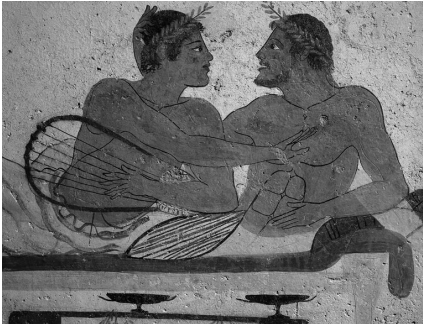
\includegraphics[scale = 0.4]{../images/TheLovers.PNG}
    \caption{The Lovers; detail of a fresco from the Tomb of the Diver (c. 480-470 BCE)}
    \label{fig:love}
\end{figure}

This has appeared in many scholarly works of homosexuality in the ancient world. However, based on our understanding of the ancient Greek past, this depiction is neither a representation of homosexuality nor of gayness unless we are to speak in an anachronistic (belonging to a period other than that portrayed), essentialist (objects have an underlying reality or true nature that one cannot observe directly) view.

\begin{qst}
    Should we then use the broader, more flexible category of queer, which denotes a site of marginalization from and resistance to dominant culture, to try to link the male-male eroticism of the past to the homosexuality of the present?
\end{qst}

If the paintings were modern they would fit into the context of ``queer." Indeed, the ultimate setting for the \textbf{er$\overline{\text{o}}$menos} and \textbf{erast$\overline{\text{e}}$s} in the painting is a homoerotic, homosocial afterlife.

\begin{rmk}
    In the context of their time, the paintings invite us to a space that was a privileged location of the Greek patriarchy---the symposium.
\end{rmk}

Indeed, the Tomb of the Diver paintings are like the pederastic (depicting intimacy between a male and young boy, usually in his teens) symposium scenes found on Attic pottery (pottery from the \textbf{Attica}, a historical region encompassing Athens) and described in philosophical and other Greek treatises. 

\begin{nte}
    The author argues that Ancient Greek societies were \textbf{homonormative} in that they privileged males and prioritized relationships between men through the institution of pederasty.
\end{nte}

The paintings show local Italic influences, especially of death sexuality, and banqueting that seem to have been borrowed from the Etruscans (civilization which controlled a majority of the Italian peninsula). However, in Etruscan depictions the male-female couple is privileged, but in the Tomb of the Diver it is the male-male couple that stands out. This suggests the Greeks of Poseidonia borrowed heavily from Etruscan conceptions of the afterlife, but adapted these ideas to suit their own solial milieu.

\begin{rmk}
    The eroticism and eschatology of the iconography of the Tomb of the Diver suggests the deceased was an initiate of the \textbf{Orphic cult}.
\end{rmk}

The Orphic cult followed a collection of beliefs and practices related to the mythical poet \textbf{Orpheus}. Previous scholarship ignored or subordinated the eroticism of the paintings to other concerns. The main exception to this is the analysis of \textbf{Cerchiai (1987)}, who instead subordinates the eschatological themes to the erotic. The author attempts to provide a more balanced approach.

\begin{nte}
    The author argues that the Orphic rites were, in much more of a Greek than an Etruscan fashion, both homosocial and homoerotic. In Orphic though, the symposium served both as a means to worship Dionysus and other gods in this life, and as an image of the eternal hereafter in the next life.
\end{nte}




\subsection{The Paintings}


The paintings in the Tomb have been dated to approximately \textbf{480-470 BCE} based on pottery in the tomb. The two long sided slabs depict partygoers lounging on couches at what has been identified as a symposium.

\begin{figure}[H]
    \centering
    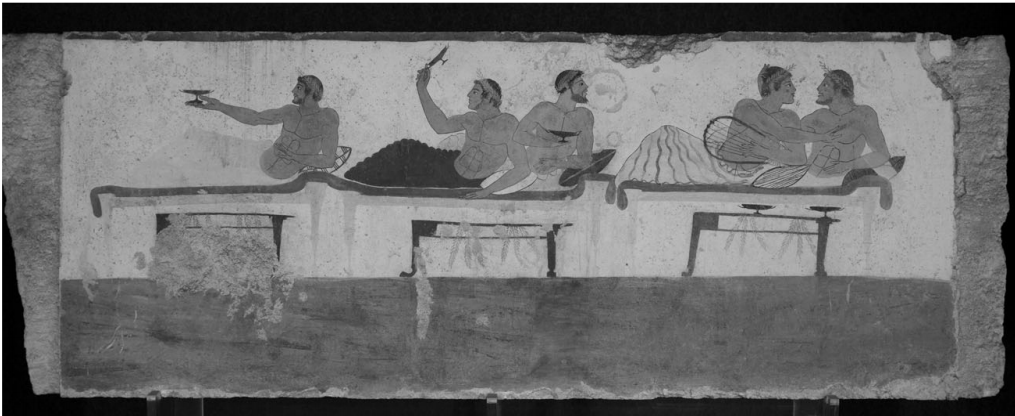
\includegraphics[scale = 0.3]{../images/North.PNG}
    \caption{North wall of Tomb of the Diver}
    \label{fig:north}
\end{figure}

\begin{figure}[H]
    \centering
    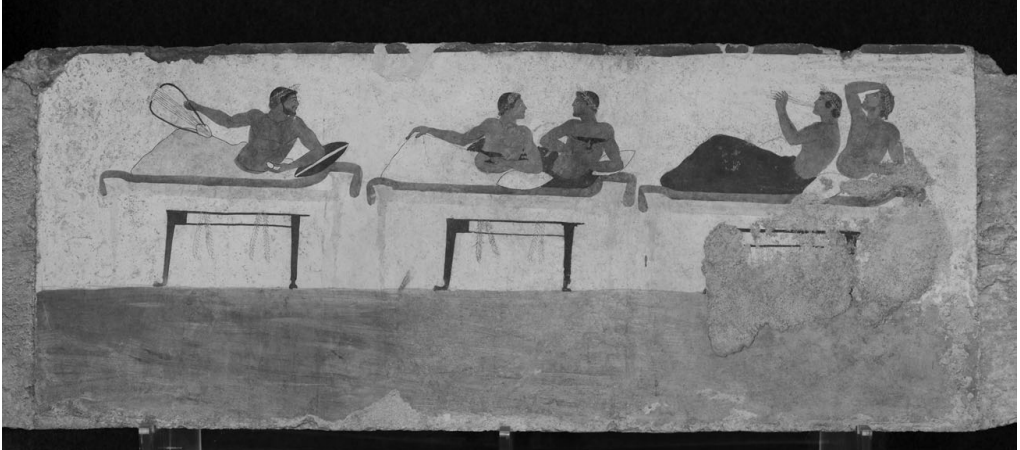
\includegraphics[scale = 0.3]{../images/South.PNG}
    \caption{South wall of Tomb of the Diver}
    \label{fig:south}
\end{figure}

Most of the male guests appear in couples, and the celebrated pair in Figure \ref{fig:love} have been labeled \textbf{gli amanti ``the lovers"} by Mario Napoli, the archeologist who discovered the tomb. On the opposite wall one of the symposiasts is playing music while his couchmate holds his hand to his forehead, a gesture which has been interpreted to indicate a state of ecstasy. The symposiast on the left in Figure \ref{fig:south} is holding an egg, which has been identified as a symbol of the Greek Orphic religious movement (it symbolizes the belief in eventual reunification with a divine source---Phanes, also called Eros, the creator of all things, was an androgynous being who was originally thought to have hatched from a shell). On the middle couch (\textbf{klin$\overline{\text{e}}$}) of Figure \ref{fig:north} the symposiast has raised his \textbf{kylix} (wine drinking cup) at an angle indicating that he is playing \textbf{kottabos} (similar to modern-day darts). The dregs offered in kottabos in a symposium were done so in the name of an \textbf{er$\overline{\text{o}}$menos}.

\begin{figure}[H]
    \centering
    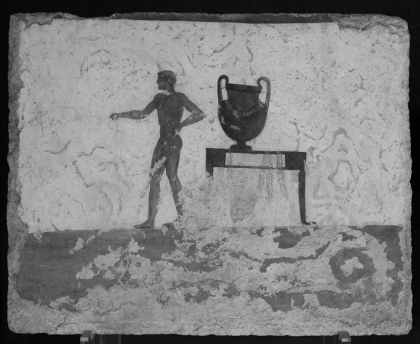
\includegraphics[scale = 0.3]{../images/East.PNG}
    \caption{East wall of Tomb of the Diver. Depicts a youth walking from a garlanded krater which appears to contain wine. The youth is most likely the designated wine pourer for the guests.}
    \label{fig:east}
\end{figure}


\begin{figure}[H]
    \centering
    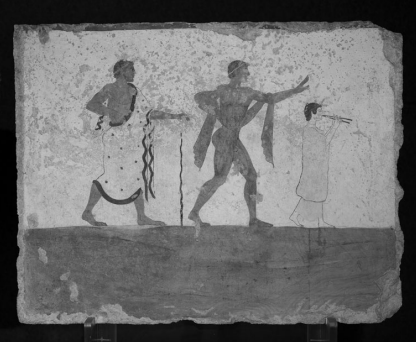
\includegraphics[scale = 0.3]{../images/West.PNG}
    \caption{West wall of Tomb of the Diver. A procession of symposiasts led by a female flautist followed by a naked youth with a blue scarf draped over his arms and a clothed bearded man.}
    \label{fig:west}
\end{figure}



\begin{figure}[H]
    \centering
    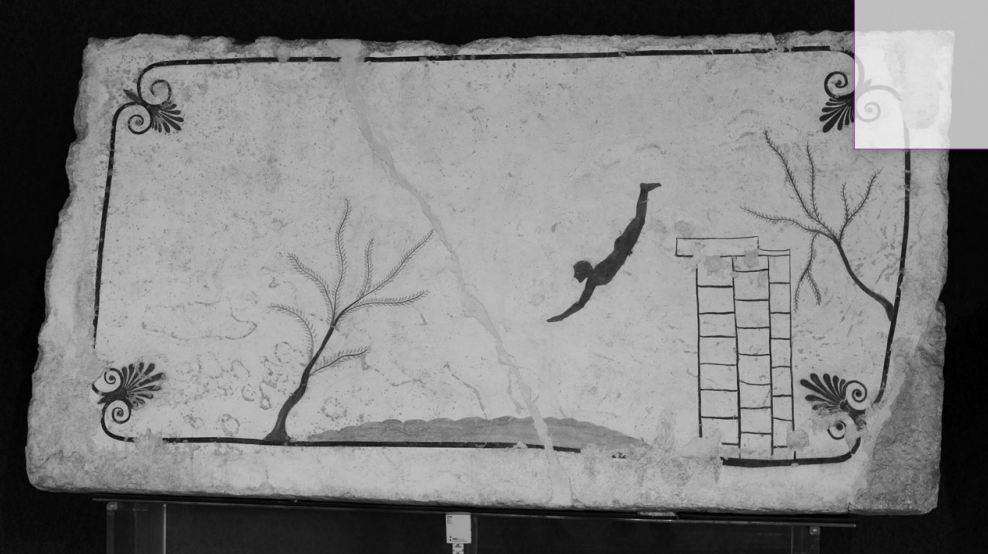
\includegraphics[scale = 0.3]{../images/Cover.PNG}
    \caption{Slab cover of Tomb of the Diver. A naked young man is pictured diving into a body of water.}
    \label{fig:slab}
\end{figure}


The Poseidonian paintings in the Tomb of the Diver, despite similarities in the symposium scenes, otherwise fall outside the norms of \textbf{Attic art}. The association of the symposium with the afterlife and of eschatology with eroticism are reflective of Etruscan influence, as \textbf{Pontrandolfo (1996)} has argued:

\begin{quotation}
    While full of Greek conceptual models, the paintings in the Diver's Tomb are in fact an exception, even as far as their contents are concerned, because they do not mirror the typical mental attitude of Greeks who would normally never decorate the interior of tombs with paintings, nor place the world of death together with that of the symposium, for the two worlds contradict each other. The homosociality of the symposium participants, nevertheless, is very Greek.
\end{quotation}

As with other Attic symposium scenes, the only female in the frescoes is a young flute girl. In contrast, Etruscan paintings show women, probably wives, at symposia.

\begin{figure}[H]
    \centering
    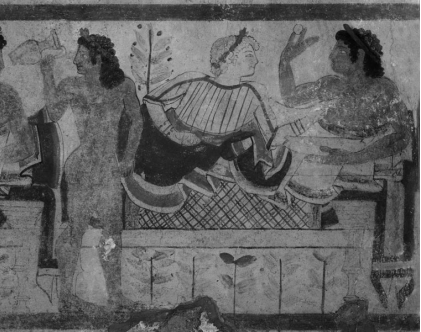
\includegraphics[scale = 0.3]{../images/Leopards.PNG}
    \caption{Tomb of the Leopards}
    \label{fig:leo}
\end{figure}

\begin{rmk}
    No other comparable funerary paintings from the fifth century have been discovered in the vicinity of Poseidonia.
\end{rmk}

Other painted tombs from the fourth century BCE have been found, but they date to the period after the Lucanian invasion/conquest of Poseidonia (when the name of the city was changed to Paestum), thus after the period of Greek rule of the \textbf{polis} of Poseidonia. Nonetheless, fourth-century male burials are usually accompanied by \textbf{kraters} and other wine vessels which suggest that, for men, the afterlife might include a symposium.

\subsection{Eschatology of the tomb's iconography}

Note that \textbf{eschatology} is the part of theology concerned with death, judgement, and the final destiny of the soul and humankind. 

\textbf{Napoli} interpreted the dive scene as \textbf{Pythagorean}, representing the purifying passage of the soul through water. But this fails to account for the relationship of the diver to the symposium scene. 

\textbf{Bianchi-Bandinelli (1970)} has asserted that the symposium scenes represent the heroic afterlife in the Isles of the Blessed beyond the western limits of the Mediterranean described by \textbf{Hesiod}, that the structure from which the diver leaps representes the \textbf{Pillar of Heracles}, and that the body of water he plunges into is the Atlantic Ocean, which represented the limits of the known world to the Greeks. However several centuries separate the time of Hesiod and the tomb, and the body of water into which the diver plunges looks much more like a small lake or spring than an ocean.

Note the diver, the association of the symposium with the afterlife, and the procession of the deceased are all themes that surface in Etruscan funerary art. The Greek colony of Poseidonia lay just to the south of Naples, and the polis shared a border along the River Sele, with ancient Campania. Campania was already ``deeply Etruscanized" by the end of the seventh century BCE, when Poseidonia was founded. The inhabitants of Poseidonia mingled and possibly intermarried with Etruscans and other native inhabitants of the region, so the influx of Etruscan eschatology into the region is not surprising. Inscriptions on an \textbf{olp$\overline{\text{e}}$} manufactured at Poseidonia and found at Fratte di Salerno contains short erotic verses involving persons with Greek, Etruscan, and other Italic names.

Although the association of the symposium with the afterlife is at first an Italic/Etruscan feature, the paintings do represent the attitude of at least some Greeks---those Greeks called ``Orphics" who followed the teachings of \textbf{Musaeus}. Indeed, Plato described the Orphic conception of the afterlife as a banquet where the reward is eternal drunkenness (attributed to Musaeus, who was either a son or friend to Orpheus).

\begin{nte}
    Orpheus was a prophet of Dionysus, and hence the ``Orphic" cult was associated with and perhaps even synonymous with the Dionysiac/Bacchic mysteries in ancient Southern Italy.
\end{nte}

Orphic beliefs demonstrate a number of commonalities with Etruscan eschatology, including:

\begin{enumerate}
    \item[(1)] a procession of the dead to a blessed afterlife;
    \item[(2)] a need to either pass through or drink water to reach that afterlife;
    \item[(3)] the representation of that afterlife as a banquet or symposium.
\end{enumerate}

By the fourth century BCE Plato refers to the ``Orphic" idea of the afterlie as a symposium being a reward for the just, whereas the unjust went to the house of Hades as punishment for their wrongdoings. This suggests that the Etruscan idea of the afterlife was borrowed by Greeks who adapted it for their own needs in the Orphic cult.

\begin{rmk}
    This is a radical departure from archaic Greek religion where humans went to the gloomy ``land of the shadows" described by Homer, save for a select few of the heroic race you transcended mortality to dwell in the paradise of the Elysian fields at the end of the earth described by Hesiod. On the other hand in Orphic belief the afterlife was a reunion with the gods, in the form of a symposium.
\end{rmk}

Some other Orphic initiates in nearby Greek colonies were buried with a tablet, considered by archeologists to be a type of passport which would give the Orphic initiate access to the afterlife. A fifth-century tablet found in Hipponium in Souther Italy contained a small text:

\begin{quotation}
    This (dictate) is sacred to Memory (for the \textbf{mystes} [initiate]) on the point of death. You will go to the well-built house of Hades, where, on the right, there lies a spring, and next to that a white cypress tree stands. There the souls of the dead seek refreshment. Do not even approach this spring. Beyond it you will find the cold water that runs from the lake of Memory, with its keeper to the fore, and they will ask you, with clear penetration, what you seek in the shades of murky Hades. Reply: ``I am the son of the Earth and of starry Heaven; I burn with thirst and I am fainting; quick, give me to drink the cold water that comes from the lake of Memory. They are merciful, as the king of the underworld wills, and will give you to drink from the lake of Memory; and when you have drunk you will travel the sacred path where the other \textbf{mystai} and \textbf{bakkhoi} proceed in glory."
\end{quotation}

In this context the procession depicted on the west wall of the tomb may be none other than a sacred procession of \textbf{bakkhoi} as mentioned in the tablet above.

However, some skepticism over the ``Orphic" associations in this text have been expressed because the deceased buried with it was a woman. What we can loosely term ``Orphic/Dionysiac" cults were marked by sex-segregated rites.

The elements of water and earth are also invoked in what \textbf{Clement of Alexandria} alleges is the writing of Orpheus himself:

\begin{quotation}
    Water is death for souls, But from water comes earth, from earth again water, and thence soul, rushing to all the ether.
\end{quotation}

Both Orpheus and Dionysus journey to the underworld and return from it in Greek myth, and it stands to reason that both of these mythical characters, the god and his prophet, were believed to have the power to intercede on behalf of the dead with the rulers of the underworld.

\subsection{The symposium and Orphic rites: Higher forms of knowledge, homosociality, and homoeroticism}

Orphic/Dionysiac mystery rites ultimately sought to provide the initatie with a better afterlife through the purification provided by traveling Orphic priests, or \textbf{orpheotelestai}. From a tablet in the Black Sea colony of Olbia dating to the fifth century BCE, one finds the text ``life death life truth," which seems to argue for reincanation at least once before reaching the Orphic afterlife of ``truth." ``Liberation from the wheel of life" in Orphism could be achieved, it was thought, through religious rites.

Beginning in the 480s BCE, and hence relevant to the Tomb of the Diver paintings, Attic vases show Orpheus surrounded by males only. \textbf{Phanocles} explains that Orpheus introduced ``male love" (\textbf{er$\overline{\text{o}}$tas arrenas}) to the Thracians. Eventually the Thracian women killed Orpheus out of jealousy for taking their husbands away from them. In terms of the pederasty and homosociality, the ``Orphic rite" has much in common with the Greek concept of the symposium.

According to \textbf{Cerchiai} the reveler would obtain access to higher forms of knowledge through the symposium. In the symposium, ``the phrase `wine and truth' was proverbial for those who talked frankly while inebriated."

\begin{nte}
    Sympotic discussions strove both to enlighten one's contemporaries with regard to politics but even more to educate the \textbf{er$\overline{\text{o}}$menoi} present, just as the Orphic rite strove to educate the initiate as to how to find an eternity of sympotic pleasure.
\end{nte}

The sexuality displayed is consistent with a neschatological Orphic reading. \textbf{Cerchiai} suggests that the procession on the west wall of the tomb is an erotic hunt, in which the older bearded man is chasing the younger, nude man.


\subsection{Ancient Paintings, Modern Queerness}

The sympotic scenes denote what is, for all intents and purposes, a specifically ancient context. The symposium scene was more than a drinking party; it was a ritual, wherein a libation was poured to the god Dionysus, paeans were sung, and divination was sought through the game of kottabos. The Tomb of the Diver symposium seems to represent both the best of this life and hereafter, given Plato's description of the Orphic afterlife as sympotic. 

\begin{rmk}
    In the social development of a Greek citizen, the youth was meant to begin his sexual and social development as an \textbf{er$\overline{\text{o}}$menos}, then, when his beard came in, to become the \textbf{erast$\overline{\text{e}}$s}, and finally, around the age of $30$, to give up youthful same-sex \textbf{er$\overline{\text{o}}$s} and marry.
\end{rmk}

This was normative. Understanding ``queerness" as being identified with marginalization and transgression, the author argues that there is nothing ``queer" going on, but instead the paintings should be called ``homonormative," in the ancient Greek context, defining the centrality of social and/or erotic relationships among men to the institutions such as the symposium, that reify and promote exclusive male privilege in the power structures of society.

According to \textbf{Cohen (1991)}:
\begin{quotation}
    when an Athenian man courts a boy he does so according to the normative expectations ofthe boy, his family, and the community of which he is a part (all social interaction is normatively structured by such expectations, though these expectations may conflict or reflect moral ambivalences about the conduct). Yet the norms reflected in such expectations do not simply determine his behavior. He possesses the knowledgeability that almost all individuals have about the norms, values, beliefs, and practical expectations of the society in which they live. This knowledgeability enables individuals to influence evaluations of their behavior by interpreting and manipulating their words and deeds and the normative categories by which they are judged.
\end{quotation}

While little is known of the customs and social history of ancient Poseidonia, its mother city of \textbf{Sybaris}, itself an \textbf{Achaean colony} that was known for its wealth and luxurious way of life in antiquity had a few more details. The inhabitants of Sybaris were the most indulgent of the Western Greeks. The Sybarites were known to like and have befriended the Etruscans to the north and the Ionians to the east. 

\begin{qst}
    Could this indicate Etruscan influence on Poseidonian sexuality? 
\end{qst}

Note the Poseidonians lived between the Sybarites and the Etruscans, and had absorbed some of the Etruscan ideology of the afterlife into their own eschatology. Inscriptions on an \textbf{olp$\overline{\text{e}}$} made in Poseidonia nad found in a tomb at nearby Fratte di Salerno suggests that same-sex activity was enjoyed between Greeks and Etruscans:

\begin{quotation}
    Apollodorus loves Kscylla 

    Wolchas buggers Apollodorus

    Onatas loves Nikso

    Hybrichus has love Parmynio.
\end{quotation}

Five males (Apollodorus, Wolchas, Onatas, Hubrichus, and Parmynio) and two females (Ksylla and Nikso) are named. Athenaeus points out that the Etruscan men enjoyed sex with both boys (\textbf{paides}) and young men (\textbf{meirakia}), a term that refers approximately to twenty-yera-old males.

\subsection{Conclusion}

The paintings analyzed suggest that the idea of a drunken, sexy hereafter derived from an Etruscan context was imported into Greek thought and altered to fit Greek norms of homosociality and pederasty in the ``Orphic" religious movement. The Tomb of the Diver paintings display a relationship between male-male eroticism and the afterlife that is Orphic.

The Tomb of the Diver paintings show a pederastic ideal, even if it is not as stringent as the Athenian model. The close proximity of Poseidonia to Etruscan and othe Italic communities may offer a rationale for this phenomenon.





\section{Notes on Analysis and Societal Context}
\label{sec:SocCont3}

\begin{rmk}
    The author begins by describing the five paintings before preceeding to a survey of the secondary scholarship on the paintings, and then presenting their own interpretations. Finally, they return to the question of the use of images to mark homosexuality or gay identity, and argue that the scene in the painting is neither gay nor queer, but rather offers a ``homonormative" paradigm.
\end{rmk}

\begin{nte}
    As the author notes, to be useful for analysis of ancient Greek evidence queer theory must be adapted and refined as concepts like ``heteronormative" do not really apply.
\end{nte}



%
% \begin{acknowledgement}
% If you want to include acknowledgments of assistance and the like at the end of an individual chapter please use the \verb|acknowledgement| environment -- it will automatically render Springer's preferred layout.
% \end{acknowledgement}
%
% \section*{Appendix}
% \addcontentsline{toc}{section}{Appendix}
%


% Problems or Exercises should be sorted chapterwise
\section*{Problems}
\addcontentsline{toc}{section}{Problems}
%
% Use the following environment.
% Don't forget to label each problem;
% the label is needed for the solutions' environment
\begin{prob}
\label{prob1}
A given problem or Excercise is described here. The
problem is described here. The problem is described here.
\end{prob}

% \begin{prob}
% \label{prob2}
% \textbf{Problem Heading}\\
% (a) The first part of the problem is described here.\\
% (b) The second part of the problem is described here.
% \end{prob}

%%%%%%%%%%%%%%%%%%%%%%%% referenc.tex %%%%%%%%%%%%%%%%%%%%%%%%%%%%%%
% sample references
% %
% Use this file as a template for your own input.
%
%%%%%%%%%%%%%%%%%%%%%%%% Springer-Verlag %%%%%%%%%%%%%%%%%%%%%%%%%%
%
% BibTeX users please use
% \bibliographystyle{}
% \bibliography{}
%


% \begin{thebibliography}{99.}%
% and use \bibitem to create references.
%
% Use the following syntax and markup for your references if 
% the subject of your book is from the field 
% "Mathematics, Physics, Statistics, Computer Science"
%
% Contribution 
% \bibitem{science-contrib} Broy, M.: Software engineering --- from auxiliary to key technologies. In: Broy, M., Dener, E. (eds.) Software Pioneers, pp. 10-13. Springer, Heidelberg (2002)
% %
% Online Document

% \end{thebibliography}


%%%%%%%%%%%%%%%%%%%%% chapter.tex %%%%%%%%%%%%%%%%%%%%%%%%%%%%%%%%%
%
% sample chapter
%
% Use this file as a template for your own input.
%
%%%%%%%%%%%%%%%%%%%%%%%% Springer-Verlag %%%%%%%%%%%%%%%%%%%%%%%%%%
%\motto{Use the template \emph{chapter.tex} to style the various elements of your chapter content.}
\chapter{Gravity as Geometry}
\label{GravGeomBitch} % Always give a unique label
% use \chaptermark{}
% to alter or adjust the chapter heading in the running head



\abstract{To be completed once done}

\section{The Equivalence Principle}
\label{sec:equivPrinc}

The equivalence principle is regarded as a heuristic idea whose central content is incorporated automatically and precisely in general relativity where appropriate. The equality of gravitational and inertial mass is essential for this argument. Einstein's equivalence principle is the idea that there is no experiment that can distinguish a uniform acceleration from a uniform gravitational field. This implies that light falls in a gravitational field.


\section{Clocks in a Gravitational Field}
\label{sec:clockGrav}

When the gravitational field is nonuniform the equivalence principle holds only for experiments in laboratories that are small enough and that take place over a short enough period of time that no nonuniformities in $\Phi$ can be detected.

\begin{rmk}
    The \textbf{Equivalence Principle} states that experiments in a sufficiently small freely falling laboratory, over a sufficiently short time, give results that are indistinguishable from those of the same experiments in an intertial frame in empty space.
\end{rmk}


\section{The Global Positioning System}
\label{sec:GlobPos}

\section{Spacetime is Curved}
\label{sec:spaceCurve}

\begin{qst}
    What is the explanation of the difference between the rates at which signals are emitted and received at two different gravitational potentials?
\end{qst}

One explanation is that gravity affects the rates at which clocks run. In the absence of any gravitational field, two clocks at rest in an inertial frame of flat spacetime both keep track of the time of that frame. In the presence of a gravitational field, the spacetime remains flat, but clocks run at a rate that is a factor $(1+\Phi/c^2)$ different from their rates in empty spacetime, where $\Phi$ is the gravitational potential at the location of the clock. Clocks run faster where $\Phi$ is positive and slower where $\Phi$ is negative.


However, it is simpler, more economical, and ultimately more powerful to recognize that clocks correctly measure timelike distances in spacetime and that its geometry is curved.

\section{Newtonian Gravity in Spacetime Terms}
\label{sec:NewtGrav}

We consider a simple model that will introduce a clight curvature that will explain geometrically the behaviour of clocks we have been discussing. We specify the \textbf{Static Weak Field Metric} by \begin{equation}
    \boxed{ds^2 = -\left(1+\frac{2\Phi(x^i)}{c^2}\right)(cdt)^2+\left(1-\frac{2\Phi(x^i)}{c^2}\right)(dx^2+dy^2+dz^2)}
\end{equation}

where the gravitational potential $\Phi(x^i)$ is a function of position satisfying the Newtonian field equation and assumed to vanish at infinity. For example, outside Earth $\Phi(r) = -GM_{\oplus}/r$. 

\subsection{Rates of Emission and Reception}


Consider signals propagating along the $x$-axis emitted at one location, $x_A$, and received at another, $x_B$. The world line of a light signal won't be a $45^{\circ}$ straight line, as in flat spacetime. But the world lines of both signals will have the same shape because the geometry is independent of $t$. The signals are therefore received at $B$ with the same coordinate separation $\Delta t$ as they were emitted with at $A$. But a coordinate separation $\Delta t$ corresponds to two different proper time intervals at the two locations. The coordinate separations between the two emissions at location $x_A$ are $\Delta t$ and $\Delta x = \Delta y = \Delta z = 0$. The proper time separation $\Delta \tau_A$ between these events is $d\tau^2 = -ds^2/c^2$ so $$\Delta \tau_A = \left(1+\frac{\Phi_A}{c^2}\right)\Delta t$$
accurate to order $1/c^2$, where $\Phi_A = \Phi(x_A,0,0)$. Similarly, on reception $$\Delta \tau_B = \left(1+\frac{\Phi_B}{c^2}\right)\Delta t$$
Eliminating $\Delta t$ between these two relations gives $$\Delta \tau_B = \left(1+\frac{\Phi_B-\Phi_A}{c^2}\right)\Delta \tau_A$$


\subsection{Newtonian Motion in Spacetime Terms}

The principle that a free particle follows a path of extremal proper time between ny two points also gives the motion of a particle in a gravitational potential $\Phi$ in the spacetime geometry described previously. The proper time between two points $A$ and $B$ in spacetime depends on the world line between them and is given by $$\tau_{AB} = \int_A^B\left[\left(1+\frac{2\Phi}{c^2}\right)dt^2-\frac{1}{c^2}\left(1-\frac{2\Phi}{c^2}\right)(dx^2+dy^2+dz^2)\right]^{1/2}$$
integrated along the world line connecting $A$ and $B$. All of our considerations have been accurate only to first order in $1/c^2$, and to that order this becomes under a $t$ parameterization $$\tau_{AB} \approx \int_A^Bdt\left[1-\frac{1}{c^2}\left(\frac{1}{2}\left|\left|\vec{v}\right|\right|^2-\Phi\right)\right]$$
The world line that extremizes the proper time between $A$ and $B$ will extremize the combination $$\int_A^Bdt\left(\frac{1}{2}\left|\left|\vec{v}\right|\right|^2-\Phi\right)$$
since the first term in the original integral doesn't depend on which world line is traveled. The conditions for an extremum are Lagrange's equations, following from the Lagrangian $$L\left(\frac{d\vec{x}}{dt},\vec{x}\right) = \frac{1}{2}\left(\frac{d\vec{x}}{dt}\right)^2-\Phi(\vec{x},t)$$
If multiplied by the mass, this is just the Lagrangian for a nonrelativistic particle moving in the gravitational potential $\Phi$. Lagrange's equations imply $$\frac{d^2\vec{x}}{dt^2} = -\nabla\Phi$$
which, when both sides are multiplied by $m$ is just $\vec{F} = m\vec{a}$.

\begin{table}[H]
    \centering
    \caption{Newtonian and Geometric Formulations of Gravity Compared}
    \begin{tabular}{p{4cm}p{5cm}p{5cm}p{4cm}}
        \hline
        & Newtonian & Geometric Newtonian & General Relativity \\ \hline
        What a mass does & Produces a field $\Phi$ causing a force on other masses $-m\nabla \Phi$ & Curves spacetime $ds^2 = -\left(1+\frac{2\Phi}{c^2}\right)(cdt)^2 + \left(1-\frac{2\Phi}{c^2}\right)(dx^2+dy^2+dz^2)$ & Curves spacetime \\
        Motion of a particle & $m\vec{a} = \vec{F}$ & Curve of extremal proper time (first order in $1/c^2$) & Curve of extremal proper time \\ 
        Field equation & $\nabla^2\Phi = +4\pi G\mu$ & $\nabla^2\Phi = +4\pi G\mu$ & Einstein's equation \\ \hline 
    \end{tabular}
    \label{tab:newtGeom}
\end{table}

The Newtonian gravitational law is inconsistent with the principles of special relativity because it specifies an instantaneous interaction between bodies. The asymmetry between space and time in the metric shows this in anothe rway. Even in a geometric formulation Newtonian gravity is inconsistent with special relativity. A fully relativisticm geometric theory of gravity would treat space and time on a symmetric footing.








% \begin{acknowledgement}
% If you want to include acknowledgments of assistance and the like at the end of an individual chapter please use the \verb|acknowledgement| environment -- it will automatically render Springer's preferred layout.
% \end{acknowledgement}
%
\section*{Appendix}
\addcontentsline{toc}{section}{Appendix}




% Problems or Exercises should be sorted chapterwise
\section*{Problems}
\addcontentsline{toc}{section}{Problems}
%
% Use the following environment.
% Don't forget to label each problem;
% the label is needed for the solutions' environment
\begin{prob}
\label{prob1}
A given problem or Excercise is described here. The
problem is described here. The problem is described here.
\end{prob}

% \begin{prob}
% \label{prob2}
% \textbf{Problem Heading}\\
% (a) The first part of the problem is described here.\\
% (b) The second part of the problem is described here.
% \end{prob}

%%%%%%%%%%%%%%%%%%%%%%%% referenc.tex %%%%%%%%%%%%%%%%%%%%%%%%%%%%%%
% sample references
% %
% Use this file as a template for your own input.
%
%%%%%%%%%%%%%%%%%%%%%%%% Springer-Verlag %%%%%%%%%%%%%%%%%%%%%%%%%%
%
% BibTeX users please use
% \bibliographystyle{}
% \bibliography{}
%


% \begin{thebibliography}{99.}%
% and use \bibitem to create references.
%
% Use the following syntax and markup for your references if 
% the subject of your book is from the field 
% "Mathematics, Physics, Statistics, Computer Science"
%
% Contribution 
% \bibitem{science-contrib} Broy, M.: Software engineering --- from auxiliary to key technologies. In: Broy, M., Dener, E. (eds.) Software Pioneers, pp. 10-13. Springer, Heidelberg (2002)
% %
% Online Document

% \end{thebibliography}


%%%%%%%%%%%%%%%%%%%%% chapter.tex %%%%%%%%%%%%%%%%%%%%%%%%%%%%%%%%%
%
% sample chapter
%
% Use this file as a template for your own input.
%
%%%%%%%%%%%%%%%%%%%%%%%% Springer-Verlag %%%%%%%%%%%%%%%%%%%%%%%%%%
%\motto{Use the template \emph{chapter.tex} to style the various elements of your chapter content.}
\chapter{Description of Curved Spacetime}
\label{CurvSpac} % Always give a unique label
% use \chaptermark{}
% to alter or adjust the chapter heading in the running head



\abstract{To be completed once done}

\section{Coordinates}
\label{sec:Coord}


A line element specifies a geometry, but many different line elements describe the same spacetime geometry because different coordinate systems can be used. A good coordinate system provides unique labels for each point in spacetime. However, most coordinate systems only do this locally. Even polar coordinates fails to uniquely label points on the $\theta = 0$ axis. The singularities in most coordinate systems mean that different overlapping coordinate patches must be used to cover spacetime so that every point is labeled by a nonsingular set of coordinates.


\section{Metric}
\label{sec:metRic}

To describe a general geometry we use a system of four coordinates, $x^{\alpha}$, to label the points and specify the line element giving the distance, $ds^2$, between nearby points separated by coordinate intervals $dx^{\alpha}$. That line element will have the form \begin{equation*}
    \boxed{ds^2 = g_{\alpha\beta}(x)dx^{\alpha}dx^{\beta}}
\end{equation*}
where $g_{\alpha\beta}(x)$ is a symmetric, position-dependent matrix called the \textbf{metric}.


\section{The Summation Convention}
\label{sec:summConv}

\begin{enumerate}
    \item The location of the indices must be respected: superscripts for coordinates and vector components and subscripts for the metric.
    \item Repeated indices always occur in superscript-subscript pairs and imply summation.
    \item Indices that are not summed are called free indices.
\end{enumerate}



\section{Light Cones and World Lines}
\label{sec:LightWorld}

Points separated from $P$ by infinitesimal coordinate intervals $dx^{\alpha}$ can be timelike separated, spacelike separated, or null separated as the square of their distance away defined by the metric satisfies \begin{align*}
    ds^2 &< 0 \tag{timelike separation} \\
    ds^2 &= 0 \tag{null separation} \\
    ds^2 &> 0 \tag{spacelike separation}
\end{align*}
Light rays move along null curves in spacetime along which $ds^2= 0$.

Particles move on timelike world lines which can be specified parametrically by four functions $x^{\alpha}(\tau)$ of the distance $\tau$ along them.
\begin{defn}
    The distance between a point $A$ and a point $B$ along a timelike worl line is given by \begin{equation*}
        \tau_{AB} = \int_A^B[-g_{\alpha\beta}(x)dx^{\alpha}dx^{\beta}]^{1/2}
    \end{equation*}
    where the integral is along the world line.
\end{defn}

The global arrangement of light cones is called the spacetime's \textbf{causal structure}.


\section{Length, Area, Volume, and Four-Volume for Diagonal Metrics}
\label{sec:measurements}

In this section suppose $ds^2 = g_{\alpha\alpha}dx^{\alpha}dx^{\alpha}$ is a diagonal metric. The proper lengths of a segment will be of the form $d\ell^{1} = \sqrt{g_{11}}dx^{1}$. Since the coordinates are orthogonal, the area element created by the region spanned by two line segments is $$dA = d\ell^2d\ell^3 = \sqrt{g_{11}g_{22}}dx^1dx^2$$
For three-volume $$dV = \sqrt{g_{11}g_{22}g_{33}}dx^1dx^2dx^3$$
For a metric of signature $(1,3)$, the four-volume is $$dv = \sqrt{-\det(g_{\alpha\beta})}d^4x$$







% \begin{acknowledgement}
% If you want to include acknowledgments of assistance and the like at the end of an individual chapter please use the \verb|acknowledgement| environment -- it will automatically render Springer's preferred layout.
% \end{acknowledgement}
%
\section*{Appendix}
\addcontentsline{toc}{section}{Appendix}




% Problems or Exercises should be sorted chapterwise
\section*{Problems}
\addcontentsline{toc}{section}{Problems}
%
% Use the following environment.
% Don't forget to label each problem;
% the label is needed for the solutions' environment
\begin{prob}
\label{prob1}
A given problem or Excercise is described here. The
problem is described here. The problem is described here.
\end{prob}

% \begin{prob}
% \label{prob2}
% \textbf{Problem Heading}\\
% (a) The first part of the problem is described here.\\
% (b) The second part of the problem is described here.
% \end{prob}

%%%%%%%%%%%%%%%%%%%%%%%% referenc.tex %%%%%%%%%%%%%%%%%%%%%%%%%%%%%%
% sample references
% %
% Use this file as a template for your own input.
%
%%%%%%%%%%%%%%%%%%%%%%%% Springer-Verlag %%%%%%%%%%%%%%%%%%%%%%%%%%
%
% BibTeX users please use
% \bibliographystyle{}
% \bibliography{}
%


% \begin{thebibliography}{99.}%
% and use \bibitem to create references.
%
% Use the following syntax and markup for your references if 
% the subject of your book is from the field 
% "Mathematics, Physics, Statistics, Computer Science"
%
% Contribution 
% \bibitem{science-contrib} Broy, M.: Software engineering --- from auxiliary to key technologies. In: Broy, M., Dener, E. (eds.) Software Pioneers, pp. 10-13. Springer, Heidelberg (2002)
% %
% Online Document

% \end{thebibliography}


%%%%%%%%%%%%%%%%%%%%% chapter.tex %%%%%%%%%%%%%%%%%%%%%%%%%%%%%%%%%
%
% sample chapter
%
% Use this file as a template for your own input.
%
%%%%%%%%%%%%%%%%%%%%%%$% Springer-Verlag %%%%%%%%%%%%%%%%%%%%%%%%%%
%\motto{Use the template \emph{chapter.tex} to style the various elements of your chapter content.}
\chapter{Fertility control in ancient Rome}
\label{FertContInRome} % Always give a unique label
% use \chaptermark{}
% to alter or adjust the chapter heading in the running head


%%% Questions to think about
%The \textbf{Thesis} or general sense of the article is ...

%The \textbf{method} the author uses to argue their point is ...

%In their \textbf{analysis} the author uses tools such as ...
% How do they look at the evidence? Do they place it in some theoretical framework? (i.e. gender studies, music studies, etc.)

%Additionally they conclude ...
% How does this compare to others throughout time? What is the societal context?

%What connections does the author portray with regard to \textbf{space}, \textbf{relationships}, \textbf{occupation}, and \textbf{religion}.


\abstract{}

\section{Questions and Remarks}
\label{sec:QR6}


\begin{qst}
    How was Fertility percieved and understood in ancient Rome?
\end{qst}


\begin{qst}
    What methods did ancient Romans use to control women through fertility?
\end{qst}


\begin{qst}
    Were the methods deployed sufficiently effective to qualify as `control', and was it `fertility' that was being acted on through adoption and exposure?
\end{qst}




\section{First Reading}
\label{sec:FirRead6}


\begin{nte}
    One key shift in the history of human procreation is from societies in which the dominant fertility project was the production of helathy children to those in which the limitation of that production dominates.
\end{nte}

The reproduction of some groups is always enabled and encouraged more than others.

Agency in the fertility domain, particularly female agency, should not be restricted to action around contraception and abortion, but understood more holistically, as recent scholarship on medicine and childbearing in medieval Europe has emphasized.

\begin{rmk}
    Behaviour was not bound simply to the number of children already born, but also to their sex and survivorship, among other considerations.
\end{rmk}


The author notes the following quote with regard to the term `fertility control':

\begin{quotation}
    While helpful in linking the prevention and promotion of procreation, the term may be too modern for centuries before the twentieth. People have always aimed to achieve certain objectives for family continuity and population size, individual health and happiness, but their conceptual and practical tools have changed.
\end{quotation}


`Control' is a modern reproductive term. There is an issue about whether `control' sets the efficacy bar too high for the pre-modern world: whether, or to what extent, success in respect to or at least real purchase on the challenges and aims involved is required to use this language. There is also the sense in which `control' has now become an aim in itself rather than a means to an end, and so perhaps lacks the categorical stability necessary to do the requisite heuristic work.


\subsection{Fertility \textit{Control}}

Circa 100 CE in Rome, the noted physician \textbf{Soranus of Ephesus} composed his \textbf{Gynecology}, the only such dedicated treatise to survive from the early Roman Empire. Soranus traveled from his birthplace to the imperial capital via the medical schools of \textbf{Alexandria}, and continued to write in his native Greek. Greek was still the dominant language of learned medicine.

\begin{rmk}
    Soranus offered instructions about how to have healthy children to Roman elite, through opposition to and criticism of past medical authorities. He positioned himself against the traditional Hippocratic view that female health depended on generation, arguing instead that women's physical well-being was undermined by her `child-production' (\textbf{teknopoia}).
\end{rmk}

Soranus' pro-procreative program started with female anatomy and moved onto a systematic study of all the processes involved in generation, from menstruation to birth and the care of the newborn. Soranus insisted that girls pass the first occurrence of menstruation and become physically mature before marrying. This was somewhat at odds with elite practice in the Roman empire. Soranus argued that questions about the fertility of any prospective pride should accompany the customary inquiries.

\begin{nte}
    All evidence indicates that the Roman elite stuck to their traditional interests in birth, money, and looks, instead of heavily considering the fertility of their bride. The women's childbearing prowess was something to be proved. THe only women who posses the virtue of ``\textbf{fecunditas}", in the Annals of the Roman historian Tacitus, for instance, have already born children.
\end{nte}

Soranus' answer to conception followed the Hippocratic view that women are most likely to concieve as their periods are dwindling and stopping. For the rest, body and soul must be in the right condition, feeling good and appropriately inclined.

\begin{rmk}
    In modern medicine, the `fertile window' refers to the six days during which heterosexual intercourse can result in pregnancy, those being the five days before and the day of ovulation itself. So this does not align with Soranus' best time. However, both the menstrual and ovulatory cycles are somewhat variable.
\end{rmk}

Guidance of care for the pregnant woman had three stages: 
\begin{enumerate}
    \item guarding the deposited seed
    \item alleviating the ensuing symptoms, such as those associated with \textbf{kissa} (characterized by cravings, nausea, and general digestive disarray)
    \item Aim at perfecting the embryo and preparing for the demans of birth.
\end{enumerate}
Every aspect of a woman's life was to be regulated.



\begin{nte}
    The first book of the \textbf{Gynecology} ends with a chapter on contraception and abortion. Soranus believed that childbearing uses up resources, saps vigor, and causes premature aging. Thus Soranus opened up conceptual space in which talk of family limitation could occur, within the pro-procreative program.
\end{nte}

The items and actions which prevent conception were called \textbf{sullepsis} or `non-birthers' \textbf{atokia}, and those which `destroy what has been conceived' were called \textbf{phthoria}.

\begin{rmk}
    `Destruction of what is carried' was controversial at the time. The opposition called Hippocrates as a witness, who said `I will give no woman an abortive', and asserted that the medical art must guard and preserve what has been generated by nature.
\end{rmk}

The proponents of judgement were mainly motivated by preventing dangers in birth, and they said the same about contraceptives. Soranus concurred with this. 

Soranus' contraceptive presecriptions can be roughly divided into three:
\begin{enumerate}
    \item The first was that the `best time' for procreative sex should be avoided.
    \item The second involved applications to the mouth of the womb prior to intercourse, preventing the entry or retention of the seed.
    \item The last were oral contraceptives.
\end{enumerate}

For the thirty days after conception do the opposite of what Soranus advised to guard the deposited seed.

\begin{nte}
    Several of the ingredients listed by Soranus have been identified as having fertility suppressing effects in a range of ethnobotanical and laboratory studies.
\end{nte}

The work of John Riddle, who was the first to survey this evidennce in relation to ancient medical writings, has been subject to sustained criticism ever since: its orientation, presuppositions, methodology, and conclusions have all been called into question. For instance, discovering what modern species might be designated by ancient plant names is far from straightforward.

Soranus explicitly located his discussion of contraceptives and abortives within marriage. In pharmacological contexts or works on medical materials, actual engagement with the business of prevention or destruction occurred in association with prostitution. 

\begin{rmk}
    The philosophical poet Lucretius, writing his Latin epic \textbf{On the Nature of THings} in the last decades of the Roman Republic, had asserted that women themselves can `prevent or resist' conception, by pulling away and becoming limp as a man climaxes. This technique however belongs to `\textbf{scorta}' (`whores'), who wish to minimize their chances of becoming pregnant and maximize their client's pleasure.
\end{rmk}

The second book of the \textbf{Gynecology} covers the business of normal birth and the ensuing care of both mother and baby. There are two important points in the detailed descriptions and instructions:
\begin{enumerate}
    \item First is the section on how the midwife (\textbf{maia}) was to recognize whether the infant she had just delivered was fit for rearing or not. The main positive indicators were that the mother had enjoyed good health during pregnancy, birth had occurred at the proper time, the newborn had cried vigorously when placed on the ground, and was well-formed in all its parts. At the end of the day it was the father's decision to rear or expose (i.e. to put the new-born out to die or for someone else to raise).
    \item The other issue of interest is the nutrition of the newborn. Soranus favored wet-nursing, aligning himself with the dominant elite practice of the early Empire, and against arguments by some philosophers and traditional moralists that women should nurse their own infants.
\end{enumerate}

The later half of the \textbf{Gynecology} deals with the diseases of women, in which dangers and damaging impact of pregnancy and parturition loom large. Difficult birth is referred to as \textbf{dustokia}. The sections on several of these uterine ailments are not preserved in their original Greek, but, apart from their headings, survive only in the later `Latinizations' of the \textbf{Gynecology} of the fifth-centery CE North African physician Caelius Aureliunus and his less firmly located successor \textbf{Muscio}. Similarly, the contents of the final chapter in book three of Soranus' composition, listed as `On non-generation (\textbf{agonia}) and non-conception (\textbf{asullepsia})' are transmitted only in Latin. 

All of the failures associated with being `sterile', in latin `\textbf{Sterilitas}', occur in the female body according to Soranus, the cause may lie with either party. All of the reasons can be treated, mostly dietetically if addressing the overall somatic condition, and through pharmacological applications or surgery if the problem is more localized and specific.

There were non-medical courses of action available to those struggling to have children in the Roman Empire. Generative failure could be caused by some sort of incongruity or incompatibility between the couple having intercourse. The suggested remedy was changing partners for better results. The formulations were mostly vague, but Lucretius clearly recommended divorce and remarriage in contexts where no progeny had been forthcoming.


\begin{nte}
    By the time Lucretius wrote his didactic epic in the first centure BCE, divors and remarriage were legally (if not practically) straightforward for both parties at Rome, especially if there no no surviving offspring. This was a variation on a key theme in Roman matrimony---the main reason for divorce in the late Republic and early empire was to remarry, for political, economic, or generative purposes.
\end{nte}

Soranus had an apparent omission of the reltational aspects of infertility. A range of texts from the imperial period demonstrate that dream interpreters, astrologers and fortune-tellers were often consulted about the production of children, pregnancy, birth, and the prospects of the new-born. The point here is simply to return to the pro-procreative shape of Roman society, with which this section opened.

Note that although not all the resources for the generative project were accessible to those below the elite, many were, at lesat in some form. Maximum effectiveness still resides in infant exposure and adult adoption, however, so it is to these phenomena we now turn.

\subsection{\textit{Fertility} Control}

As \textbf{Soranus} assumed, in the Roman world birth was followed by a decision about whether to rear the newborn. A positive judgement meant being welcomed into the family and community, while a negative one entailed the separation of the child from their natal famly through exposure, their being put out (\textbf{ekthesis}) either to die or be picked up and raised by someone else. The main reason for third party rescue was to bring up the infant as a slave. \textbf{Exposure} was about separation or rejection, not about the fate of the child. It was a means of regulating family size and family composition.

\begin{rmk}
    Soranus described a physical assessment of suitability to rear, one that was entirely gender neutral, but other ancient sources and modern scholarship raise the possibility of selectivity by sex in these post-parturition judgements, a selectivity that favored boys over girlds.
\end{rmk}

Issues of sex and disability surely played a role in Roman decision making about raising children, but in complex and relative rather than absolute ways.

Control can be exercised over quantity and quality, and the efficacy of \textbf{expositio} is obvious in respect to both. Until the development of reliable fetal sex discernment tests in the twentieth century, exposure and infanticide were the only means of sex selection in relation to offspring. 

\begin{qst}
    Did the Roman sources themselves include \textbf{expositio} with other forms of family limitation or considered it as a distinct practice? Where did it fit in the overall demographic system of the Roman world?
\end{qst}

Soranus' approach was essentially inclusive, covering contraception, abortion, and exposure, as well as infertility treatments, in a single treatise. Soranus' role was limited by the role of the \textbf{maia} as reporter's of the newborn's physical condition to those in the family who would make the actual decision: most critically, the father, in whose power (\textbf{patria potestas}) any child raised would most likely be.

Roman law made all legitimate offspring, female and male, automatic heirs (\textbf{sui heredes}) who had to be left a fair share of the estate unless explicitly disinherited.

\begin{nte}
    A couple decades before Soranus was writing, the Stoic moralist \textbf{Musonius Rufus} argued strongly in support of the thesis that all children born should be raised, which was more or less the positon of the \textbf{Stoa}.
\end{nte}

Musonius mainly had an issue with the wealthy who chose not to rear later-born offspring so that those earlier born may inherit greater wealth. This was essentially a civic argument. Having lots of children was an obligation citizens owed to the state and the gods, though the benefits accrued to both the community and the family concerned, far outweighing the pragmatic excuses for limiting offspring that he dealth with. Musonius also praised a variety of measures against abortion and contraception, public rewards for parents of multiple progeny and penalties for the childless.

\begin{rmk}
    The end of marriage, through death or divorce, could have resulted in the exposure of any progeny born in the aftermath. Both pragmatic and emotional reasons seem to have been in play, including matters of inheritance.
\end{rmk}

For example, there is the question of `fatherless' children, those born to a woman not in a ROman marriage (\textbf{iustum matrimonium}), so who were not born in \textbf{patria potestas} with all that entailed. These were not babies born to a `single' woman, one who society deemed should not be having children or was having them by the wrong man, for example in adultery. So, though those latter women would likely have exposed their offspring, the numbers involved were probably small.

The raising of foundlings, a kind of `fostering', became a regular and to some extent regulated occurrence in the Roman world. It seems that certain local places became informally known as spots where newborns would be put out and could be taken up, by anyone who wanted to. Another possibility beyond slavery is that \textbf{expositi} might be smuggled into reasonably wealthy, even positively elite households lacking offspring and presented as the product of their marriages by wives unable or unwilling to bear children for themselves. 

\begin{nte}
    Legislation and juristic discussions condemned the practice---there was no time-limit on fraud accusations concerning the introduction of such children, for instance---but they also recognized that husbands might collude in such undertakings as well as their primary victims.
\end{nte}

Under classical Roman law, exposure did not affect the birth status of the infant. It remained free if born to a freewoman, and remained in \textbf{patria potestas} if that woman was in a Roman marriage. It allowed these redemptions as long as the person who had raised the foundling was compensated for what they had spent on maintenance by the natal family. While some imperial rulers permitted this kind of purchase of freedom to be enforced in parts of Greece, the emperor \textbf{Trajan} preferred the principle. He stresses the inviolability of free birth; if the status were proven, they should not have to `buy back their freedom'.

Some \textbf{expositi} did return to their original homes. In fact, that may have been the plan all along. This chimes with the idea that among the married poor exposure mostly a response to a specific crisis, rather than to poverty as such. If desperate circumstances compelled them to put out a newborn it may well have been in the hope of future recovery, when things had improved, thus locating \textbf{expositio} among the adaptive strategies developed to spread the burden of childbearing and improve procreative outcomes as well as among the methods of family limitation.

In Roman adoption a man who lacked a direct heir could acquire one, more or less fully formed, from another lineage to inherit his family name and cult as well as property. Adoptive households should roughly replicate natural ones. The model adopter was over sixty or otherwise known to be unable to procreate, had tried to have and maintain his own children, without lasting success. He should adopt an adult male at least eighteen years his junior, of similar social status if not actually part of the same kin group. The adoptee should also come from a family which could bear his transfer elsewhere, indeed his move would ideally benefit both parties.

\begin{rmk}
    Adopted children were legally in the same relationship to their \textbf{paterfamilias} as children who had been born to him in a legitimate marriage, but they had been raised by someone else. That raising, the emotional and material resources invested in it, its formative effects, the physical and moral resemblance between parents and offspring it forged, left its mark and was neither wiped out nor replaced by the formal transfer to a new family.
\end{rmk}

Less formal practices of fostering, of raising the offspring of others, might produce closer emotional ties, but without the same legal results: foster-children could not be heirs in the same way that adopted sons were. The consent of the adoptee was only relevant if the father was dead. This also meant that any offspring born to a master by his slave women, since they followed the status of the mother, could not be adopted and while it would have been theoretically possible to adopt children produced outside marriage, if the mother were a citizen, there is no evidence that this happened.

\begin{nte}
    The position of the adoptee, at least in elite circles, would have been socially untenable, and his inheritance would undoubtedly have been challenged in the courts with some chance of success.
\end{nte}


\subsection{Conclusions}

The author has aimed to enable a fuller assessment of questions of control over those matters of the procreative project in the Roman world, as part of a longer history of fertility control. To summarize, everybody was in the business of family continuity, of having children to pass their name, status, cult, and whatever property they might have owned on to, of forging links to posterity. The slaves, wanting to have free children, to establish and then enact the possibility of family continuity after a period of generalized, definitional lack of control, including over their fertility.

It is important to distinguish between the elite and the rest. For the vast majority while there would have been definite advantages to birth spacing, achieved through abstinence and breatsfeeding, absolute limits were not an issue. Parents seem generally to have wanted both sons and daughters, a son first and foremost to ensure the continuity fo the paternal line but also daughters, who made a range of important contributions to the family enterprise. Sex-selective exposure might have been deployed in such circumstances of single sex offsprings, but decisions to raise children were largely in response to crisis, albeit in a precarious world, where food shortages and famine were not infrequent, and with some wishful hopes of retrieving those given up when fortunes improved.

Birth spacing for the elite was neither suffcient nor so easily organized, given the reliance on wet-nurses; a pattern of rapid generation of some sons and daughters and then stopping, with the possibility of re-starting after either child mortality or a new marriage was more suited to family needs. Though Soranus attempted to facilitate this through making contraception and abortion available to respectable married women and not just prostitutes, to protect those women from the most damaging effects of repeated childbearing, his recommendations would have been of limited efficacy, in respect to either pregnancy or well-being. Control would have come from abstinence or exposure, ultimately relying on the latter, without any benefits to female health. 

\begin{rmk}
    This was, as Musonius indicated, the dominant means of family limitation but one that operated within a wider suite of actions with the same aims, all of which he opposed while promoting moves encouraging childbearing.
\end{rmk}





\section{Notes on Analysis and Societal Context}
\label{sec:SocCont6}


The author provides a survey of methods used to promote but also prevent pregnancy in ancient Rome. The author also discusses the pracices of adult adoption and infant exposure in more detail in order to interrogate the notion of `fertility control'.


The author argues that the Roman case has plenty to offer wider debates about the history of reproduction as it includes the desires to have and not to have children, to limit and increase offspring, to shape families in different ways.

The author argues that the fact that in all cases families and individuals and communities had procreative aims toward which they consciously worked suggests a long-term narrative in which the reproductive project itself, whether more expansive or restrictive, provides the unifying thread to be tracked and analyzed.

\begin{nte}
    The author pays careful attention to definitional issues.
\end{nte}



\section{Terms}
\label{sec:terms6}

\begin{enumerate}
	\item
\end{enumerate}

%
% \begin{acknowledgement}
% If you want to include acknowledgments of assistance and the like at the end of an individual chapter please use the \verb|acknowledgement| environment -- it will automatically render Springer's preferred layout.
% \end{acknowledgement}
%
% \section*{Appendix}
% \addcontentsline{toc}{section}{Appendix}
%


% Problems or Exercises should be sorted chapterwise
\section*{Problems}
\addcontentsline{toc}{section}{Problems}
%
% Use the following environment.
% Don't forget to label each problem;
% the label is needed for the solutions' environment
\begin{prob}
\label{prob1}
A given problem or Excercise is described here. The
problem is described here. The problem is described here.
\end{prob}

% \begin{prob}
% \label{prob2}
% \textbf{Problem Heading}\\
% (a) The first part of the problem is described here.\\
% (b) The second part of the problem is described here.
% \end{prob}

%%%%%%%%%%%%%%%%%%%%%%%% referenc.tex %%%%%%%%%%%%%%%%%%%%%%%%%%%%%%
% sample references
% %
% Use this file as a template for your own input.
%
%%%%%%%%%%%%%%%%%%%%%%%% Springer-Verlag %%%%%%%%%%%%%%%%%%%%%%%%%%
%
% BibTeX users please use
% \bibliographystyle{}
% \bibliography{}
%


% \begin{thebibliography}{99.}%
% and use \bibitem to create references.
%
% Use the following syntax and markup for your references if 
% the subject of your book is from the field 
% "Mathematics, Physics, Statistics, Computer Science"
%
% Contribution 
% \bibitem{science-contrib} Broy, M.: Software engineering --- from auxiliary to key technologies. In: Broy, M., Dener, E. (eds.) Software Pioneers, pp. 10-13. Springer, Heidelberg (2002)
% %
% Online Document

% \end{thebibliography}


%%%%%%%%%%%%%%%%%%%%% chapter.tex %%%%%%%%%%%%%%%%%%%%%%%%%%%%%%%%%
%
% sample chapter
%
% Use this file as a template for your own input.
%
%%%%%%%%%%%%%%%%%%%%%%%% Springer-Verlag %%%%%%%%%%%%%%%%%%%%%%%%%%
%\motto{Use the template \emph{chapter.tex} to style the various elements of your chapter content.}
\chapter{The Geometry Outside a Spherical Star}
\label{GeomSphere} % Always give a unique label
% use \chaptermark{}
% to alter or adjust the chapter heading in the running head



\abstract{To be completed once done}

\section{Schwarzschild Geometry}
\label{sec:schwarz}

The line element summarizing the \textbf{Schwarzschild geometry} is given by $$ds^2 = -\left(1-\frac{2GM}{c^2r}\right)(cdt)^2+\left(1-\frac{2GM}{c^2r}\right)^{-1}dr^2+r^2(d\theta^2+\sin^2\theta d\phi^2)$$
The coordinates are called \textbf{Schwarzschild coordinates} and the corresponding metric $g_{\alpha\beta}(x)$ is called the \textbf{Schwarzschild metric}. It has the following properties: \begin{itemize}
    \item \textbf{Time independent}: The metric is independent of $t$.
    \item \textbf{Spherically Symmetric}: The geometry of a two-dimensional surface of constant $t$ and $r$ in the four-dimensional geometry describes the geometry of a sphere of radius $r$ in flat three-dimensional space. The Schwarzschild coordinate $r$ is $$r = (A/4\pi)^{1/2}$$
        where $A$ is the area of a two-dimensional sphere of fixed $r$ and $t$.
    \item \textbf{Mass}: if $GM/c^2r$ is small, the coefficient $dr^2$ in the line element can be expanded to give $$ds^2 \approx -\left(1-\frac{2GM}{c^2r}\right)(cdt)^2+\left(1+\frac{2GM}{c^2r}\right)dr^2+r^2(d\theta^2+\sin^2\theta d\phi^2)$$
        which is the form of the static, weak field metric with a Newtonian gravitational potential $\Phi$ given by $\Phi = -GM/r$. Any form of energy is a source of spacetime curvature. 
    \item \textbf{Schwarzschild Radius}: The radius $r  = 2GM/c^2$ is called the \textbf{Schwarzschild radius} and is the characteristic length scale for curvature in the Schwarzschild geometry.
\end{itemize}

We can put $G = 1$ by measuring mass in units of length through the conversion $$M(in\;cm) = \frac{G}{c^2}M(in\;g) = 0.742\times 10^{-28}\left(\frac{cm}{g}\right)M(in\;g)$$
These length units are called \textbf{geometrized units}, or $c = G = 1$ units. When converting back replace $M$ by $GM/c^2, \tau$ by $c\tau$, $dx^i/d\tau$ by $(1/c)(dx^i/d\tau)$, etc.

In geometrized units the Schwarzschild line element has the form $$ds^2 = -\left(1-\frac{2G}{r}\right)dt^2+\left(1-\frac{2M}{r}\right)^{-1}dr^2+r^2(d\theta^2+\sin^2\theta d\phi^2)$$


\section{The Gravitational Redshift}
\label{sec:redShiftGrav}

The energy of the photon measured by an observer with four velocity $\mathbf{u}_{obs}$ is $$E = -\mathbf{p}\cdot\mathbf{u}_{obs}$$
Since the energy of a photon is related to its frequency by $E = \hbar\omega$, $$\hbar\omega = -\mathbf{p}\cdot\mathbf{u}_{obs}$$
giving the frequency measured by an observer with four-velocity $\mathbf{u}_{obs}$. The frequency of a photon measured by a stationary observer at radius $R$ is \begin{equation*}
    \hbar\omega_* = \left(1-\frac{2M}{R}\right)^{-1/2}(-\mathbf{\xi}\cdot\mathbf{p})_R
\end{equation*}
As $\mathbf{\xi}\cdot\mathbf{p}$ is conserved along the photon's geodesic, the frequencies at $R$ and infinity are related by $$\omega_{\infty} = \omega_0\left(1-\frac{2M}{R}\right)^{1/2}$$
The photon has suffered a gravitational redshift.



\section{Particle Orbits---Precession of the Perihelion}
\label{sec:perihelion}


We investigate the orbits of test particles following timelike geodesics in Schwarzschild geometry.


\subsection{Conserved Quantities}

Because the metric is independent of time and spherically symmetric the laws of conservation of energy and angular momentum hold.We define quantities $e$ (conserved energy per unit rest mass) and $\ell$ (conserved angular momentum per unit rest mass) by \begin{equation*}
    \boxed{e = -\mathbf{\xi}\cdot\mathbf{u} = \left(1-\frac{2M}{r}\right)\frac{dt}{d\tau}}
\end{equation*}
and \begin{equation*}
    \boxed{\ell = \mathbf{\eta}\cdot\mathbf{u} = r^2\sin^2\theta\frac{d\phi}{d\tau}}
\end{equation*}
$e$ is the energy per unit rest mass in flat space, and $\ell$ is the angular momentum per unit rest mass for low velocities.

\subsection{Effective Potential and Radial Equation}

Conservation of angular momentum implies that orbits lie in a ``plane." For the remainder of the discussion we consider $\theta = \pi/2$ and $u^{\theta} = 0$ after a possible reorientation of the coordinates so that the particle orbits in the equatorial ``plane." THen the normalization of the 4-velocity reads \begin{equation*}
     -\left(1-\frac{2M}{r}\right)(u^t)^2 + \left(1-\frac{2M}{r}\right)^{-1}(u^r)^2+r^2(u^{\phi})^2 = -1
\end{equation*}
Using our expressions for $e$ and $\ell$ we can write $$-\left(1-\frac{2M}{r}\right)^{-1}e^2+\left(1-\frac{2M}{r}\right)^{-1}\left(\frac{dr}{d\tau}\right)^2+\frac{\ell^2}{r^2}=-1$$
Let $\mathcal{E} = (e^2-1)/2$ and define the \textbf{effective potential} to be \begin{equation*}
    V_{eff}(r) \equiv -\frac{M}{r} + \frac{\ell^2}{2r^2}-\frac{M\ell^2}{r^3}
\end{equation*}
the correspondence becomes the exact $$\boxed{\mathcal{E} = \frac{1}{2}\left(\frac{dr}{d\tau}\right)^2+V_{eff}(r)}$$
Putting back in the factors of $c$ and $G$ by replacing $t$ and $\tau$ by $ct$ and $c\tau$, and replacing $M$ by $GM/c^2$, the conserved quantity $\ell$ is replaced by $\ell/c$, $\ell = r^2(d\phi/d\tau)$, and the effective potential becomes $$V_{eff}(r) = \frac{1}{c^2}\left(-\frac{GM}{r} + \frac{\ell^2}{2r^2}-\frac{GM\ell^2}{c^2r^3}\right)$$
Define $E_{Newt}$ by $$e \equiv \frac{mc^2+E_{Newt}}{mc^2}$$
so $$E_{Newt} = \frac{m}{2}\left(\frac{dr}{d\tau}\right)^2+\frac{L^2}{2mr^2}-\frac{GMm}{r}-\frac{GML^2}{c^2mr^3}$$
where $L = m\ell$. This has the same form as the energy integral in Newtonian gravity with an additional relativistic correction to the potential proportional to $1/r^3$.

Observe that $V_{eff}(r)$ goes to $-M/r$ as $r\rightarrow \infty$, and $V_{eff}(2M) =  -1/2$. $V_{eff}(r)$ has one local min and one local max with radii \begin{equation*}
    r_{min/max} = \frac{\ell^2}{2M}\left[1\pm\sqrt{1-12\left(\frac{M}{\ell}\right)^2}\right]
\end{equation*}
Turning points occur at the radii $r_{tp}$ where $\mathcal{E} = V_{eff}(r_{tp})$, because that's where the radial velocity vanishes.


\subsection{Radial Plunge Orbits}

The radial free fall of a particle from infinity is described by $\ell = 0$. If the particle starts at rest $e = 1$, so we have $$0 = \frac{1}{2}\left(\frac{dr}{d\tau}\right)^2-\frac{M}{r}$$
which gives the radial component of the four-velocity $dr/d\tau$. This gives the four-veloicty $$u^{\alpha} = \left(\frac{1}{1-\frac{2M}{r}},-\sqrt{\frac{2M}{r}},0,0\right)$$
We also have that $$r^{1/2}dr = -(2M)^{1/2}d\tau$$
so $$r(\tau) = (3/2)^{2/3}(2M)^{1/3}(\tau_*-\tau)^{2/3}$$
where $\tau_*$ is an arbitrary integration constant that fixes the proper time when $r = 0$. Observe that \begin{equation*}
    \frac{dt}{dr} = -\left(\frac{2M}{r}\right)^{-1/2}\left(1-\frac{2M}{r}\right)^{-1}
\end{equation*}
which gives $$t= t_*+2M\left[-\frac{2}{3}\left(\frac{r}{2M}\right)^{3/2}-2\left(\frac{r}{2M}\right)^{1/2}+\log\left|\frac{(r/2M)^{1/2}+1}{(r/2M)^{1/2}-1}\right|\right]$$
The relation $t=t(\tau)$ can then be found by substituting our expression for $r(\tau)$. From our expression for $r(\tau)$ we see that it only takes a finite proper time to reach $r = 2M$ from any initial $r_*$ even though our expression for $t(r)$ shows that it takes an infinite amount of coordinate time $t$.

\begin{eg}
    Consider a projectile launched by a stationary position at Schwarzschild coordinate radius $R$. The outward-bound projectile follows a radial geodesic since there are no forces acting on it. At infinity a projectile at rest has $e  =1$. Since $e$ is conserved, the observer must launch the projectile with a minimum value $e = 1$. This requires a four velocity which is described by $\left(\frac{dr}{d\tau}\right)^2 = \frac{2M}{r}$. The energy $E$ measured by the observer is $-\mathbf{p}\cdot\mathbf{u}_{obs}$, where $\mathbf{u}_{obs}$ is the stationary observer's four-velocity and $\mathbf{p} = m\mathbf{u}$ is the projectile's four momentum if $m$ is its rest mass.
    
    The energy required at launch to escape is, therefore, $$E = -\mathbf{p}\cdot\mathbf{u}_{obs} = m\left(1-\frac{2M}{R}\right)^{-1/2}$$
    In the observer's frame the energy of a particle $E$ is related to its speed $V$ by $E = m/\sqrt{1-V^2}$. Thus the escape velocity is $$V_{escape} = \left(\frac{2M}{R}\right)^{1/2}$$
\end{eg}


\subsection{Stable Circular Orbits}




% Problems or Exercises should be sorted chapterwise
\section*{Problems}
\addcontentsline{toc}{section}{Problems}
%
% Use the following environment.
% Don't forget to label each problem;
% the label is needed for the solutions' environment
\begin{prob}
\label{prob1}
A given problem or Excercise is described here. The
problem is described here. The problem is described here.
\end{prob}

% \begin{prob}
% \label{prob2}
% \textbf{Problem Heading}\\
% (a) The first part of the problem is described here.\\
% (b) The second part of the problem is described here.
% \end{prob}

%%%%%%%%%%%%%%%%%%%%%%%% referenc.tex %%%%%%%%%%%%%%%%%%%%%%%%%%%%%%
% sample references
% %
% Use this file as a template for your own input.
%
%%%%%%%%%%%%%%%%%%%%%%%% Springer-Verlag %%%%%%%%%%%%%%%%%%%%%%%%%%
%
% BibTeX users please use
% \bibliographystyle{}
% \bibliography{}
%


% \begin{thebibliography}{99.}%
% and use \bibitem to create references.
%
% Use the following syntax and markup for your references if 
% the subject of your book is from the field 
% "Mathematics, Physics, Statistics, Computer Science"
%
% Contribution 
% \bibitem{science-contrib} Broy, M.: Software engineering --- from auxiliary to key technologies. In: Broy, M., Dener, E. (eds.) Software Pioneers, pp. 10-13. Springer, Heidelberg (2002)
% %
% Online Document

% \end{thebibliography}


%%%%%%%%%%%%%%%%%%%%% chapter.tex %%%%%%%%%%%%%%%%%%%%%%%%%%%%%%%%%
%
% sample chapter
%
% Use this file as a template for your own input.
%
%%%%%%%%%%%%%%%%%%%%%%$% Springer-Verlag %%%%%%%%%%%%%%%%%%%%%%%%%%
%\motto{Use the template \emph{chapter.tex} to style the various elements of your chapter content.}
\chapter{Mouth}
\label{Mouth} % Always give a unique label
% use \chaptermark{}
% to alter or adjust the chapter heading in the running head


%%% Questions to think about
%The \textbf{Thesis} or general sense of the article is ...

%The \textbf{method} the author uses to argue their point is ...

%In their \textbf{analysis} the author uses tools such as ... 

%Additionally they conclude ...

%What connections does the author portray with regard to \textbf{space}, \textbf{relationships}, \textbf{occupation}, and \textbf{religion}.


\abstract{}


\section{Notes}
\label{sec:NOTE8}


\subsection{Prefixes}

\begin{longtable}{c | p{0.4\textwidth} | p{0.4\textwidth}}
    \caption{Prefixes for the Mouth.}
    \hline
    Prefix & Meaning(s) & Example(s) \\ \hline
        ab-, a- & `away from' & abnormal \\
        ad-, ac-, af- etc. & `toward,' `near' & \\
        retro- & `behind,' `backward' & retroactive \\
    \label{tab:Ch8Prefix}
\end{longtable}



\subsection{Suffixes}

\begin{longtable}{c | p{0.4\textwidth} | p{0.4\textwidth}}
    \caption{Suffixes for the mouth.}
    \hline
    Suffix & Meaning(s) & Example(s) \\ \hline
        -culum & `small' & curriculum \\
        -tion & `act of,' `process of' & action \\
        -ulum & `small' & \\
        -ulus & `small' & \\
        -uncle & `small & \\
    \label{tab:Ch8Suffix}
\end{longtable}


\subsection{Bases}

\begin{longtable}{c | p{0.4\textwidth} | p{0.4\textwidth}}
    \caption{Bases for the mouth.}
    \hline
    Base & Meaning(s) & Example(s) \\ \hline
        OR-, OS- & `mouth,' `opening' & suboral (sub-OR-al) - pertaining to below the mouth, orad (OR-ad) - toward the mouth, aborad (ab-OR-ad) - toward away from the mouth (i.e. in a direction away from the mouth), osculum (os-culum) - small opening (i.e. a pore) \\
        GEUS- & `to tast,' `sense of taste' & ageusia (a-GEUS-ia) - condition of without sense of taste, hypergeusesthesia (hyper-GEUS-ESTHES-ia) - condition of more than normal sensation to taste \\
        GUST- & `to taste' & gustation (GUST-ation) - process of tasting, gustatory (GUST-atory) - pertaining to taste \\
        GLOSS- & `tongue,' `language' & glossectomy (GLOSS-ectomy) - surgical removal of the tongue, glossodynia (GLOSS-odynia) - painful condition of the tongue, aglossostomia (a-GLOSS-O-STOM-ia) - condition of without mouth and tongue, xenoglossia (XEN-O-GLOSS-ia) - condition of (knowing) a language that is foreign (i.e. the supposed ability to communicate in an unlearned language) \\
        GLOTT- & (i) `tongue,' `language': (ii) `glottis' & hypoglottal (hypo-GLOTT-al) - pertaining to below the tongue \\
        LINGU- & `tongue,' `language' & lingual (LINGU-al) - pertaining to the tongue, pertaining to language, faciolingual (FACI-O-LINGU-al) - pertaining to the tongue and face, retrolingual (retro-LINGU-al) - pertaining to behind the tongue, pertaining to the backward part of the tongue, sublingual (sub-LINGU-al) - pertaining to underneath the tongue \\ 
        PAPILL- & `nipple,' `papilla' (any small nipple-like projection) & retinopapillitis (RETIN-O-PAPILL-itis) - inflammation of the (optic) papilla and the retina, papilliferous (PAPILL-I-FER-ous) - pertaining to bearing papillae (i.e. pertaining to having nipples, papules, or pimples), papillectomy (PAPILL-ectomy) - surgical removal of a papilla \\
        FREN- & `bridle,' `rein' & frenum (FREN-um) - structure of a rein \\
        FREN- & `frenum' (a connecting fold of a membrane that limits the movement between a fixed part and a movable part) & frenate (FREN-ate) - having a frenum, frenotomy (FREN-O-tomy) - surgical cutting of a frenum, frenulum (FREN-ulum) - small frenum \\
        CAR-, CARN- & `flesh,' `meat' & caruncle (CAR-uncle) - small (piece of) flesh, carnose (CARN-ose) - having the quality of flesh, carnophobia (CARN-O-phobia) - abnormal fear of meat \\
        BUCC- & `cheek' & intrabuccal (intra-BUCC-al) - pertaining to inside the cheek, bucconasal (BUCC-O-NAS-al) - pertaining to the nose and cheeks, buccolingual (BUCC-O-LINGU-al) - pertaining to the tongue and cheeks \\
        LABI-,LABR- & `lip' & labiate (LABI-ate) - having lips, labioplasty (LABI-O-plasty) - surgical reshaping of the lips, labiograph (LABI-O-graph) - instrument used to measure lip (movement during speaking), labral (LABR-al) - pertaining to a lip \\
        CHEIL- & `lip' & acheilia (a-CHEIL-ia) - condition of without lips, cheilectomy (CHEIL-ectomy) - surgical removal of a lip, cheilitis (CHEIL-itis) - inflammation of the lip \\
        STAPHYL- & `grape,' `bunch of grapes' & \\
        STAPHYL- & `uvula' & staphylotomy (STAPHYL-O-tomy) - surgical cutting of the uvula, staphyloschisis (STAPHYL-O-SCHI(S)-sis) - condition of a split uvula \\
        PALAT- & `roof of the mouth,' `palate' & palatine (PALAT-ine) - pertaining to the palate, palatoglossal (PALAT-O-GLOSS-al) - pertaining to the tongue and palate, palatoschisis (PALAT-O-SCHI(S)-sis) - condition of a split palate \\
        URAN- & `roof of the mouth,' `palate' & uranoplasty (URAN-O-plasty) - surgical reshaping of the palate, uranorrhaphy (URAN-O-rrhaphy) - surgical suture of the palate, uranoschisis (URAN-O-SCHI(S)-sis) - condition of split palate \\
        GNATH- & `jaw' & dysgnathic (dys-GNATH-ic) - pertaining to abnormal jaw (development), perignathic (per-GNATH-ic) - pertaining to around the jaw, prognathous (pro-GNATH-ous) - having a forward (jutting) jaw \\
        MAXILL- & `upper jaw bone,' `maxilla' & admaxillary (ad-MAXILL-ary) - pertaining to near the upper jaw bone \\
        hemimaxillectomy (hemi-MAXILL-ectomy) - surgical removal of half the upper jaw bone, inframaxillary (infra-MAXILL-ary) - pertaining to below the upper jaw bone \\
        MANDIBUL- & `lower jaw bone,' `mandible' & mandibular (MANDIBUL-ar) - pertaining to the lower jaw bone, mandibulectomy (MANDIBUL-ectomy) - surgical removal of the lower jaw bone, mandibulofacial (MANDIBUL-O-FACI-al) - pertaining to the facial and lower jaw bones \\
        CONDYL- & `knuckle,' `knob' & \\
        CONDYL- & `condyle' (the rounded bump at the end of a bone where it meets with another bone) & condylar (CONDYL-ar) - pertaining to a condyle, condylectomy (CONDYL-ectomy) - surgical removal of the condyle, condyllotomy (CONDYL-O-tomy) - surgical cutting of a condyle \\
        RAM- & `branch' & ramiform (RAM-I-form) - having the form of a branch \\
        RAM- & `ramus' (the individual divided parts, or branches, of a structure) & ramitis (RAM-itis) - inflammation of a ramus, ramulus (RAM-ulus) - small ramus \\
        GINGIV- & `gum' & labiogingival (LABI-O-GINGIV-al) - pertaining to the gums and libs, gingivalgia (GINGIV-algia) - painful condition of the gums, gingivoglossitis (GINGIV-O-GLOSS-itis) - inflammation of the tongue and gums \\
        DENT- & `tooth' & interdental (inter-DENT-al) - pertaining to between the teeth, denticle (DENT-I-cle) - small tooth, dedentition (de-DENT-I-tion) - process of (becoming) without teeth \\
        ODONT- & `tooth' & endodontics (end-ODONT-ics) - study of inside the teeth, odontonecrosis (ODONT-O-NECR-osis) - process of the death of a tooth \\
        SALIV- & `spit,' `saliva' & salivary (SALIV-ary) - pertaining to saliva, salivation & SALIV-ation & process of (producing) saliva \\
        SIAL- & `spit,' `saliva,' `salivary gland' & asialia (a-SIAL-ia) - condition of without saliva, sialic (SIAL-ic) - pertaining to saliva, sialostenosis (SIAL-O-STEN-osis) - abnormal condition of narrowing of the salivary gland \\
        PTY- & `spit,' `saliva' & ptysis (PTY-sis) - act of spitting \\
        PTYAL- & `saliva,' `salivary gland' & hyperptyalism (hyper-PTYAL-ism) - condition of excessive saliva, ptyalogenic (PTYAL-O-genic) - producing saliva, ptyalography (PTYAL-O-graphy) - process of recording salivary gland \\
        MULT- & `many,' `mcuh' & multicavous (MULT-I-CAV-ous) - full of many empty spaces, multidentate (MULT-I-DENT-ate) - having teeth - many of them multocular (MULT-OCUL-ar) - pertaining to eyes, many of them \\
        POLY- & `many,' `much' & polyblennia (POLY-BLENN-ia) - condition of excessive mucus, polycoria (POLY-COR-ia) - condition of having more than one pupil in the eye, polyhidria (POLY-HIDR-ia) - condition of excessive sweating \\
        HEMI- & `half' & hemiglossectomy (HEMI-GLOSS-ectomy) - surgical removal of half the tongue \\
        hemicephalgia (HEMI-CEPH-algia) - painful condition of half the head \\
        hemiopalgia (HEMI-OP-algia) - painful condition of one eye \\
        SEMI- & `half,' `partly' & semilenticular (SEMI-LENTICUL-ar) - having the character of the lens of the eye - (in one) half (i.e. a lens that is convex like the lens of the eye on one side only) \\
        OLIG- & `few,' `scanty' & olighidrosis (OLIG-HIDR-osis) - abnormal condition of sweating that is scanty, oligoptyalism (OLIG-O-PTYAL-ism) - condition of saliva that is scanty, oligotrichosis (OLIG-O-TRICH-osis) - abnormal condition of the hair that is scanty \\
        PLUR- & `many,' `more' & plurocular (PLUR-OCUL-ar) - pertainin to eyes - many of them \\
        PLEO-, PLEIO- & `more,' `excessive,' `multiple' & pleochroic (PLEO-CHRO-ic) - pertaining to colors that are multiple, pleocytosis (PLEO-CYT-osis) - abnormal condition of the cells that are excessive pleiomorphous (PLEIO-MORPH-ous) - pertaining to forms that are many \\
        PAN-,  PANT- & `all,' `entire' & pansclerosis (PAN-SCLER-osis) - abnormal condition of hardening of an entire (organ or part), panencephalitis (PAN-ENCEPHAL-itis) - inflammation of the brain - all of it, pantophobia (PANT-O-phobia) - abnormal fear of all things, pantaphobia (PANT-a-phobia) - abnormal non-fear of all things (i.e. total fearlessness) \\
        MACR- & `large,' `long' & marcoblepharia (MACR-O-BLEPHAR-ia) - condition of the eyelid that is (abnormally) large, macrocephalic (MACR-O-CEPHAL-ic) - pertaining to a head that is large, macrognathia (MACR-O-GNATH-ia) - condition of the jaw that is large \\
        MAGN- & `large,' `great' & magnisonant (MAGN-I-SON-ant) - pertaining to a sound that is large \\
        MICR- & `small' & microdontia (MICR-ODONT-ia) - condition of the teeth that are small, microsomia (MICR-O-SOM-ia) - condition of the body that is small, microscopic (MICR-O-SCOP-ic) - pertaining to viewing small \\
        MEGA-, MEGAL- & `large,' `great' & megaprosopia (MEGA-PROSOP-ia) - condition of the face that is large, megalgia (MEG(A)-algia) - painful condition (that is) large, rhinomegaly (RHIN-O-MEGAL-y) - state of a large nose \\
        PEN- & `deficiency,' `decrease' & penalgesia (PEN-algesia) - sensation of pain decrease, sarcopenia (SARC-O-PEN-ia) - condition of deficiency of flesh, lipopenia (LIP-O-PEN-ia) - condition of deficiency of fats, leukocytopenia (LEUK-O-CYT-O-PEN-ia) - condition of deficiency of cells that are white \\
        HOL- & `whole,' `entire' & holotrichous (HOL-O-TRICH-ous) - having hair, or hair-like structures, over the entire (body), holosomatric (HOL-O-SOMAT-ic) - pertaining to the body - the whole of it \\
        HOM-, HOME- & `same,' `similar' & homodontic (HOM-ODONT-ic) - pertaining to teeth that are all the same, homogensis (HOM-O-genesis) - production of (offspring) similar (to parents), homeopathy (HOME-O-pathy) - treatment of disease with similars \\
        IS- & `equal,' `same' & isochromatic (IS-O-CHROM-atic) - pertaining to a color that is the same, isocoria (IS-O-COR-ia) - condition of the pupils being the same (size), isothymia (IS-O-THYM-ia) - condition of emotion that is equal \\
        ANIS- & `unequal,' `different' & anisocoria (ANIS-O-COR-ia) - condition of the pupils being unequal, anisognathous (ANIS-O-GNATH-ous) - having jaws of unequal (size), anisopia (ANIS-OP-ia) - condition of sight that is different (in each eye) \\
        ALL- & `other,' `different' & allesthesia (ALL-ESTHE-sia) - condition of sensation at a different (place from the stimulus), allochorism (ALL-O-CHRO-ism) - condition of color being different \\
        HETER- & `other,' `different' & heterodontic (HETER-ODONT-ic) - pertaining to teeth that are different, heterotrichosis (HETER-O-TRICH-osis) - abnormal condition of hair that is different (colors) \\
    \label{tab:Ch8Base}
\end{longtable}


All the word parts presented here that indicate size and quantity are classified as BASES.

\subsection{Diminutive suffixes}

\begin{longtable}{c | p{0.4\textwidth} | p{0.4\textwidth}}
    \caption{Dimminutive suffixes.}
    \hline
    Suffix & Meaning(s) & Example(s) \\ \hline
        -culus, -cula, -culum & `small' & \\
        -ellus, -ella, -ellum & `small' & \\
        -illus, -illa, -illum & `small' & \\
        -ulus, -ula, -ulum & `small' & \\
        -cle & `small' & \\
        -idium & `small' & \\
        -il & `small' & \\
        -ium & `small' & \\
        -ole & `small' & \\
        -ule & `small' & \\
        -uncle & `small' & \\
        -unculus & `small' & \\
    \label{tab:Ch8Suffix2}
\end{longtable}


\subsection{Compound Suffixes}

\begin{longtable}{c | p{0.4\textwidth} | p{0.4\textwidth}}
    \caption{Compound suffixes for the mouth.}
    \hline
    Suffix & Meaning(s) & Example(s) \\ \hline
        -geusia & `condition of sense of taste' & \\
        -megaly & `enlargement' & \\
        -penia & `deficiency' & \\
        -schesis & `fissure' & \\
    \label{tab:Ch8Suffix3}
\end{longtable}

\section{Questions and Remarks}
\label{sec:QR8}






%
% \begin{acknowledgement}
% If you want to include acknowledgments of assistance and the like at the end of an individual chapter please use the \verb|acknowledgement| environment -- it will automatically render Springer's preferred layout.
% \end{acknowledgement}
%
% \section*{Appendix}
% \addcontentsline{toc}{section}{Appendix}
%


% Problems or Exercises should be sorted chapterwise
\section*{Problems}
\addcontentsline{toc}{section}{Problems}
%
% Use the following environment.
% Don't forget to label each problem;
% the label is needed for the solutions' environment
\begin{prob}
\label{prob1}
A given problem or Excercise is described here. The
problem is described here. The problem is described here.
\end{prob}

% \begin{prob}
% \label{prob2}
% \textbf{Problem Heading}\\
% (a) The first part of the problem is described here.\\
% (b) The second part of the problem is described here.
% \end{prob}

%%%%%%%%%%%%%%%%%%%%%%%% referenc.tex %%%%%%%%%%%%%%%%%%%%%%%%%%%%%%
% sample references
% %
% Use this file as a template for your own input.
%
%%%%%%%%%%%%%%%%%%%%%%%% Springer-Verlag %%%%%%%%%%%%%%%%%%%%%%%%%%
%
% BibTeX users please use
% \bibliographystyle{}
% \bibliography{}
%


% \begin{thebibliography}{99.}%
% and use \bibitem to create references.
%
% Use the following syntax and markup for your references if 
% the subject of your book is from the field 
% "Mathematics, Physics, Statistics, Computer Science"
%
% Contribution 
% \bibitem{science-contrib} Broy, M.: Software engineering --- from auxiliary to key technologies. In: Broy, M., Dener, E. (eds.) Software Pioneers, pp. 10-13. Springer, Heidelberg (2002)
% %
% Online Document

% \end{thebibliography}


%%%%%%%%%%%%%%%%%%%%% chapter.tex %%%%%%%%%%%%%%%%%%%%%%%%%%%%%%%%%
%
% sample chapter
%
% Use this file as a template for your own input.
%
%%%%%%%%%%%%%%%%%%%%%%$% Springer-Verlag %%%%%%%%%%%%%%%%%%%%%%%%%%
%\motto{Use the template \emph{chapter.tex} to style the various elements of your chapter content.}
\chapter{Throat and Neck}
\label{Throat} % Always give a unique label
% use \chaptermark{}
% to alter or adjust the chapter heading in the running head


%%% Questions to think about
%The \textbf{Thesis} or general sense of the article is ...

%The \textbf{method} the author uses to argue their point is ...

%In their \textbf{analysis} the author uses tools such as ... 

%Additionally they conclude ...

%What connections does the author portray with regard to \textbf{space}, \textbf{relationships}, \textbf{occupation}, and \textbf{religion}.


\abstract{}


\section{Notes}
\label{sec:NOTE9}


\subsection{Suffixes}


\begin{longtable}{c | p{0.4\textwidth} | p{0.4\textwidth}}
    \caption{Suffixes for the Throat and Neck.}
    \hline
    Suffix & Meaning(s) & Example(s) \\ \hline
        -acious & `tending to,' `inclined to' & spacious \\
        -ence & `state of' & \\
        -ian & `pertaining to'
    \label{tab:Ch9Suffix}
\end{longtable}


\subsection{Bases}


\begin{longtable}{c | p{0.4\textwidth} | p{0.4\textwidth}}
    \caption{Bases for the throat and neck.}
    \hline
    Base & Meaning(s) & Example(s) \\ \hline
        CERVIC- & `neck' & cervicalgia (CERVIC-algia) - painful condition of the neck, cervical (CERVIC-al) - pertaining to the neck, cervicobuccal (CERVIC-O-BUCC-al) - pertaining to the cheek (side) of the neck (of a tooth), cervicooccipital (CERVIC-O-OCCIPIT-al) - pertaining to the occiput and the neck \\
        TRACHEL- & `neck' & trachelodynia (TRACHEL-odynia) - painful condition of the neck, tracheleal (TRACHEL-eal) - pertaining to the neck, trachelectomy (TRACHEL-ectomy) - surgical removal of the neck (of the uterus), trachelooccipital (TRACHEL-O-OCCIPIT-al) - pertaining to the occiput and the neck \\
        COLL- & `neck' & decollate (de-COLL-ate) - to (take) away from the neck (i.e. to decapitate, to behead) \\
        CLEID- & `key,' `hook,'  `collar-bone' & cleidagra (CLEID-agra) - painful seizure in the collar-bone, cleidocranial (CLEID-O-CRANI-al) - pertaining to the cranium and collar-bone, cleidotripsy (CLEID-O-TRIPS-y) - act of crushing the collar-bone \\
        CLAV-, CLAVICUL- & `key,' `clavicle,' `collar-bone' & clavicular (CLAVICUL-ar) - pertaining to the clavicle, subclavian (sub-CLAV-ian) - pertaining to below the clavicle \\
        JUGUL- & `neck,' `throat' & jugular (JUGUL-ar) - pertaining to the neck or throat \\
        GUTTUR- & `throat' & guttural (GUTTUR-al) - pertaining to the throat, gutturonasal (GUTTUR-O-NAS-al) - pertaining to (sound produced from) nose and throat \\
        PHARYNG- & `throat,' `pharynx' & pharyngeal (PHARYNG-eal) - pertaining to the pharynx, pharyngectomy (PHARYNG-ectomy) - surgical removal of the pharynx, pharyngoscope (PHARYNG-O-scope) - instrument used to examine the pharynx, oropharyngeal (OR-O-PHARYNG-eal) - pertaining to the oropharynx \\
        TONSILL- & `tonsil' & `tonsillitis (TONSILL-itis) - inflammation of the tonsil, tonsillotome (TONSILL-O-tome) - instrument used to cut the tonsil, peritonsillar (peri-TONSILL-ar) - pertaining to around the tonsil \\
        ADEN- & `gland' & polyadenous (POLY-ADEN-ous) - having glands - many of them, adenomegaly (ADEN-O-megaly) - enlargement of a gland, adenoid (ADEN-oid) - resembling a gland \\
        LARYNG- & `voice-box,' `larynx' & laryngeal (LARYNG-eal) - pertaining to the larynx, laryngorrhea (LAYRNG-O-rrhea) - (excessive) discharge from the larynx, laryngostenosis (LARYNG-O-STEN-osis) - abnormal condition of narrowing of the larynx \\
        GLOTT- & (i) `tongue,' `language'; (ii) `glottis,' `mouth of the windpipe,' & glottitis (GLOTT-itis) - inflammation of the glottis, infraglottic (infra-GLOTT-ic) - pertaining to below the glottis \\
        THYR- & `oblong shield' & thyroid (THYR-oid) - resembling an oblong shield \\
        THYR-, THYROID- & (i) `thyroid gland,': (ii) `thyroid cartilage' & thyromegaly (THYR-O-megaly) - enlargement of the thyroid gland, thyrotomy (THYR-O-tomy) - surgical cutting of the thyroid gland or the thyroid cartilage, thyroiditis (THYROID-itis) - inflammation of the thyroid gland \\
        HY- & `Greek letter upsilon' ($\upsilon, \Upsilon$) & hyoid (HY-oid) - resembling the greek letter upsilon \\
        HY- & `hyoid bone' (the $\upsilon$-shaped bone that supports the tongue) &  hyoglossal (HY-O-GLOSS-al) - pertaining to the tongue and the hyoid bone, hyopharyngeal (HY-O-PHARYNG-eal) - pertaining to the pharynx and the hyoid bone \\
        PHAS- & `speech,' `to talk' & dysphasia (dys-PHAS-ia) - condition of abnormal or difficult speech, cryptophasic (CRYPT-O-PHAS-ic) - pertaining to speech that is hidden (i.e. pertaining to speech that is unintelligible to outsiders) \\
        PHRAS- & `speech,' `to talk' & polyphrasia (POLY-PHRAS-ia) - condition of speech - much of it, hypophrasic (hypo-PHRAS-ic) - pertaining to less than normal speech \\
        PHEM- & `speech,' `to talk' & aphemic (a-PHEM-ic) - pertaining to without speech, paraphemia (para-PHEM-ia) - condition of abnormal speech \\
        LAL- & `speech,' `to talk' & alalia (a-LAL-ia) - condition of without speech, laliatry (LAL-iatry) - medical treatment of speech, lalopathy (LAL-O-pathy) - disease or disorder (affecting) speech \\
        LOQU- & `speech,' `to talk' & multiloquacious (MULTI-LOQU-acious) - tending to speak much, sialoquence (SIA(L)-LOQU-ence) - state of speaking and (producing) saliva) \\
        VOC- & `speech,' `voice,' `to talk' & vocal (VOC-al) - pertaining to the voice \\
        PHON- & `speech,' `voice,' `sound' & aphonic (a-PHON-ic) - pertaining to without voice, euphonous (eu-PHON-ous) - having a good sound \\
        LOG- & `speech,' `word' & dyslogia (dys-LOG-ia) - condition of abnormal speech, logorrhea (LOG-O-rrhea) - flow of words, logamnesia (LOG-a-MNE-sia) - condition of without memory of words, adenology (ADEN-O-LOG-y) - act of speech about glands \\
        BRADY- & `slow' & bradylalia (BRADY-LAL-ia) - condition of speech that is slow, bradylogia (BRADY-LOG-ia) - condition of speech that is slow, bradyphasia (BRADY-PHAS-ia) - condition of speech that is slow, bradyphrasia (BRADY-PHRAS-ia) - condition of speech that is slow \\
        TACHY- & `fast' & tachylalia (TACHY-LAL-ia) - condition of speech that is fast, tachylogia (TACHY-LOG-ia) - condition of speech that is fast, tachyphasia (TACHY-PHAS-ia) - condition of speech that is fast, tachyphrasia (TACHY-PHRAS-ia) - condition of speech that is fast \\
        COPR- & `dung,' `filth,' `feces' & coprolalia (COPR-O-LAL-ia) - condition of speech that is filthy, coprophasia (COPR-O-PHAS-ia) - condition of speech that is filthy, coprophemia (COPR-O-PHEM-ia) - condition of speech that is filthy, coprophrasia (COPR-O-PHRAS-ia) - condition of speech that is filthy \\
        CAC- & `bad' & cacolalia (CAC-O-LAL-ia) - condition of speech that is bad \\
        ECH- & `returned sound,' `repetition' & echolalia (ECH-O-LAL-ia) - condition of speech repetition, echophrasia (ECH-O-PHRAS-ia) - condition of speech repetition \\
        MON- & `one,' `single' & monesthetic (MON-ESTHE-tic) - pertaining to a sensation - a single one \\
        UN- & `one,' `single' & uniocular (UN-I-OCUL-ar) - pertaining to the eye - one of them \\
        HAPL- & `single' & haplopia (HAPL-OP-ia) - condition of sight (that forms a) single (image) \\
        PROT- & `first,' `original,' `primitive' & protomorphic (PROT-O-MORPH-ic) - pertaining to the shape that is (the most) primitive \\
        PRIM- & `first' & primigeneal (PRIM-I-GEN-eal) - pertaining to produced first, primigravida (PRIM-I-GRAVIDA) - a woman who has been pregnant for the first time, primipara (PRIM-I-PARA) - a woman who has given birth for the first time \\
        DI- & `two,' `twice' & dicephaly (DI-CEPHAL-y) - condition of the head - two of them \\
        DICH- & `in two' & dichotomy (DICH-O-tomy) - cutting into two \\
        BI- & (i) `two,' `twice,' `double': (ii) `life,' `living' & bilabial (BI-LAB-ial) - pertaining to the lips - two of them \\
        BIN- & `double,' `pair' & binotic (BIN-OT-ic) - pertaining to the ears - a pair of them \\
        DEUT-, DEUTER- & `second' & deutogenic (DEUT-O-GEN-ic) - pertaining to produced second, deuteropathy (DEUTER-O-pathy) - disease that is second(ary to the intitial disease) \\
        SECOND-, SECUND- & `second,' `following' & secondary (SECOND-ary) - pertaining to second, secundigravida (SECUND-I-gravida) - a woman who has been pregnant a second time,secundipara (SECUND-I-para) - a woman who has given birth a second time \\
        GEMIN-, GEMELL- & `twin,' `paired,' `born at the same time' & geminate (GEMIN-ate) - having paired (structures), gemellipara (GEMELL-I-para) - a woman who has given birth to twins \\
        TRI- & `three' & trisulcate (TRI-SULC-ate) - having grooves - three of them, trigeminal (TRI-GEMIN-al) - pertaining to born at the same time - three \\
        TERTI- & `third' & tertian (TERTI-an) - pertaining to the third, tertigravida (TERTI-gravida) - a woman who has been pregnant a third time \\
        TERN- & `three each' & ternary (TERN-ary) - pertaining to three each \\
        TETR- & `four' & tetramastous (TETR-A-MAST-ous) - having breasts - four of them \\
        QUADR- & `four' & quadritubercular (QUADR-I-TUBERCUL-ar) - pertaining to tubercles - four of them \\
        QUART- & `fourth' & quartan (QUART-an) - pertaining to the fourth, quartigravida (QUART-I-gravida) - a woman who has been pregnant a fourth time \\
        QUATERN- & `four each' & quaternary (QUATERN-ary) - pertaining to four each \\
        PENT- & `five' & pentapterous (PENT-A-PTER-ous) - having wings - five of them \\
        QUINQUE- & `five' & quinquetubercular (QUINQUE-TUBERCUL-ar) - pertaining to tubercles - five of them \\
        QUINT- & `fifth' & quintan (QUINT-an) - pertaining to the fifth, quintipara (QUINT-I-para) - a woman who has given birth a fifth time \\
        QUIN- & `five each' & quinary (QUIN-ary) - pertaining to five each \\
        HEX- & `six' & hexagon (HEX-A-gon) - (geometrical figure with) six angles \\
        SEX- & `six' & sexdigitate (SEX-DIGIT-ate) - having digits - six \\
        SEXT- & `sixth' & sextan (SEXT-an) - pertaining to the sixth, sextigravida (SEXT-I-gravida) - a woman who has been pregnant a sixth time \\
        HEPT- & `seven' & heptachromic (HEPT-A-CHROM-ic) - pertaining to colors - seven of them \\
        SEPT- & (i) `dividing wall': (ii) `seven' & septan (SEPT-an) - pertaining to seven, septigravida (SEPT-I-gravida) - a woman who has been pregnant seven times \\
        SEPTIM- & `seventh' & septimal (SEPTIM-al) - pertaining to the seventh \\
        OCT- & `eight' & octan (OCT-an) - pertaining to eight, octipara (OCT-I-para) - a woman who has given birth eight times \\
        OCTAV- & `eighth' &\\
        ENNE- & `nine' & enneagon (ENNE-A-gon) - (geometrical figure with) nine angles \\
        NOVEM- & `nine' & November \\
        NON- & `ninth' & nonipara (NON-I-para) - a woman who has given birth a ninth time \\
        DEC- & `ten' & decagon (DEC-A-gon) - (geometrical figure with) ten angles \\
        DECEM- & `ten' & December \\
        DEC-, DECIM- & `tenth' & decigravida (DEC-I-gravida) - a woman who has been pregnant a tenth time \\
    \label{tab:Ch9Base}
\end{longtable}

The term `neck' is applied to many body parts that have a constricted or narrowed portion. The base CERVIC- may indicate the neck of the uterus, bladder, or tooth, as well as the area between the head and the torso. TRACHEL- also has some ambiguity as it may be used about the neck of the uterus as well as the area between the head and torso (rarely the bladder or tooth).


\subsection{Compound Suffixes}


\begin{longtable}{c | p{0.4\textwidth} | p{0.4\textwidth}}
    \caption{Compound suffixes for the throat and neck.}
    \hline
    Suffix & Meaning(s) & Example(s) \\ \hline
        -logist & `one who studies' & archeologist \\
        -logy & `study of' & psychology \\
        -gravida & `woman who is, or has been, pregnant' & \\
        -para & `woman who has given birth' & \\
    \label{tab:Ch9Suffix2}
\end{longtable}


\section{Questions and Remarks}
\label{sec:QR9}






%
% \begin{acknowledgement}
% If you want to include acknowledgments of assistance and the like at the end of an individual chapter please use the \verb|acknowledgement| environment -- it will automatically render Springer's preferred layout.
% \end{acknowledgement}
%
% \section*{Appendix}
% \addcontentsline{toc}{section}{Appendix}
%


% Problems or Exercises should be sorted chapterwise
\section*{Problems}
\addcontentsline{toc}{section}{Problems}
%
% Use the following environment.
% Don't forget to label each problem;
% the label is needed for the solutions' environment
\begin{prob}
\label{prob1}
A given problem or Excercise is described here. The
problem is described here. The problem is described here.
\end{prob}

% \begin{prob}
% \label{prob2}
% \textbf{Problem Heading}\\
% (a) The first part of the problem is described here.\\
% (b) The second part of the problem is described here.
% \end{prob}

%%%%%%%%%%%%%%%%%%%%%%%% referenc.tex %%%%%%%%%%%%%%%%%%%%%%%%%%%%%%
% sample references
% %
% Use this file as a template for your own input.
%
%%%%%%%%%%%%%%%%%%%%%%%% Springer-Verlag %%%%%%%%%%%%%%%%%%%%%%%%%%
%
% BibTeX users please use
% \bibliographystyle{}
% \bibliography{}
%


% \begin{thebibliography}{99.}%
% and use \bibitem to create references.
%
% Use the following syntax and markup for your references if 
% the subject of your book is from the field 
% "Mathematics, Physics, Statistics, Computer Science"
%
% Contribution 
% \bibitem{science-contrib} Broy, M.: Software engineering --- from auxiliary to key technologies. In: Broy, M., Dener, E. (eds.) Software Pioneers, pp. 10-13. Springer, Heidelberg (2002)
% %
% Online Document

% \end{thebibliography}


%%%%%%%%%%%%%%%%%%%%% chapter.tex %%%%%%%%%%%%%%%%%%%%%%%%%%%%%%%%%
%
% sample chapter
%
% Use this file as a template for your own input.
%
%%%%%%%%%%%%%%%%%%%%%%$% Springer-Verlag %%%%%%%%%%%%%%%%%%%%%%%%%%
%\motto{Use the template \emph{chapter.tex} to style the various elements of your chapter content.}
\chapter{The Vestal Habit}
\label{VestHab} % Always give a unique label
% use \chaptermark{}
% to alter or adjust the chapter heading in the running head


%%% Questions to think about
%The \textbf{Thesis} or general sense of the article is ...

%The \textbf{method} the author uses to argue their point is ...

%In their \textbf{analysis} the author uses tools such as ...
% How do they look at the evidence? Do they place it in some theoretical framework? (i.e. gender studies, music studies, etc.)

%Additionally they conclude ...
% How does this compare to others throughout time? What is the societal context?

%What connections does the author portray with regard to \textbf{space}, \textbf{relationships}, \textbf{occupation}, and \textbf{religion}.


\abstract{}

\section{Questions and Remarks}
\label{sec:QR10}

\begin{qst}
    What is the \textbf{Vestal Habit}?
\end{qst}


\begin{qst}
    Who were the \textbf{Vestal virgins}?
\end{qst}


\begin{qst}
    Who is \textbf{Vesta}?
\end{qst}




\section{First Reading}
\label{sec:FirRead10}


\textbf{Mary Beard} interpreted the Vestal virgins through the proposition that by combining features relating to the status of unmarried daughters (\textbf{virgines}) with those of married women (\textbf{matronae}), the priestesses became in themselves vessels for the symbolic mediation between culturally opposed categories that \textbf{Claude L\'{e}vi-Strauss}, \textbf{Mary Douglas}, and others have identified as a central function of myth and ritual. 

Scholars who identified the origins of the Vestals' priesthood in the religious duties of the wives of Rome's early kings have pointed to those articles of clothing that are also characteristic of matrons (their \textbf{vittae}, or headbands, and \textbf{stola}, or floor-length gown) and brides (the ``six-lock" hairstyle, or \textbf{seni crines}, and belt tied in a square knot, or \textbf{nodus Herculaneus}).

\begin{rmk}
    \textbf{Beard} read these sartorial markers as evidence for a symbolic affinity with the category of matrons, which produced the above-mentioned ambiguity when combined with the obvious fact that the Vestals' physical virginity precluded them from the status of mothers and wives.
\end{rmk}

\textbf{Nina Mekacher} emphasizes the hybrid nature of the Vestals' ensemble, which she claims marked the priestesses out as \textbf{sui generis}.

\begin{rmk}
    \textbf{Vittae}, the cloth ribbons with which the Vestals bound their hair, were perhaps the most recognizable feature of their attire. These headbands are clearly depicted in almost all of the visual representations of the priestesses that have come down to us.
\end{rmk}

The Vestal vittae is most probably what Dionysius of Halicarnassus is referring to when he recounts the story of \textbf{Aemilia}, a priestess in the third century BCE, miraculously revived \textbf{Vesta}'s fire by removing a linen strap from her clothing and placing it on the hearth.

It is also true that \textbf{vittae} were closely associated with the status of the Roman matron.

\begin{rmk}
    \textbf{Valerius Maximus} suggests that the privilege of wearing these headbands was granted to the \textbf{ordo matronarum} by the senate in recognition of the role played by \textbf{Coriolanus'} wife and mother in averting the exiled commander's wrath from Rome.
\end{rmk}

\textbf{Vittae} in themselves do not necessarily denote any particular stage of the female life course. The \textbf{vittae} of the Vestal virgins might be seen as creating a unique connection with the costume of the Roman bride. Although the nature of the \textbf{seni crines} has become a source of much scholarly confusion and debate, the author says the best explanation of the term may be to read it as referring to the division of the hair into six strands, three on either side of the head, which were then braided into pigtails.

\begin{rmk}
    The dress of the Vestals corresponded to that of brides in the way that their gowns were girded as well.
\end{rmk}

Describing the woolen belt (\textbf{cingillum}) worn by brides, \textbf{Festus} explains that it was secured with the \textbf{Herculanean knot}, the same as seen in visual depicts ofthe priestesses. This lends particular weight to an interpretation of the priestesses as icons of ambivalence:
\begin{quotation}
    like the girl on the day of her wedding, they are seen as on the brink between virginal and marital status, but perpetually on the brink, perpetually fixed at the moment of transition from one category to another.
\end{quotation}

There were key elements in the dress of brides that the Vestals did not share. Most notably, the Vestals did not veil themselves with the bright yellow \textbf{flammeum}, as brides did. When Vestals appeared on ritual occasions, their heads were covered with the \textbf{suffibulum}, a cowl-like, shoulder-length veil, which was white with a purple border and fastened in front with a brooch.

The Vestals also wore the long flowing \textbf{stola} associated with matrons instead of the wide-cut \textbf{tunica recta} (or \textbf{regilla}) of the bride. \textbf{Festus} informs us that the bridal garment in question did not have an exclusive association with a signle category of individuals: it was also worn by boys when they received the \textbf{toga virilis}. The \textbf{tunica recta} marked the transition into adulthood that was common to both, even as the normative expectations of Roman gender roles required that this rite of passage operated quite differently for males and females.


The most intriguing example of this principle of \textbf{boundary-crossing} is the \textbf{toga}, which not only marked the status of the adult (male) Roman citizen, with all its pride and consequence, but was also the garment assigned to female prostitutes and adulteresses.

\textbf{Cicero} aptly exploits the inherent ambivalence of the toga in his account of \textbf{Antony}'s dissolute youth: 
\begin{quotation}
    You took up the toga of a man, which you promptly rendered womanly. At first, you were a common whore; the price of your shame was fixed, and it was not small. But soon Curio came along and took you out of the prostitute's trade, as if he had given you a \textbf{stola} and settled you in a stable and steady marriage.
\end{quotation}

In this passage the difference between \textbf{toga virilis} and \textbf{toga muliebris} lies not in the garment itself, but in the nature of the person who wears it.

\begin{qst}
    Why was the toga, when worn by a woman, the mark of a whore in Roman culture?
\end{qst}

Let us place the \textbf{stola}, the common dress of Vestals and matrons, on one side and the toga, as worn by adult men and whores, on the other. Viewed in this way the social categories associated with these garments produce a clear axis of sexual restraint or availability. The sexuality of the Vestal virgins was obviously the most restricted. 
\begin{rmk}
    To violate the chastity of a Vestal was to commit \textbf{incestum}, a crime punished with death.
\end{rmk}

Similarly, adulterous sexual activity involving a matron was a form of \textbf{stuprum}, which had been dealt with harshly. By covering their bodies with the long, flowing stola when they appeared in public, both matrons and Vestals signaled the prohibitions that governed their sexuality.

\begin{nte}
    Under the terms of an old law recorded by \textbf{Valerius Maximus}, the message conveyed by the stola was ``hands off".
\end{nte}


Any matron who failed in her duty to wear the stola should be punished as if she had committed stuprum according to \textbf{Caecina Severus} and \textbf{Tertullian}. Conversely, an adulteress was forbidden to wear the stola.

\begin{nte}
    The toga left one shoulder bare and did not fully cover the legs. Therefore the toga marked an absence of external constraints on an adult wearer's sexuality.
\end{nte}

For the Romans it was only ``natural" that adult men should be in charge of their own sexuality. The assumption of the \textbf{toga virilis} signaled one's transformation from the status of \textbf{puer}, who was potentially vulnerable to penetration, into a mature and fully-formed sexual subject. Roman women were by definition denied this kind of subjectivity. According to the normative gender categories available to them, the only meaningful control that could be exercised over their sexuality consisted in placing it off limits. 

\begin{nte}
    The toga marked women's bodies as lacking the chastity that was necessary for them to secure a respectable position in society.
\end{nte}


Gradations of fabric, cut, and color might differentiate the clothing of particular groups ( and thus mark out the cross-dresser), but there is nothing inherently transgressive about wearing a garment that is appropriate to one's station. 

The maiden \textbf{Cloelia} has a famous equestrian statue along the Sacria Via which is suggested to depict her ``wrapped in a toga". The honors bestowed on this heroine all but assimilated her to the status of a man, whose characteristic \textbf{virtus} she more than equaled. Cloelia was a \textbf{virgo} whose heroism saved not only herself, but also other vulnerable children (\textbf{impubes}) from the threat of defloration by their Etruscan captors. 

\begin{rmk}
    We msut recognize that Cloelia's toga was not that of an adult (man or prostitue), but rather it should be understood as the purple-bordered \textbf{toga praetexta} worn by freeborn children of both genders. It has nothing to do with the paradox of her virginal virtus.
\end{rmk}

The \textbf{toga praetexta} was also worn by curule magistrates and certain priests, providing another instance of overlapping categories. \textbf{Lynn Sebesta} suggests that the purple border of such garments signified the chastity associated with tis wearer.

This proposed connection explains why children regularly served as ritual ministrants and acolytes, as well as why the Vestal virgins wore a purple-bordered \textbf{suffibulum} when participating in sacrificial rites.

As a mark of status available to matrons, brides, and virgins alike, vittae were used to contrast the honorable status of these female roles with that of prostitutes, whom Servius explains were not allowed to wear hairbands, and other females of dubious integrity, such as slaves. \textbf{Ovid} describes thin \textbf{vittae} together with the long \textbf{instita} or lower border of the \textbf{stola} as a ``sign of chastity".

\begin{rmk}
    Just as the wearing of the \textbf{stola} signaled the difference between the chaste and unchaste woman's body, the binding of one's hair with vittae accomplished a similar distinction for females of all ages.
\end{rmk}

\textbf{Festus} suggests: 

\begin{quotation}
    Brides are adorned with the \textbf{seni crines} because it was the[ir] most ancient form of adornment. Certain [writers have argued?] that they do so because the Vestal virgins are adorned with it, whose chastity [brides emulate?] for their husbands in marriage[?].
\end{quotation}

Jist as the vittae that bound the hair were a sign of chastity, a belt (whether that of a Vestal or the woolen \textbf{cingulum} of a bride) tided with such a sturdy knot as the \textbf{nodus Herculaneus} would signify a sexuality that was especially well guarded.

\subsection{Conclusion}

The author has argued that overlapping boundaries were a normal feature of the Roman system of dress as a whole. The similarities between the Vestals' costume and that of other kinds of women therefore did not necessarily render their position in Roman society ambiguous.

The \textbf{stola} or \textbf{vittae} should be understood as marking some aspect of identity that women of each status held in common. For the clothing of the Vestal virgins the author had argued that this point of correspondence was their sexual purity.

\textbf{Cicero} ascribes an exemplary function to the Vestal cult: ``there are six virgins to attend upon [Vesta] so that...women may perceive that it is the nature of women to submit wholly to chastity".

Confined not just by the social conventions that governed their sex but by strict religious regulations as well, the Vestal virgins held out more strongly than most women against the changing trends of fashion, thereby providing an essential anchor for Roman attitudes regarding the connection between a woman's chastity and her manner of dress.

\begin{rmk}
    The same senators who sought to penalize matrons for going out without their \textbf{stolae} in the reign of Tiberius also bestowed a gift of two million \textbf{sestertii} on the newly inducted Vestal virgin Cornelia in 23 CE.
\end{rmk}




\section{Notes on Analysis and Societal Context}
\label{sec:SocCont10}


The author seeks to revisit the problem of the priestesses' ambiguity, paying closer attention to the socially contingent nature of its production. 

\begin{rmk}
    The author confines themselves to an aspect of gender construction that other scholars regarded as essential to establishing the \textbf{matronal} piece of the Vestals' supposed \textbf{interstitiality}: their ritual costume.
\end{rmk}

The author notes that systematic analysis of the significance of particle articles of clothing is difficult. The author hopes to shed new light on the way that Romans used clothing to express concepts of gender and sexuality more generally using their analysis of the Vestal virgins.

\begin{nte}
    The author argues that each element of the Vestals' wardrobe helped to reinforce the importance of basic principles of sexual decorum, according to which gender roles were typically constructed in Roman society.
\end{nte}





\section{Terms}
\label{sec:terms10}

\begin{enumerate}
	\item
\end{enumerate}


%
% \begin{acknowledgement}
% If you want to include acknowledgments of assistance and the like at the end of an individual chapter please use the \verb|acknowledgement| environment -- it will automatically render Springer's preferred layout.
% \end{acknowledgement}
%
% \section*{Appendix}
% \addcontentsline{toc}{section}{Appendix}
%


% Problems or Exercises should be sorted chapterwise
\section*{Problems}
\addcontentsline{toc}{section}{Problems}
%
% Use the following environment.
% Don't forget to label each problem;
% the label is needed for the solutions' environment
\begin{prob}
\label{prob1}
A given problem or Excercise is described here. The
problem is described here. The problem is described here.
\end{prob}

% \begin{prob}
% \label{prob2}
% \textbf{Problem Heading}\\
% (a) The first part of the problem is described here.\\
% (b) The second part of the problem is described here.
% \end{prob}

%%%%%%%%%%%%%%%%%%%%%%%% referenc.tex %%%%%%%%%%%%%%%%%%%%%%%%%%%%%%
% sample references
% %
% Use this file as a template for your own input.
%
%%%%%%%%%%%%%%%%%%%%%%%% Springer-Verlag %%%%%%%%%%%%%%%%%%%%%%%%%%
%
% BibTeX users please use
% \bibliographystyle{}
% \bibliography{}
%


% \begin{thebibliography}{99.}%
% and use \bibitem to create references.
%
% Use the following syntax and markup for your references if 
% the subject of your book is from the field 
% "Mathematics, Physics, Statistics, Computer Science"
%
% Contribution 
% \bibitem{science-contrib} Broy, M.: Software engineering --- from auxiliary to key technologies. In: Broy, M., Dener, E. (eds.) Software Pioneers, pp. 10-13. Springer, Heidelberg (2002)
% %
% Online Document

% \end{thebibliography}


%%%%%%%%%%%%%%%%%%%%% chapter.tex %%%%%%%%%%%%%%%%%%%%%%%%%%%%%%%%%
%
% sample chapter
%
% Use this file as a template for your own input.
%
%%%%%%%%%%%%%%%%%%%%%%$% Springer-Verlag %%%%%%%%%%%%%%%%%%%%%%%%%%
%\motto{Use the template \emph{chapter.tex} to style the various elements of your chapter content.}
\chapter{Hands and Fingers}
\label{Hands} % Always give a unique label
% use \chaptermark{}
% to alter or adjust the chapter heading in the running head


%%% Questions to think about
%The \textbf{Thesis} or general sense of the article is ...

%The \textbf{method} the author uses to argue their point is ...

%In their \textbf{analysis} the author uses tools such as ... 

%Additionally they conclude ...

%What connections does the author portray with regard to \textbf{space}, \textbf{relationships}, \textbf{occupation}, and \textbf{religion}.


\abstract{}


\section{Notes}
\label{sec:NOTE11}



\subsection{Suffixes}

\begin{longtable}{c | p{0.4\textwidth} | p{0.4\textwidth}}
    \caption{Suffixes for the hands and fingers.}
    \hline
    Suffix & Meaning(s) & Example(s) \\ \hline
        -ator & `person who (does...),' `thing that (does...)' & dance-inator \\
        -ious & `pertaining to' & 
    \label{tab:Ch11Suffix}
\end{longtable}

\section{Questions and Remarks}
\label{sec:QR11}






%
% \begin{acknowledgement}
% If you want to include acknowledgments of assistance and the like at the end of an individual chapter please use the \verb|acknowledgement| environment -- it will automatically render Springer's preferred layout.
% \end{acknowledgement}
%
% \section*{Appendix}
% \addcontentsline{toc}{section}{Appendix}
%


% Problems or Exercises should be sorted chapterwise
\section*{Problems}
\addcontentsline{toc}{section}{Problems}
%
% Use the following environment.
% Don't forget to label each problem;
% the label is needed for the solutions' environment
\begin{prob}
\label{prob1}
A given problem or Excercise is described here. The
problem is described here. The problem is described here.
\end{prob}

% \begin{prob}
% \label{prob2}
% \textbf{Problem Heading}\\
% (a) The first part of the problem is described here.\\
% (b) The second part of the problem is described here.
% \end{prob}

%%%%%%%%%%%%%%%%%%%%%%%% referenc.tex %%%%%%%%%%%%%%%%%%%%%%%%%%%%%%
% sample references
% %
% Use this file as a template for your own input.
%
%%%%%%%%%%%%%%%%%%%%%%%% Springer-Verlag %%%%%%%%%%%%%%%%%%%%%%%%%%
%
% BibTeX users please use
% \bibliographystyle{}
% \bibliography{}
%


% \begin{thebibliography}{99.}%
% and use \bibitem to create references.
%
% Use the following syntax and markup for your references if 
% the subject of your book is from the field 
% "Mathematics, Physics, Statistics, Computer Science"
%
% Contribution 
% \bibitem{science-contrib} Broy, M.: Software engineering --- from auxiliary to key technologies. In: Broy, M., Dener, E. (eds.) Software Pioneers, pp. 10-13. Springer, Heidelberg (2002)
% %
% Online Document

% \end{thebibliography}


%%%%%%%%%%%%%%%%%%%%% chapter.tex %%%%%%%%%%%%%%%%%%%%%%%%%%%%%%%%%
%
% sample chapter
%
% Use this file as a template for your own input.
%
%%%%%%%%%%%%%%%%%%%%%%$% Springer-Verlag %%%%%%%%%%%%%%%%%%%%%%%%%%
%\motto{Use the template \emph{chapter.tex} to style the various elements of your chapter content.}
\chapter{Masculinity, Appearance, and Sexuality: Dandies in Roman Antiquity}
\label{mascApp} % Always give a unique label
% use \chaptermark{}
% to alter or adjust the chapter heading in the running head


%%% Questions to think about
%The \textbf{Thesis} or general sense of the article is ...

%The \textbf{method} the author uses to argue their point is ...

%In their \textbf{analysis} the author uses tools such as ...
% How do they look at the evidence? Do they place it in some theoretical framework? (i.e. gender studies, music studies, etc.)

%Additionally they conclude ...
% How does this compare to others throughout time? What is the societal context?

%What connections does the author portray with regard to \textbf{space}, \textbf{relationships}, \textbf{occupation}, and \textbf{religion}.


\abstract{}

\section{Questions and Remarks}
\label{sec:QR12}

\begin{qst}
    Who was \textbf{Hermaphroditus}? How did they cross between the realms of woman and man?
\end{qst}


\begin{qst}
    How does dress place Hermaphroditus in a \textbf{liminal/transitional} status?
\end{qst}

\begin{qst}
    How do dress and the body figure into representations of Hermaphroditus?
\end{qst}


\begin{qst}
    How could Olson's work be used to enhance or counter our understanding of Hermaphroditus?
\end{qst}


\begin{qst}
    How can Olson be used to unpack Hermaphroditus?
\end{qst}


\begin{qst}
    What can Roman male clothing tell us about cross-dressing and transgender identity?
\end{qst}

\begin{qst}
    What are \textbf{Ancient Dandies}?
\end{qst}






\section{First Reading}
\label{sec:FirRead12}


In the early second century CE the biographer \textbf{Suetonius} wrote of Julius Caesar that 
\begin{quotation}
    he was somewhat overnice in the care of his person, being not only carefully trimmed and shaved, but even supposedly having superfluous hair plucked out. ... They say too that he was remarkable in his dress, that he wore the broad-striped tunic, with fringed sleeves reaching to the wrist, and always had a belt overtop [\textbf{super eum cingeretur}], though rather a loose one [\textbf{quidem fluxiore cinctura}], and this, they say, was the occasion of Sulla's \textbf{mot}, when he often warned optimates to beware the ill-girt boy [\textbf{ut male praecinctum puerum cauerent}]
\end{quotation}

\begin{nte}
    \textbf{Plutarch} was a Greek biographer who lived and wrote in the late first century CE.
\end{nte}

Plutarch talked of Caesar's soft white skin and related how he used to scratch his head with one finger and daintily arrange his hair. 

\begin{rmk}
    The elder Curio in one of his speeches famously referred to Caesar as ``every woman's man and every man's woman"; other authors note his reported sexual liaison with Nicomedes, king of Bithynia. (p.182)
\end{rmk}

Caesar has a reputation as an \textbf{androgyne}, \textbf{catamite}, and wearer of effeminate clothing. \textbf{Anthony Corbeill} claims Caesar's choice of dress was ``political self-advertisement," because ``the popular politicians [\textbf{populares}] became aligned with feminine traits" since the tradionalist politicians (optimates) adopted masculine-coded walk and dress. (p.183) Thus Caesar's effeminacy was part of a political identity, and by transgressing normal male aristocratic behaviour, he ``fashioned himself as a proponent of political change." (p.183) - \textbf{emphasis on political change and liminal position between genders}


\begin{qst}
    Was Caesar's effeminacy part of a political identity, as Corbeill claims, and was he transgressing normal male aristocratic behaviour?
\end{qst}

The author's contention is no, in both instances.


\begin{rmk}
    The Romans operated on a system of \textbf{gender identity} rather than one of \textbf{sexual orientation}. Instead of categorizing their sexual world into identities based on the preferred gender of someone's partner, as we do, Roman sexual ideology seems to have divided the world up into ``penetrators" and ``those penetrated" (\textbf{Can connect to Kamen and Richardson}) (p.184)
\end{rmk}

The penetrator was an adult male of citizen status who by his active sexual role also configured himself as dominant and masculine. It mattered little whom he was penetrating, or which orifice, as long as he took the active role. The penetrated partner was characterized as womanish, servile, and emasculated---a role well suited to slaves, prostitutes, and women but problematic if filled by another adult citizen male.

\begin{rmk}
    The Romans liked to see social and sexual roles collapsed. Adult men who enjoyed being penetrated or giving fellatio or cunnilingus were mercilessly lampooned and censured in the dominant discourse. What bothered Roman writers in male homoerotic relations was an assimilation to the female role. (p.184)
\end{rmk}

\begin{defn}
    \textbf{Effeminatus} (effeminate) and \textbf{mollis} (soft) refer to a man who did not embody traditional masculine looks.
\end{defn}

\begin{defn}
    \textbf{Pathicus} was a ``blunt term" referring pejoratively to a man who had been or who continued to be anally penetrated.
\end{defn}

\begin{defn}
    \textbf{Delicatus} and \textbf{deliciae} often allude to slave boys kept for visual and sexual pleasure.
\end{defn}

\begin{defn}
    The \textbf{cinaedus} was a man who wore loos colorful clothing, perfume, and curled hair, who walked along with a mincing gait, and who was apt to be anally penetrated and enjoy it.
\end{defn}

Scholars have suggested that what made a cinaedus was his general lack of self-control and the abrogation of sartorial masculinity, both forms of gender deviance, rather than any specific sexual practice or preference.

\begin{nte}
    We have no first-person statements from a cinaedus in Roman antiquity; these are always words the Roman authors use to hurl at another person. The voices of the passive, as the Romans would have called them, are absent from our sources (p.186)
\end{nte}


\subsection{Roman Male Clothing}

The normal appearance for an elite Roman man was \textbf{staid, even plain}. Roman citizen men fulfilled normal social and sartorial expectations if they wore the tunic (\textbf{tunica}), the simple short-sleeved or sleeveless garment worn by men of all ages and ranks, the basic male garment for both public and private wear. It was normally girded with a cord at the waist, and the tunic material bloused over the cord so that the tunic fell to knee-length. Over it the Roman citizen would wear a \textbf{toga}; but these garments were ideally made of unbleached, undyed woolen cloth.


\begin{nte}
    Roman antiquity was more or less a sartorially static society, and there were few real clothing changes over the centuries that comprised the bulk of its history.
\end{nte}

\begin{quotation}
    aristocratic maleness was to be expressed by independence from the servitude of fashion (p.187)
\end{quotation}

Roman ethicists saw aesthetics and morality as being inextricably linked, which meant that deviation from the male vestimentary code at Rome could bring social censure. (p.187) An ideal Roman masculinity did not equal deliberate untidiness---a certain amount, a degree, of refinement was in order.


\subsection{The Signs of Effeminacy}

The Roman statesman \textbf{Cicero} in the first century BCE depicted his effeminate political enemy \textbf{Aulus Gabinius} as having cheeks ``bright with rouge"; the first-century CE novelist Petronius (also a politician at the court of the emperor Nero) described a male slave-prostitute who wore makeup and had nicely combed hair (\textbf{quo enim spectant flexae pectine comae, quo facies medicamine attrita}). \textbf{Quintilian}, a ROman advocate and famous authority on rhetoric who lived in the late first century CE, condemned the use of womanish cosmetics on men indirectly in his censure of overly embellished oratory.

\begin{rmk}
    Cosmetics were bound up with constructions of sexuality and power in Roman antiquity: persons who used cosmetics---boy slaves used for sexual pleasure, women, male whores---were located outside traditional legal power structures.
\end{rmk}

Long hair, or long curly hair was a sign of desirability and sexual availability and is mentioned most often in reference to \textbf{delicati}. Such slaves were termed \textbf{capillati}. The effeminate statesman \textbf{Maecenas}'s hair was described by \textbf{Suetonius} as ``ringlets ... dripping with perfume".

\textbf{Depilation} described a man who removed the hair from his legs, chest, buttocks, even genitals by means of plucking, pitch, or other depilatory and was said to be hairless or ``smooth" (\textbf{levis, glaber, expolitus}). \textbf{Maud Gleason} observed that a man's natural hair was thought to be the product of the same abundance of inner heat that concocted his sperm (\textbf{connection to Jones and Flemming}) (p.189)

\begin{quotation}
    those who depilated themselves were rightly suspected of undermining the symbolic language in which male privilege was written.
\end{quotation}

Long hair and depilation were practices held to be womanish, but also with status dissonance, connected with the confusion of gender boundaries.

\begin{rmk}
    Much of the ancient vitriol against male use of perfume comes from \textbf{Cicero}: effeminate men reeked of unguents or had cheeks ``moist with unguent"; the Roman rebel Catiline's insurgents glistened in perfumed oils. To use a certain type of perfume called \textbf{opobalsamum} could also be a sign of effeminacy, as well as the expensive concoctions normally used by women.
\end{rmk}

Wearing more than one ring was a conventional sign of \textbf{mollitia}. Quintilian recommended that the hand of an orator should not be loaded with rings and that the orator should especially eschew any that did not fit over the middle finger joint; presumably, wearing rings in this fashion meant one was able to display more of them.

The ancients thought that it was by his clothing that a man most clearly indicated his sexual proclivities (p.190). The sartorial blurring of gender boundaries was ridiculed and censured by many. Quintilian observed that 
\begin{quotation}
    a tasteful and magnificent dress [\textbf{cultus}] ... lends added dignity to its wearer; but effeminate and luxurious apparel fails to adorn the body and merely reveals the foulness of the mind.
\end{quotation}

The emperor \textbf{Tiberius} (13-37 CE) legislated against the wearing of silk by men, citing the fabric's inherent effeminacy as his reason. Quintilian believed that ``womanish attire" (\textbf{vestem muliebrem}) was ``an indication of an effeminate and unmanly character" (\textbf{mollis et parum viri signa}).

Clothing color could also be an indication of a lack of masculinity: only somber hues were worn by ``real" men.

Tunics with long sleeves were also considered effeminate. A tunic that was girded too short was also cause for censure. A short tunic could also indicate that one was a manual laborer: artisans and workers wore tunics that fell above the knees. 

For a nobleman to wear a tunic loosely girt, as Caesar did, or one without a belt altogether also indicated an effeminate nature.\textbf{Margaret Graver} notes that the state of ``unbeltedness" was near to being the exact opposite of ideal masculinity in antiquity. ``As a point of dress, the absence of cincture indicates defiance of convention and also unreadiness for action, in the particular, the inability to wear a weapon."

\begin{quotation}
    For if someone, drenched daily in perfumes, adorns himself before a mirror, shaves his eyebrows, walks about with his beard plucked and thigh hairs pulled out, who, as a young boy with his lover, wearing a long-sleeved tunic [\textbf{chiridota tunica}], was accustomed to lie in the low spot at banquets, who is not only fond of wine, but fond of men also, then would anyone doubt that he has done the same thing that \textbf{cinaedi} usually do [\textbf{quod cinaedi facere solent}]? - Second-century BCE general and politician Publius Scipio Africanus
\end{quotation}


\subsection{Youth, Urbanity, Heterosexual Activity}

Effeminacy was often closely linked to passive homoerotic activity in Roman antiquity. \textbf{Catherine Edwards} notes how scholars ``used references to men behaving in an effeminate manner to determine, firstly, how widespread homosexual practices were in ancient Rome." Although some descriptions of effeminacy did connect this sort of self-presentation with cinaedi or pathici, as we have seen, there is also an intriguing cluster of references that associated ``effeminate" visual images with youth, urbanity, and heterosexual activity.

\textbf{Gellius} suggested in the second century CE that Publius Africanus, who was ``habituated to this ancestral fashion" (\textbf{hac antiquitate indutus}) of wearing a short-sleeved tunic, reproved Sulpicius Gallus for wearing a long-sleeved one, implying perhaps that it was trendily youthful. Diodorus Siculus, a Greek from Sicily who wrote a universal history in teh first century BCE, reported that after 146 BCE, the ``younger generation" (\textbf{hoi neoi}) wore garments in the Roman marketplace that were soft and delicate and resembled women's garments.

Quintilian was of the opinion that ``purple and deep red garments do not suit old men; in the young, however, we can endure a rich and even perhaps a risky style."  Despite teh range of authors and genres, we may generally note some tension between the generations as to what was acceptable in the way of clothing.


\begin{rmk}
    Attention paid to personal appearance was often related to male urbanity and sophistication.
\end{rmk}

Plutarch reported that fashionable shades in men's clothing changed; thus, ``when [the stern politician Cato the Younger] saw a purple which was excessively red and much in vogue, he himself would wear a dark shade," implying that the refined man kept up with changes in clothing colors.

\begin{rmk}
    Ken Gelder suggests that one useful way of understanding dandyism in history is as an ``anachronism that refuses to go away, as a mode of fashionability that survives against the odds and makes a point of being out of step with its context" (note 92)
\end{rmk}

The younger Seneca wrote that when luxury spreads, men first begin by paying more attention to their personal appearance. The elder Pliny held that ``unguents are among the most elegant and also most honorable pleasures in life" but railed against men wearing gold bracelets called \textbf{dardania}, apparently the fashion. The sophisticated urbanite thus paid some attention to his appearance. Williams says that ``perfume and depilation in themselves were not necessarily markers of excessive effeminacy."

\begin{nte}
    Many of the conventional characteristics of effeminacy were attached to men who were said to be trying to attract women.
\end{nte}

The elegiac poet TIbullus who wrote in the alte first century BCE, stated that richly dressed men were attractive to women: ``whoever dresses his hair with art and whose voluminous toga falls with a rommy fold." \textbf{Ovid}, a love poet who wrote in the late first century BCE, also suggested the connection between fashionable male appearance and adultery with the term \textbf{cultus adulter}, ``well-groomed adulterer."

\begin{defn}
    Martial's epigrams contain the fullest description of a \textbf{bellus homo}: ``A beautiful man curls his hair and arranges it carefully, always smells of balsam or cinnamon, hums tunes from the Nile and from Cadiz, moves his plucked arms in time with changing measures, lounges all day among ladies' chairs and is forever murmuring into some ear; reads billets sent from this quarter and that, and writes them, and shrinks from the cloak on a neighbor's elbow."
\end{defn}

\textbf{Arrian}, a Greek writer and lecturer in the second century CE, claimed that a smooth man depilated himself to be attractive to women.

The sophist and physiognomist Polemon, writing in the second century CE, claimed that men sometimes assume items of personal adornment and clothing in order ``to please other men and women." The author offers the alternative label of \textbf{dandy}.

\textbf{Edwards} states that in the ancient sources the same men were often accused of effeminacy and adultery (men like Marc Antony, friend to Julius Caesar) or effeminacy and uxoriousness (men like Maecenas, friend to Caesar Agustus). An effeminate appearance could be a mode of self-presentation associated with youth, urban  sophistication, and heterosexual activity. 

\begin{rmk}
    In Lucian's dialogues from the second century CE, \textbf{Eros} bluntly tells Zeus that if he wants reciprocal enamorment, he must adopt an effeminate manner; his tough-guy looks are unattractive to women. Women's erotic desires were apparently directed at the softer sort of male.
\end{rmk}

\textbf{Graver} has noted that ``effeminate behaviour is not so much behaviour of one kind or orientation as it is behaviour which calls attention to itself. Masculinity appears in purely negative terms." (p.199) Seneca the younger complained of such men who would ``even put up with censure, provided that they can advertise themselves."

\begin{qst}
    Were such men necessarily \textbf{pathici}, that is, passive in their sexual relations with men or with women? Why would a Roman man sport the kinds of effeminate characeristics that might lead to social censure and the label of \textbf{pathicus}?
\end{qst}

Such an effete self-presentation indicated pretensions to upper-class status, at least in some circles. Perfume, jewelry, and expensive, excess, or colourful fabrics indicated status and rank rather than merely effeminacy, as the items were expensive. In another epigram, an effeminate man is perhaps an \textbf{equestrian}: status symbols mentioned here include a garment (\textbf{trabea}) fastened with a brooch (\textbf{fibula}), and he points with a ``smoothed...hand" (\textbf{pumicata...manu}). 

\begin{nte}
    There clearly existed both a correlation and a confusion between the signs of wealth and status and signs of ``effeminacy" (p.200)
\end{nte}

\subsection{Effeminacy, Dandies, and Class in Premorder Societies}

\textbf{Gleason} has noted that the ancients thought excessive sexual indulgence with either sex was thought to cool the body down too much; since proper masculine warmth could not be maintained, effeminacy was the result. (\textbf{link to Jones and Flemming}). \textbf{Alan Sinfield} writes that mostly effeminacy ``meant being emotional and spending too much time with women. Often it involved excessive cross-sexual [that is, heterosexual] attachment."

At even the time of the late nineteenth century and the Wilde trials in England, effeminacy was still flexible, ``with the potential to refute homosexuality as well as to imply it." Oscar Wilde's ``effeminate" manner and interests had excited comment and hostility, but they ``had not led either his friends or strangers to regard him as obviously, even probably queer" but rather as an aristocrat and aesthete. The Wilde trials are said to have produced a major shift in perception of the signs of same-sex passion.

\begin{rmk}
    While effeminacy figured upper-class uselessness and debauchery, and ``dandy" was also often used to describe aristocratic foppishness, it simultaneously embodied aspirations toward refinement, sensitivity, and taste.
\end{rmk}

Effeminacy was thus coded as a signifier of class or of excessive heterosexual activity, rather than exclusively of homoerotic dissidence.


\subsection{Ancient Dandies}

\begin{defn}
    A \textbf{dandy} or what we might call today a \textbf{metrosexual} is an urban young man of fashion whose sexuality may be ambiguous, whose defining features include a love of self-display, and who seeks to create social spectacle through his appearance.
\end{defn}

\begin{qst}
    Can we locate such men in Roman antiquity?
\end{qst}

Derogatory terms for such a man did exist in Latin: \textbf{trossulus} and \textbf{comptulus}. Varro, an antiquarian, satirist, and essayist who lived and wrote in the first century BCE, associated trossuli with personal adornment and paying outrageous sums for hroses. The younger Seneca described the trossulus as ``rather refined and often surrounded by friends".

\begin{rmk}
    Use of either the culter or the gladius would have bee nshameful pastimes for a noble youth, the culter, used for trimming the hair and nails, because of its associations with female adornment and attention to appearance, and the gladius because it was the weapon of the gladiator. 
\end{rmk}

That the dandy or fashionable man was connected in some way with the aristocratic lifestyle in antiquity is perhaps evident from the association of the trossulus with intellectualism: poetry recitations and philosophy lectures thrilled them, and the younger Seneca described them as being complete from the book-storage box. 


\section{Notes on Analysis and Societal Context}
\label{sec:SocCont12}

The author examines the nexus of effeminacy and masculinity in Roman antiquity by first setting out the conventional signs of effeminacy and its implied connection to sexual passivity in men, and they then go on to detail the instances in which an appearance conventionally held to be effeminate was also linked with youth, urbanity, and even heterosexual activity: indeed, many of the conventional characteristics of effeminacy were attached to men who are said to be trying to attract women.

The author also argues for the existence of a male figure on Rome's urban scene seldom acknowledged by scholars: the \textbf{dandy}, or \textbf{urban young man of fashion}. (p.183)



Effeminate male appearance could indicate dandyism rather than pathic sexuality, although certain Roman authors equated or confused urbanity and dandyism with sexual passivity. Dandyism and effeminacy may also have indicated membership in or aspirations toward the upper class.

To the Roman moralists there was no difference between dandies and cinaedi because in Roman society, affect served as a visualization of morality; indeed, even from a modern standpoint it is hard to distinguish them. (p.204)

We can note that there were derogatory overtones even in the words for ``dandy"; thus, may equites, according to the elder Pliny, were ashamed of being called trossuli. There was more than a whiff of sexual ambiguity about the dandy even in Roman antiquity.

The author concludes that when Caesar wore an effeminate-style unbelted tunic in the first century BCE, daintily arranged his hair, and depilated himself, comparative evidence suggests that it might have been not a political or even a sexual announcement but mere dandyism, which itself was in part a visual declaration of his patrician status. In Roman antiquity, class, dandyism, and effeminacy were all linked in a nexus of ideas about masculinity, status, and sexuality




\section{Terms}
\label{sec:terms12}

\begin{enumerate}
	\item
\end{enumerate}

%
% \begin{acknowledgement}
% If you want to include acknowledgments of assistance and the like at the end of an individual chapter please use the \verb|acknowledgement| environment -- it will automatically render Springer's preferred layout.
% \end{acknowledgement}
%
% \section*{Appendix}
% \addcontentsline{toc}{section}{Appendix}
%


% Problems or Exercises should be sorted chapterwise
\section*{Problems}
\addcontentsline{toc}{section}{Problems}
%
% Use the following environment.
% Don't forget to label each problem;
% the label is needed for the solutions' environment
\begin{prob}
\label{prob1}
A given problem or Excercise is described here. The
problem is described here. The problem is described here.
\end{prob}

% \begin{prob}
% \label{prob2}
% \textbf{Problem Heading}\\
% (a) The first part of the problem is described here.\\
% (b) The second part of the problem is described here.
% \end{prob}

%%%%%%%%%%%%%%%%%%%%%%%% referenc.tex %%%%%%%%%%%%%%%%%%%%%%%%%%%%%%
% sample references
% %
% Use this file as a template for your own input.
%
%%%%%%%%%%%%%%%%%%%%%%%% Springer-Verlag %%%%%%%%%%%%%%%%%%%%%%%%%%
%
% BibTeX users please use
% \bibliographystyle{}
% \bibliography{}
%


% \begin{thebibliography}{99.}%
% and use \bibitem to create references.
%
% Use the following syntax and markup for your references if 
% the subject of your book is from the field 
% "Mathematics, Physics, Statistics, Computer Science"
%
% Contribution 
% \bibitem{science-contrib} Broy, M.: Software engineering --- from auxiliary to key technologies. In: Broy, M., Dener, E. (eds.) Software Pioneers, pp. 10-13. Springer, Heidelberg (2002)
% %
% Online Document

% \end{thebibliography}


%%%%%%%%%%%%%%%%%%%%% chapter.tex %%%%%%%%%%%%%%%%%%%%%%%%%%%%%%%%%
%
% sample chapter
%
% Use this file as a template for your own input.
%
%%%%%%%%%%%%%%%%%%%%%%$% Springer-Verlag %%%%%%%%%%%%%%%%%%%%%%%%%%
%\motto{Use the template \emph{chapter.tex} to style the various elements of your chapter content.}
\chapter{The Horror of the Terrifying and the Hilarity of the Grotesque: Daimonic Spaces and Emotions in Ancient Greek Literature}
\label{DaimonicSpaces} % Always give a unique label
% use \chaptermark{}
% to alter or adjust the chapter heading in the running head


%%% Questions to think about
%The \textbf{Thesis} or general sense of the article is ...

%The \textbf{method} the author uses to argue their point is ...

%In their \textbf{analysis} the author uses tools such as ...
% How do they look at the evidence? Do they place it in some theoretical framework? (i.e. gender studies, music studies, etc.)

%Additionally they conclude ...
% How does this compare to others throughout time? What is the societal context?

%What connections does the author portray with regard to \textbf{space}, \textbf{relationships}, \textbf{occupation}, and \textbf{religion}.


\abstract{}

\section{Questions and Remarks}
\label{sec:QR13}

\begin{qst}
    Who/what were the \textbf{Daimones}?
\end{qst}

\begin{qst}
    Who/what was the \textbf{Apollonius of Tyana}?
\end{qst}





\section{First Reading}
\label{sec:FirRead13}


\begin{defn}
    \textbf{Gorgoneion}: a Gorgon mask
\end{defn}

Vernant says the Gorgon's mask ``expresses and maintains the radical otherness, the alterity of the world of the dead, which no living person may approach." This otherness comprises a network of ideas that associate the realm of the dead and night with some particular qualities of the female and monstrosity.

The Gorgon is an offspring of \textbf{Phorkys} and \textbf{Keto}; she and her siblings play the role of ``watchmen, even bogeys, who bar the way to forbidden places."

\begin{defn}
    The term \textbf{daimones} is used to refer to the dead, and it may also capture these creatures' close relationship even identification with, the goddess \textbf{Hekate}.
\end{defn}


\subsection{Case Study One: Daimones and Comedy}

In both comedy and tragedy we have cases of asking wearing masks called \textbf{mormolykeia} (``mormo-goblins"), and these were hung around Dionysus's precinct, either as dedications or as part of the announcement of new productions. Their apperance was fashioned to create the emotion of \textbf{kataplexis}, a term that evokes not just fear but a horrified almost frozen fixation on a dreadful vision.

\begin{rmk}
    A number of sources indicate that Mormo and her fellow creatures were the subjects of stories told by parents to frighten their children into behaving.
\end{rmk}

The scholiast to Aristides reports that Mormo was a Corinthian woman who purposefully ate her own children and then flew away. The tale of Mormo is about the radical transformation of mother to monster: her changing face not only symbolizes this switch it also evokes the very moment of horror itself, perhaps especially from the viewpoint of a child hearing the sory of another child's fate. (p.216)


The \textbf{Lamia} has similar associations.

\begin{nte}
    The Lamia has a variety of meanings and alludes to a range of different mythic figures.
\end{nte}

The term \textbf{lamiai} was use not only of phantoms, but also of gluttonous people, and of fish (p.216). Lamia could refer both to monsters and an ancient Libyan woman of this name. The Libyan Lamia is the one associated with the loss and killing of children. Lamia was a beautiful queen in Libya. Zeus's interest in her makes Hera angry, and she destroys all the queen's children. Lamia's grief deforms her; she seizes the children of other women and either tears them apart or eats them.

\textbf{Diodorus Siculus} describes Lamia as driven to madness by the loss of her own beauty.

In comedy Lamia's uncivilised characteristics were the focus. Aristophanes suggests that Lamia had testicles, while Krates' allusion to her possession of a \textbf{skytale} may indicate that she was imagined as having a penis.

\begin{rmk}
    In contrast, \textbf{Empousa} does not seem to be linked to a story of mothers killing children. Rather, we find an association with Hekate and with more obscure ritual activities.
\end{rmk}

The Empousa is defined as ``A daimonic ghost sent by Hekate and appearing to the ill-fated. [Something] which seems to change into many forms." (p.218) Empousa is connected to rituals of initiation into the mysteries. She is also described as having a single leg, which is either of bronze, an ass' leg, or made of donkey excrement.

\begin{nte}
    In the \textbf{Frogs}, Empousa is described both as lovely and as having a face blazing with fire. (p.219)
\end{nte}


\subsubsection{``Uncivilized Space and Time"}

All of Empousa, Lamia, and Mormo inhabit spaces outside the civic sphere, spaces characterized by night, darkness, and the wild. The disturbing appearances of these creatures is linked to morally unacceptable behaviour. (p.220)

\begin{rmk}
    These monstrous names were mor usually found attached to a very different social group: \textbf{hetairai}. Sources indicate that hetairai might well have adopted such names for themselves in the real world.
\end{rmk}

The transgressive quality of the monster was not, or not always, straightforwardly concerned with a horrific appearance. Empousa was considered rampant, and her lust was not simply titillating but it also crossed behavioural boundaries and transgressed social norms. It is in this crossing of boundaries that audiences could experience hilarity in horror and horror in their hilarity (p. 221-222)


\subsection{Case Study Two: Daimones in Disguise: Apollonius of Tyana}

The biography of Apollonius of Tyana is a confection, written 120 years after the death of Apollonius (98 CE) in order to satisfy the empress Julia Domna by presenting Apollonius as a philosophical sage like Pythagoras and Empedokles.

The empousa are characterized by the marginal space at the end of the world and, is itself, also used to mark it.

\begin{rmk}
    \textbf{Corinth} has a particular link to these creatures.
\end{rmk}


\subsubsection{Changing Spaces}

The darkness in Aristophanes' work is not only spatial but also social: the creatures inhabit or are used to characterize those who are somehow marginal of uncivilized. (p. 225)

\begin{rmk}
    In the \textbf{Frogs}, the presence of Empousa reinforces the alterity and horror of the underworld; in the Life of Apollonius, the appearance of an empousa on the road at night indicates how far the travellers are from civilization and how dangerous is their quest, while implying the initiatory nature of this part of their journey. 
\end{rmk}

These daimones were used to provide a consistent commentary on the transgressive and dangerous sexuality of women. (p. 226)

In the classical period these creatures emphasise the ``otherness" of women, especially those whose focus is sexual desire. (p.227)

\begin{nte}
    The classical evidence puts particular emphasis on the role of children as the targets of these monsters.
\end{nte}


\subsection{A Shift in Perception}

Gasparro argues that daimonology was a more or less homogenous and articulated set of ideas and beliefs, sometimes associated with ritual practice, relating to the category of the divine with the Greeks from the time of Homer. The daimon began to offer a way of thinking about or expressing the turbulence of the Hellenistic age. The term daimon could be used to represent a graduated conception of the divine, which both distanced divinity, but also mediated between mand and the divine. (p.228)


\subsection{Boundaries: The Uncanny and the Abject...}

These creatures were in part horrific because they revealed the presence of ``the other" emergin from the familiar everyday world. The instantiaition of these figures through time and genre reveals a repeated cultural identifiaction of what is ``other" and its rejection. (p. 230)


\begin{defn}
    The \textbf{abject} is ``a sudden and massive emergence of uncanniness"; abjactness is elaborated through a failure to recognize its kin; nothig is familar, not even the shadow of a memory.
\end{defn}

\begin{rmk}
    The repeated depiction of these daimones and their sexual appetites can be described as a cultural abjection of female sexuality.
\end{rmk}









\section{Notes on Analysis and Societal Context}
\label{sec:SocCont13}

The author focuses on the features of childhood terror of the \textbf{Empousa}, the \textbf{Gello}, and the \textbf{Mormo}. Their appearance is in primarly oral rather than literary, accounts.

The author analyzes these creatures using the ``space" they inhabit. The author argues that there is a significance in the spaces that these creatures were perceived to inhabit, which supports their identification as daimones. This also involves an examination of how physical space relates to social space and temporal space, including times of day or night and the human lifecycle.

\begin{rmk}
    These creatures were themselves ``spaces" of meaning, available for claims and counter-claims about the natures of the unnatural and the supernatural, and man's relationship to them.
\end{rmk}

The author argues this implies that the physical embodiment of each daimon is significant. The author also explores the conceptions of cultural space in or from which these creatures emerged.

The author aims to examine those representations for their intention to provoke the emotions of eithe rand/or both hilarity and horror and reflects on the question of the relationship between the two. (p.213)


\section{Terms}
\label{sec:terms13}

\begin{enumerate}
	\item
\end{enumerate}

%
% \begin{acknowledgement}
% If you want to include acknowledgments of assistance and the like at the end of an individual chapter please use the \verb|acknowledgement| environment -- it will automatically render Springer's preferred layout.
% \end{acknowledgement}
%
% \section*{Appendix}
% \addcontentsline{toc}{section}{Appendix}
%


% Problems or Exercises should be sorted chapterwise
\section*{Problems}
\addcontentsline{toc}{section}{Problems}
%
% Use the following environment.
% Don't forget to label each problem;
% the label is needed for the solutions' environment
\begin{prob}
\label{prob1}
A given problem or Excercise is described here. The
problem is described here. The problem is described here.
\end{prob}

% \begin{prob}
% \label{prob2}
% \textbf{Problem Heading}\\
% (a) The first part of the problem is described here.\\
% (b) The second part of the problem is described here.
% \end{prob}

%%%%%%%%%%%%%%%%%%%%%%%% referenc.tex %%%%%%%%%%%%%%%%%%%%%%%%%%%%%%
% sample references
% %
% Use this file as a template for your own input.
%
%%%%%%%%%%%%%%%%%%%%%%%% Springer-Verlag %%%%%%%%%%%%%%%%%%%%%%%%%%
%
% BibTeX users please use
% \bibliographystyle{}
% \bibliography{}
%


% \begin{thebibliography}{99.}%
% and use \bibitem to create references.
%
% Use the following syntax and markup for your references if 
% the subject of your book is from the field 
% "Mathematics, Physics, Statistics, Computer Science"
%
% Contribution 
% \bibitem{science-contrib} Broy, M.: Software engineering --- from auxiliary to key technologies. In: Broy, M., Dener, E. (eds.) Software Pioneers, pp. 10-13. Springer, Heidelberg (2002)
% %
% Online Document

% \end{thebibliography}


%%%%%%%%%%%%%%%%%%%%% chapter.tex %%%%%%%%%%%%%%%%%%%%%%%%%%%%%%%%%
%
% sample chapter
%
% Use this file as a template for your own input.
%
%%%%%%%%%%%%%%%%%%%%%%$% Springer-Verlag %%%%%%%%%%%%%%%%%%%%%%%%%%
%\motto{Use the template \emph{chapter.tex} to style the various elements of your chapter content.}
\chapter{Characterizing Roman Artifacts to Investigate Gendered Practices in Contexts Without Sexed Bodies}
\label{GendArt} % Always give a unique label
% use \chaptermark{}
% to alter or adjust the chapter heading in the running head


%%% Questions to think about
%The \textbf{Thesis} or general sense of the article is ...

%The \textbf{method} the author uses to argue their point is ...

%In their \textbf{analysis} the author uses tools such as ...
% How do they look at the evidence? Do they place it in some theoretical framework? (i.e. gender studies, music studies, etc.)

%Additionally they conclude ...
% How does this compare to others throughout time? What is the societal context?

%What connections does the author portray with regard to \textbf{space}, \textbf{relationships}, \textbf{occupation}, and \textbf{religion}.


\abstract{}

\section{Questions and Remarks}
\label{sec:QR14}





\section{First Reading}
\label{sec:FirRead14}



\subsection{Introduction}

Gender as a sociocultural construct with ``constantly negiotiated relationships" constituted in historically specific ways, is not inherent in archaeological data. In the geographically and chronologically diverse Roman world, where social status and ethnicity often played more significant roles in social hierarchies and socioeconomic practices than did biological sex, gender as a defining characteristic of identity and practice is problematic. (p.103)


\begin{rmk}
    While the existence of changing and differing gender identities across the Roman world is for certain, any apparent consistencies of gendered practices in artifact use across that world have important ramifications for understanding how sociocultural practices spread.
\end{rmk}


\subsection{Approaches to Gender in Roman Archaeology}

Feminist and gender studies in Roman classical archaeology in the 1990s focused on elite women. While approaches to gender across Roman archaeology are converging, they are still reliant on the sexed bodies as represented in the sources.


\subsection{Gendered Approaches to Roman Artifacts and Lived Spaces}

A major concern for gender archaeology has been the assumed maleness of many Roman archaeological remains. 

\begin{nte}
    The main material sources used by feminist archaeologists to develop insights into the hidden voices across the Roman world are representational, epigraphical, and funerary.
\end{nte}

Dress-related artifacts have been used to identify gendered practices in some lived contexts that lack sexed bodies. Van Driel-Murray used the size ranges of leather shoes found in Early Impertial military bases to argue for the presence of women and children inside soldiers' barracks.

\begin{rmk}
    The author argues that interpretative links can be found between artifacts and gender in contexts with sexed bodies and that such artifact types can be systematically analyzed, characterized, and used critically as tools for investigating gendered identities and practices within archaeological contexts that lack such bodies. (p.107)
\end{rmk}


\subsection{Gendered Characterizations of Artifact Types and Gendered Space}

The presence of specific brooch types in military contexts has traditionally been used to argue that these were types worn by Roman soldiers. However, such an argument gives precedence to preconceived assumptions about who occupied these military bases over specific evidence for how different types of brooches would have been worn by different status and gender groups.

\begin{rmk}
    Brooches were part of both male and female dress in much of pre-Roman Europe and were adopted and adapted during the Roman period.
\end{rmk}


By the Augustan period, a distinction had developed such that some types of brooches and ways of wearing them were indicative of status and sex.

The \textbf{Distelfibel} or thistle-shaped brooch is a massive, heavy brooch with a ribbed semicircular bow that had a large shield decorated with curved and incised pressed sheet metal. These represented less than $5\%$ of brooches found inside military fortifications, while in oppida (i.e., local settlements) double that percentage was found. Gechter argues that this distribution implies that it was a civilian, and quite possibly a distinctively female, fastener.

While there are exceptions, there is therefore strong evidence for Distelfibeln as female attributes. This brooch type may also have been an age and status attribute.


Artifacts associated with personal hygiene, health, and beauty often served as female attributes, especially of elite women. Care of the body and bodily adornment were seen to ``soften Roman citizens," and toilet activities served to ``display the adorned female body."

\begin{nte}
    The symbolic association of toilet activities with female beauty does not necessarily represent actual practice. Many toilet items found in excavations, such as spatulas, probes, and tweezers, could equally have been medical implements and so cannot be easily gendered.
\end{nte}

The small ceramic and glass bottle, which is widely considered to have been used to container for cosmetics and perfumed oils, is one type of artifact that seems more specifically associated with women's toilet activities. These are often represented in Roman art as parts of cosmetic sets, but are also found in associations with medical equipment, concurring with the lack of distinction between cosmetics and medical remedies.


\begin{rmk}
    Despite attention to male grooming being considered a vice in Roman society, in ROme elite men used perfumed oils after the bath, and perfumed oils could be used for anointing military regalia and statues of deities.
\end{rmk}

There is considerable written, representational, and burial evidence that cloth working was predominantly a female task in the Roman world, specifically with regard to spinning cloth. However, there is not as much evidence for the gendering of needlework, and indeed in imperial household during the Early Empire, male \textbf{vestifici} and \textbf{sarcinatores} (cloth menders) were recorded.


In burial contexts we see hints that needles were female attributes but were not strongly gendered, at least symbolically. 

\subsection{Concluding Comments}

This article demonstrates that the investigation of artifact assemblages is important for better understandings of gendered sociospatial practices. The author argues that the consideration of different levels of gendered characterization for particular artifact types constitutes a useful interpretative tool for investigating how gender was played out in lived spaces in the Roman world.

The evident patterns and habitual practice in this material and its contexts are important here, rather than how individual items might be sexed anecdotally. 

\begin{rmk}
    This article aims to present approaches, analytical tools, and some case studies that can help increase ``conversations between social and material traces of the past."
\end{rmk}





\section{Notes on Analysis and Societal Context}
\label{sec:SocCont14}


Author attempts to characterize Roman artifacts so that remains from lived spaces can be used to greater effect for insights into the presence, roles, and identities of women within these spaces.

\section{Terms}
\label{sec:terms14}

\begin{enumerate}
	\item
\end{enumerate}


%
% \begin{acknowledgement}
% If you want to include acknowledgments of assistance and the like at the end of an individual chapter please use the \verb|acknowledgement| environment -- it will automatically render Springer's preferred layout.
% \end{acknowledgement}
%
% \section*{Appendix}
% \addcontentsline{toc}{section}{Appendix}
%


% Problems or Exercises should be sorted chapterwise
\section*{Problems}
\addcontentsline{toc}{section}{Problems}
%
% Use the following environment.
% Don't forget to label each problem;
% the label is needed for the solutions' environment
\begin{prob}
\label{prob1}
A given problem or Excercise is described here. The
problem is described here. The problem is described here.
\end{prob}

% \begin{prob}
% \label{prob2}
% \textbf{Problem Heading}\\
% (a) The first part of the problem is described here.\\
% (b) The second part of the problem is described here.
% \end{prob}

%%%%%%%%%%%%%%%%%%%%%%%% referenc.tex %%%%%%%%%%%%%%%%%%%%%%%%%%%%%%
% sample references
% %
% Use this file as a template for your own input.
%
%%%%%%%%%%%%%%%%%%%%%%%% Springer-Verlag %%%%%%%%%%%%%%%%%%%%%%%%%%
%
% BibTeX users please use
% \bibliographystyle{}
% \bibliography{}
%


% \begin{thebibliography}{99.}%
% and use \bibitem to create references.
%
% Use the following syntax and markup for your references if 
% the subject of your book is from the field 
% "Mathematics, Physics, Statistics, Computer Science"
%
% Contribution 
% \bibitem{science-contrib} Broy, M.: Software engineering --- from auxiliary to key technologies. In: Broy, M., Dener, E. (eds.) Software Pioneers, pp. 10-13. Springer, Heidelberg (2002)
% %
% Online Document

% \end{thebibliography}


%%%%%%%%%%%%%%%%%%%%% chapter.tex %%%%%%%%%%%%%%%%%%%%%%%%%%%%%%%%%
%
% sample chapter
%
% Use this file as a template for your own input.
%
%%%%%%%%%%%%%%%%%%%%%%$% Springer-Verlag %%%%%%%%%%%%%%%%%%%%%%%%%%
%\motto{Use the template \emph{chapter.tex} to style the various elements of your chapter content.}
\chapter{Liver, Gallbladder, and Pancreas}
\label{Liver} % Always give a unique label
% use \chaptermark{}
% to alter or adjust the chapter heading in the running head


%%% Questions to think about
%The \textbf{Thesis} or general sense of the article is ...

%The \textbf{method} the author uses to argue their point is ...

%In their \textbf{analysis} the author uses tools such as ... 

%Additionally they conclude ...

%What connections does the author portray with regard to \textbf{space}, \textbf{relationships}, \textbf{occupation}, and \textbf{religion}.


\abstract{}


\section{Notes}
\label{sec:NOTE15}

\section{Questions and Remarks}
\label{sec:QR15}






%
% \begin{acknowledgement}
% If you want to include acknowledgments of assistance and the like at the end of an individual chapter please use the \verb|acknowledgement| environment -- it will automatically render Springer's preferred layout.
% \end{acknowledgement}
%
% \section*{Appendix}
% \addcontentsline{toc}{section}{Appendix}
%


% Problems or Exercises should be sorted chapterwise
\section*{Problems}
\addcontentsline{toc}{section}{Problems}
%
% Use the following environment.
% Don't forget to label each problem;
% the label is needed for the solutions' environment
\begin{prob}
\label{prob1}
A given problem or Excercise is described here. The
problem is described here. The problem is described here.
\end{prob}

% \begin{prob}
% \label{prob2}
% \textbf{Problem Heading}\\
% (a) The first part of the problem is described here.\\
% (b) The second part of the problem is described here.
% \end{prob}

%%%%%%%%%%%%%%%%%%%%%%%% referenc.tex %%%%%%%%%%%%%%%%%%%%%%%%%%%%%%
% sample references
% %
% Use this file as a template for your own input.
%
%%%%%%%%%%%%%%%%%%%%%%%% Springer-Verlag %%%%%%%%%%%%%%%%%%%%%%%%%%
%
% BibTeX users please use
% \bibliographystyle{}
% \bibliography{}
%


% \begin{thebibliography}{99.}%
% and use \bibitem to create references.
%
% Use the following syntax and markup for your references if 
% the subject of your book is from the field 
% "Mathematics, Physics, Statistics, Computer Science"
%
% Contribution 
% \bibitem{science-contrib} Broy, M.: Software engineering --- from auxiliary to key technologies. In: Broy, M., Dener, E. (eds.) Software Pioneers, pp. 10-13. Springer, Heidelberg (2002)
% %
% Online Document

% \end{thebibliography}


%%%%%%%%%%%%%%%%%%%%% chapter.tex %%%%%%%%%%%%%%%%%%%%%%%%%%%%%%%%%
%
% sample chapter
%
% Use this file as a template for your own input.
%
%%%%%%%%%%%%%%%%%%%%%%$% Springer-Verlag %%%%%%%%%%%%%%%%%%%%%%%%%%
%\motto{Use the template \emph{chapter.tex} to style the various elements of your chapter content.}
\chapter{Stomach}
\label{Stomach} % Always give a unique label
% use \chaptermark{}
% to alter or adjust the chapter heading in the running head


%%% Questions to think about
%The \textbf{Thesis} or general sense of the article is ...

%The \textbf{method} the author uses to argue their point is ...

%In their \textbf{analysis} the author uses tools such as ... 

%Additionally they conclude ...

%What connections does the author portray with regard to \textbf{space}, \textbf{relationships}, \textbf{occupation}, and \textbf{religion}.


\abstract{}


\section{Notes}
\label{sec:NOTE16}

\section{Questions and Remarks}
\label{sec:QR16}






%
% \begin{acknowledgement}
% If you want to include acknowledgments of assistance and the like at the end of an individual chapter please use the \verb|acknowledgement| environment -- it will automatically render Springer's preferred layout.
% \end{acknowledgement}
%
% \section*{Appendix}
% \addcontentsline{toc}{section}{Appendix}
%


% Problems or Exercises should be sorted chapterwise
\section*{Problems}
\addcontentsline{toc}{section}{Problems}
%
% Use the following environment.
% Don't forget to label each problem;
% the label is needed for the solutions' environment
\begin{prob}
\label{prob1}
A given problem or Excercise is described here. The
problem is described here. The problem is described here.
\end{prob}

% \begin{prob}
% \label{prob2}
% \textbf{Problem Heading}\\
% (a) The first part of the problem is described here.\\
% (b) The second part of the problem is described here.
% \end{prob}

%%%%%%%%%%%%%%%%%%%%%%%% referenc.tex %%%%%%%%%%%%%%%%%%%%%%%%%%%%%%
% sample references
% %
% Use this file as a template for your own input.
%
%%%%%%%%%%%%%%%%%%%%%%%% Springer-Verlag %%%%%%%%%%%%%%%%%%%%%%%%%%
%
% BibTeX users please use
% \bibliographystyle{}
% \bibliography{}
%


% \begin{thebibliography}{99.}%
% and use \bibitem to create references.
%
% Use the following syntax and markup for your references if 
% the subject of your book is from the field 
% "Mathematics, Physics, Statistics, Computer Science"
%
% Contribution 
% \bibitem{science-contrib} Broy, M.: Software engineering --- from auxiliary to key technologies. In: Broy, M., Dener, E. (eds.) Software Pioneers, pp. 10-13. Springer, Heidelberg (2002)
% %
% Online Document

% \end{thebibliography}


%%%%%%%%%%%%%%%%%%%%% chapter.tex %%%%%%%%%%%%%%%%%%%%%%%%%%%%%%%%%
%
% sample chapter
%
% Use this file as a template for your own input.
%
%%%%%%%%%%%%%%%%%%%%%%$% Springer-Verlag %%%%%%%%%%%%%%%%%%%%%%%%%%
%\motto{Use the template \emph{chapter.tex} to style the various elements of your chapter content.}
\chapter{Prostitutes, Women, and Gender in Ancient Greece}
\label{chap:ProstWomGen} % Always give a unique label
% use \chaptermark{}
% to alter or adjust the chapter heading in the running head


%%% Questions to think about
%The \textbf{Thesis} or general sense of the article is ...

%The \textbf{method} the author uses to argue their point is ...

%In their \textbf{analysis} the author uses tools such as ...
% How do they look at the evidence? Do they place it in some theoretical framework? (i.e. gender studies, music studies, etc.)

%Additionally they conclude ...
% How does this compare to others throughout time? What is the societal context?

%What connections does the author portray with regard to \textbf{space}, \textbf{relationships}, \textbf{occupation}, and \textbf{religion}.


\abstract{}

\section{Questions and Remarks}
\label{sec:QR17}




\section{First Reading}
\label{sec:FirRead17}


A history of ancient sex laborers is difficult to write given the lack of evidence from the perspective of such workers themselves. Actual anecdotes about these working women, penned by male writers, cannot be trusted, since an accurate portrayal of the prostitutes themselves is not the motivation behind these accounts. (p. 703)


\subsection{Preconceptions and Terminology}


The focus of the literature on the case of hetaira and sacred prostitution has limited the study of the variety and variability of sexual labor in ancient Greece. 

\begin{rmk}
    The impression of \textbf{hetaira} as beautiful, educated, and witty is based on anecdotes, such as \textbf{Pausanias} and \textbf{Athenaeus}, written at least a few hundred years after any such woman likely lived and have little bearing on the reality of the hetaira in classical Greece. (p.703)
\end{rmk}

The focus of prostitution in Corinth has remained temple prostitution, neglecting the many references to prostitution at Corinth in general. 

\begin{nte}
    Any conclusions about a class of female sex laborers serving the goddess Aphrodite and working in her sanctuaries is highly problematic and controversial. (p.703)
\end{nte}

The result of ignoring the importance of context and prioritizing one type of evidence over another is an idealization of the hetaira and the sacred prostitute (p.703-704)

\begin{nte}
    Common terms from the classical period for such female laborers were \textbf{porne}, \textbf{hetaira}, and \textbf{pallake}.
\end{nte}

Nicknames and slang terms such as One Obol (\textbf{Obole}), Twelve Obols (\textbf{Didrachmon}) and penny whore (\textbf{khalkiditis}) emphasize the material nature of the prostitute-client relationship, the low cost of such women, and thus emphasize their communal accessibility. (p.704)

\begin{rmk}
    Modern scholarship genearlly assumes that \textbf{pornai} worked for a fee in brothels and were of slave status, while \textbf{hetairai}, freed or free, were longer-term companions of one man and often paid in kind rather than in cash.
\end{rmk}


While \textbf{pallakai} might be of slave status, they differ from \textbf{hetairai} and \textbf{pornai} in that they live in semi-permanent arrangements with their lovers.

According to \textbf{Plutarch}, \textbf{hetaira} was simply an Athenian euphemism for \textbf{porne}. It is a mistake to impose a kind of taxonomy of prostitution with porne at the bottom and hetaira at the top.


Prostitutes could ply their trade anywhere throughout the city. Some ancient clients referred to these women and girls as ``polluted ones."

\begin{nte}
    Free, slave, ex-slave, and citizens in addition to foreigners openly practiced prostitution.
\end{nte}
Access to prostitutes was easy, even for slaves.


\subsection{Living the Life: Three Case Studies}


Women working in porneia were likely of slave status and subject to a pimp, who was frequently female, the \textbf{pornoboskousa}. The presence of loom weights in such establishements suggest that the women likely also worked at looms to maximize the profit from their labor. 

\begin{rmk}
    We see statuettes of foreign goddesses, such as \textbf{Astarte} and \textbf{Cybele}, suggesting the women were non-Greeks and actually live in the complex.
\end{rmk}

Hosts of symposia hired female dancers, harp players, and flute players (\textbf{auletrides}) (p. 705). 

The story of \textbf{Alke} hints that some such women were able to use their trade to their own advantage and move up the socio-economic ladder (p.706). The reverse was also a possibility.

\begin{rmk}
    Slave women, unlike a wife, were able to accompany men to dinners with their male companions. (p.706)
\end{rmk}

The story of the unnamed \textbf{pallake} reveals the vulnerability of sex slaves as marginal members of society. (p.706)


\begin{nte}
    Women who were of foreign status and originally slaves were not legally allowed to marry Athenians or have legitimate children.
\end{nte}

\begin{rmk}
    In the story of \textbf{Nikarete} it is suggested that status, more than looks, affected the prices of sex workers.
\end{rmk}

The texts attest to the use of child prostitutes and an elite culture that lavished gifts and money in support of the sex trade. The slave status and young age of prostitutes argues against any agency and autonomy in their sexual relations, but the texts do suggest that some girls might eventually achieve freedom and better their socio-economic position through the practice of prostitution. Managing sex laborers was one way for women to earn a living and perhaps even improve their standard of living.Instability perhaps best characterizes the lives of prostitutes in classical Athens. (p.708)


\subsection{Prostitutes and Gender}

All three case studies are associated with the speaker's opponent, and their characterizations depend on negative female stereotypes and demonstrate how gender was used to construct the prostitute body. \textbf{Apollodoros} claims that prostitutes have a particular sexual nature that predestined them for their profession. 

\begin{rmk}
    Whereas males might engage in prostitution, women who did the same took on the identity of prostitute. (p. 708)
\end{rmk}

The distinction in terminology for male and female prostitutes at Athens reinforces the attitude that women are prostitutes by nature and that being a prostitute is more than simply a way to make a living. The ancients, at least in the case of women, did not view prostitution as a trade, but treated it as an identity. (p. 708)

\begin{nte}
    Sexual virtue was the most important quality for female citizens in classical Athens and Greek culture more broadly.
\end{nte}

\textbf{Demosthenes} states 
\begin{quotation}
    We have hetairai for pleasure, and pallakai for the daily services of our bodies, but wives, for the production of legitimate offspring and to have [a] reliable guardian of our household
\end{quotation}

Wives and daughters are characterized by the \textbf{sophron} (modest) behaviour required of them (sexual virtue, prudence, and moderation).

Such examplsee reveal how the existence of prostitution and prostitutes could work as a form of social control on female sexual behaviour more generally. The identity of prostitute was an insult, but brought one's status as wife and thus the legitimate status of her children into question. (p. 709)


\subsection{Conclusion}

While prostitution was accepted, those practicing prostitution might be devalued and denigrated. In Athens, it was easy to obscure the relationship between a male and female and suggest it was prostitution, since women lacked a public persona.


\section{Notes on Analysis and Societal Context}
\label{sec:SocCont17}

The author attempts to consider the possible environment and livelihood of female prostitutes in classical Greece by looking at the narratives of three women identified in the literature as sex laborers: \textbf{Alke}, an unnamed slave, and \textbf{Neaira}. These accounts appear in law court speeches. By focusing on this type of evidence, the author hopes to reveal what we can and cannot know about these women, while also showing how negative female stereotypes centered on the prostitute body.


\section{Terms}
\label{sec:terms17}

\begin{enumerate}
    \item \textbf{hetaira} (sexual companion commonly translated as courtesan) (p.703)
    \item \textbf{sacred prostitution} (sex purchased in honor of the goddess Aphrodite at Corinth) (p.703)
    \item \textbf{Porne} likely comes from the verb to sell (\textbf{pernemi}) (p.704) 
    \item \textbf{Pallake} are frequently identified as foreign women in long-term relationships which might even result in semi-legitimate children.
    \item \textbf{Megalomisthoi} refer to independent, high-priced prostitutes.
    \item \textbf{Pornoboskos} is a pimp and \textbf{pornoboskousa} is a procuress
    \item \textbf{Khamaitupe}: ground beater
    \item \textbf{Spodesilaura, peripolis, and dromas}: streetwalker
    \item \textbf{gephuris}: bridge-girls
    \item \textbf{Musachne}: polluted one
    \item \textbf{Porneia}: brothels 
\end{enumerate}


%
% \begin{acknowledgement}
% If you want to include acknowledgments of assistance and the like at the end of an individual chapter please use the \verb|acknowledgement| environment -- it will automatically render Springer's preferred layout.
% \end{acknowledgement}
%
% \section*{Appendix}
% \addcontentsline{toc}{section}{Appendix}
%


% Problems or Exercises should be sorted chapterwise
\section*{Problems}
\addcontentsline{toc}{section}{Problems}
%
% Use the following environment.
% Don't forget to label each problem;
% the label is needed for the solutions' environment
\begin{prob}
\label{prob1}
A given problem or Excercise is described here. The
problem is described here. The problem is described here.
\end{prob}

% \begin{prob}
% \label{prob2}
% \textbf{Problem Heading}\\
% (a) The first part of the problem is described here.\\
% (b) The second part of the problem is described here.
% \end{prob}

%%%%%%%%%%%%%%%%%%%%%%%% referenc.tex %%%%%%%%%%%%%%%%%%%%%%%%%%%%%%
% sample references
% %
% Use this file as a template for your own input.
%
%%%%%%%%%%%%%%%%%%%%%%%% Springer-Verlag %%%%%%%%%%%%%%%%%%%%%%%%%%
%
% BibTeX users please use
% \bibliographystyle{}
% \bibliography{}
%


% \begin{thebibliography}{99.}%
% and use \bibitem to create references.
%
% Use the following syntax and markup for your references if 
% the subject of your book is from the field 
% "Mathematics, Physics, Statistics, Computer Science"
%
% Contribution 
% \bibitem{science-contrib} Broy, M.: Software engineering --- from auxiliary to key technologies. In: Broy, M., Dener, E. (eds.) Software Pioneers, pp. 10-13. Springer, Heidelberg (2002)
% %
% Online Document

% \end{thebibliography}


%%%%%%%%%%%%%%%%%%%%% chapter.tex %%%%%%%%%%%%%%%%%%%%%%%%%%%%%%%%%
%
% sample chapter
%
% Use this file as a template for your own input.
%
%%%%%%%%%%%%%%%%%%%%%%$% Springer-Verlag %%%%%%%%%%%%%%%%%%%%%%%%%%
%\motto{Use the template \emph{chapter.tex} to style the various elements of your chapter content.}
\chapter{Kidneys and Bladder}
\label{Kidneys} % Always give a unique label
% use \chaptermark{}
% to alter or adjust the chapter heading in the running head


%%% Questions to think about
%The \textbf{Thesis} or general sense of the article is ...

%The \textbf{method} the author uses to argue their point is ...

%In their \textbf{analysis} the author uses tools such as ... 

%Additionally they conclude ...

%What connections does the author portray with regard to \textbf{space}, \textbf{relationships}, \textbf{occupation}, and \textbf{religion}.


\abstract{}


\section{Notes}
\label{sec:NOTE18}

\section{Questions and Remarks}
\label{sec:QR18}






%
% \begin{acknowledgement}
% If you want to include acknowledgments of assistance and the like at the end of an individual chapter please use the \verb|acknowledgement| environment -- it will automatically render Springer's preferred layout.
% \end{acknowledgement}
%
% \section*{Appendix}
% \addcontentsline{toc}{section}{Appendix}
%


% Problems or Exercises should be sorted chapterwise
\section*{Problems}
\addcontentsline{toc}{section}{Problems}
%
% Use the following environment.
% Don't forget to label each problem;
% the label is needed for the solutions' environment
\begin{prob}
\label{prob1}
A given problem or Excercise is described here. The
problem is described here. The problem is described here.
\end{prob}

% \begin{prob}
% \label{prob2}
% \textbf{Problem Heading}\\
% (a) The first part of the problem is described here.\\
% (b) The second part of the problem is described here.
% \end{prob}

%%%%%%%%%%%%%%%%%%%%%%%% referenc.tex %%%%%%%%%%%%%%%%%%%%%%%%%%%%%%
% sample references
% %
% Use this file as a template for your own input.
%
%%%%%%%%%%%%%%%%%%%%%%%% Springer-Verlag %%%%%%%%%%%%%%%%%%%%%%%%%%
%
% BibTeX users please use
% \bibliographystyle{}
% \bibliography{}
%


% \begin{thebibliography}{99.}%
% and use \bibitem to create references.
%
% Use the following syntax and markup for your references if 
% the subject of your book is from the field 
% "Mathematics, Physics, Statistics, Computer Science"
%
% Contribution 
% \bibitem{science-contrib} Broy, M.: Software engineering --- from auxiliary to key technologies. In: Broy, M., Dener, E. (eds.) Software Pioneers, pp. 10-13. Springer, Heidelberg (2002)
% %
% Online Document

% \end{thebibliography}


%%%%%%%%%%%%%%%%%%%%% chapter.tex %%%%%%%%%%%%%%%%%%%%%%%%%%%%%%%%%
%
% sample chapter
%
% Use this file as a template for your own input.
%
%%%%%%%%%%%%%%%%%%%%%%$% Springer-Verlag %%%%%%%%%%%%%%%%%%%%%%%%%%
%\motto{Use the template \emph{chapter.tex} to style the various elements of your chapter content.}
\chapter{Female Reproductive Parts}
\label{Female} % Always give a unique label
% use \chaptermark{}
% to alter or adjust the chapter heading in the running head


%%% Questions to think about
%The \textbf{Thesis} or general sense of the article is ...

%The \textbf{method} the author uses to argue their point is ...

%In their \textbf{analysis} the author uses tools such as ... 

%Additionally they conclude ...

%What connections does the author portray with regard to \textbf{space}, \textbf{relationships}, \textbf{occupation}, and \textbf{religion}.


\abstract{}


\section{Notes}
\label{sec:NOTE19}

\section{Questions and Remarks}
\label{sec:QR19}






%
% \begin{acknowledgement}
% If you want to include acknowledgments of assistance and the like at the end of an individual chapter please use the \verb|acknowledgement| environment -- it will automatically render Springer's preferred layout.
% \end{acknowledgement}
%
% \section*{Appendix}
% \addcontentsline{toc}{section}{Appendix}
%


% Problems or Exercises should be sorted chapterwise
\section*{Problems}
\addcontentsline{toc}{section}{Problems}
%
% Use the following environment.
% Don't forget to label each problem;
% the label is needed for the solutions' environment
\begin{prob}
\label{prob1}
A given problem or Excercise is described here. The
problem is described here. The problem is described here.
\end{prob}

% \begin{prob}
% \label{prob2}
% \textbf{Problem Heading}\\
% (a) The first part of the problem is described here.\\
% (b) The second part of the problem is described here.
% \end{prob}

%%%%%%%%%%%%%%%%%%%%%%%% referenc.tex %%%%%%%%%%%%%%%%%%%%%%%%%%%%%%
% sample references
% %
% Use this file as a template for your own input.
%
%%%%%%%%%%%%%%%%%%%%%%%% Springer-Verlag %%%%%%%%%%%%%%%%%%%%%%%%%%
%
% BibTeX users please use
% \bibliographystyle{}
% \bibliography{}
%


% \begin{thebibliography}{99.}%
% and use \bibitem to create references.
%
% Use the following syntax and markup for your references if 
% the subject of your book is from the field 
% "Mathematics, Physics, Statistics, Computer Science"
%
% Contribution 
% \bibitem{science-contrib} Broy, M.: Software engineering --- from auxiliary to key technologies. In: Broy, M., Dener, E. (eds.) Software Pioneers, pp. 10-13. Springer, Heidelberg (2002)
% %
% Online Document

% \end{thebibliography}


%%%%%%%%%%%%%%%%%%%%% chapter.tex %%%%%%%%%%%%%%%%%%%%%%%%%%%%%%%%%
%
% sample chapter
%
% Use this file as a template for your own input.
%
%%%%%%%%%%%%%%%%%%%%%%$% Springer-Verlag %%%%%%%%%%%%%%%%%%%%%%%%%%
%\motto{Use the template \emph{chapter.tex} to style the various elements of your chapter content.}
\chapter{}
\label{} % Always give a unique label
% use \chaptermark{}
% to alter or adjust the chapter heading in the running head


%%% Questions to think about
%The \textbf{Thesis} or general sense of the article is ...

%The \textbf{method} the author uses to argue their point is ...

%In their \textbf{analysis} the author uses tools such as ...
% How do they look at the evidence? Do they place it in some theoretical framework? (i.e. gender studies, music studies, etc.)

%Additionally they conclude ...
% How does this compare to others throughout time? What is the societal context?

%What connections does the author portray with regard to \textbf{space}, \textbf{relationships}, \textbf{occupation}, and \textbf{religion}.


\abstract{}

\section{Questions and Remarks}
\label{sec:QR20}


\section{First Reading}
\label{sec:FirRead20}


\section{Notes on Analysis and Societal Context}
\label{sec:SocCont20}


\section{Terms}
\label{sec:terms20}

\begin{enumerate}
	\item
\end{enumerate}



%
% \begin{acknowledgement}
% If you want to include acknowledgments of assistance and the like at the end of an individual chapter please use the \verb|acknowledgement| environment -- it will automatically render Springer's preferred layout.
% \end{acknowledgement}
%
% \section*{Appendix}
% \addcontentsline{toc}{section}{Appendix}
%


% Problems or Exercises should be sorted chapterwise
\section*{Problems}
\addcontentsline{toc}{section}{Problems}
%
% Use the following environment.
% Don't forget to label each problem;
% the label is needed for the solutions' environment
\begin{prob}
\label{prob1}
A given problem or Excercise is described here. The
problem is described here. The problem is described here.
\end{prob}

% \begin{prob}
% \label{prob2}
% \textbf{Problem Heading}\\
% (a) The first part of the problem is described here.\\
% (b) The second part of the problem is described here.
% \end{prob}

%%%%%%%%%%%%%%%%%%%%%%%% referenc.tex %%%%%%%%%%%%%%%%%%%%%%%%%%%%%%
% sample references
% %
% Use this file as a template for your own input.
%
%%%%%%%%%%%%%%%%%%%%%%%% Springer-Verlag %%%%%%%%%%%%%%%%%%%%%%%%%%
%
% BibTeX users please use
% \bibliographystyle{}
% \bibliography{}
%


% \begin{thebibliography}{99.}%
% and use \bibitem to create references.
%
% Use the following syntax and markup for your references if 
% the subject of your book is from the field 
% "Mathematics, Physics, Statistics, Computer Science"
%
% Contribution 
% \bibitem{science-contrib} Broy, M.: Software engineering --- from auxiliary to key technologies. In: Broy, M., Dener, E. (eds.) Software Pioneers, pp. 10-13. Springer, Heidelberg (2002)
% %
% Online Document

% \end{thebibliography}


%%%%%%%%%%%%%%%%%%%%% chapter.tex %%%%%%%%%%%%%%%%%%%%%%%%%%%%%%%%%
%
% sample chapter
%
% Use this file as a template for your own input.
%
%%%%%%%%%%%%%%%%%%%%%%$% Springer-Verlag %%%%%%%%%%%%%%%%%%%%%%%%%%
%\motto{Use the template \emph{chapter.tex} to style the various elements of your chapter content.}
\chapter{Hips and Legs}
\label{Hips} % Always give a unique label
% use \chaptermark{}
% to alter or adjust the chapter heading in the running head


%%% Questions to think about
%The \textbf{Thesis} or general sense of the article is ...

%The \textbf{method} the author uses to argue their point is ...

%In their \textbf{analysis} the author uses tools such as ... 

%Additionally they conclude ...

%What connections does the author portray with regard to \textbf{space}, \textbf{relationships}, \textbf{occupation}, and \textbf{religion}.


\abstract{}


\section{Notes}
\label{sec:NOTE21}

\section{Questions and Remarks}
\label{sec:QR21}






%
% \begin{acknowledgement}
% If you want to include acknowledgments of assistance and the like at the end of an individual chapter please use the \verb|acknowledgement| environment -- it will automatically render Springer's preferred layout.
% \end{acknowledgement}
%
% \section*{Appendix}
% \addcontentsline{toc}{section}{Appendix}
%


% Problems or Exercises should be sorted chapterwise
\section*{Problems}
\addcontentsline{toc}{section}{Problems}
%
% Use the following environment.
% Don't forget to label each problem;
% the label is needed for the solutions' environment
\begin{prob}
\label{prob1}
A given problem or Excercise is described here. The
problem is described here. The problem is described here.
\end{prob}

% \begin{prob}
% \label{prob2}
% \textbf{Problem Heading}\\
% (a) The first part of the problem is described here.\\
% (b) The second part of the problem is described here.
% \end{prob}

%%%%%%%%%%%%%%%%%%%%%%%% referenc.tex %%%%%%%%%%%%%%%%%%%%%%%%%%%%%%
% sample references
% %
% Use this file as a template for your own input.
%
%%%%%%%%%%%%%%%%%%%%%%%% Springer-Verlag %%%%%%%%%%%%%%%%%%%%%%%%%%
%
% BibTeX users please use
% \bibliographystyle{}
% \bibliography{}
%


% \begin{thebibliography}{99.}%
% and use \bibitem to create references.
%
% Use the following syntax and markup for your references if 
% the subject of your book is from the field 
% "Mathematics, Physics, Statistics, Computer Science"
%
% Contribution 
% \bibitem{science-contrib} Broy, M.: Software engineering --- from auxiliary to key technologies. In: Broy, M., Dener, E. (eds.) Software Pioneers, pp. 10-13. Springer, Heidelberg (2002)
% %
% Online Document

% \end{thebibliography}


%%%%%%%%%%%%%%%%%%%%% chapter.tex %%%%%%%%%%%%%%%%%%%%%%%%%%%%%%%%%
%
% sample chapter
%
% Use this file as a template for your own input.
%
%%%%%%%%%%%%%%%%%%%%%%$% Springer-Verlag %%%%%%%%%%%%%%%%%%%%%%%%%%
%\motto{Use the template \emph{chapter.tex} to style the various elements of your chapter content.}
\chapter{Feet and Toes}
\label{Feet} % Always give a unique label
% use \chaptermark{}
% to alter or adjust the chapter heading in the running head


%%% Questions to think about
%The \textbf{Thesis} or general sense of the article is ...

%The \textbf{method} the author uses to argue their point is ...

%In their \textbf{analysis} the author uses tools such as ... 

%Additionally they conclude ...

%What connections does the author portray with regard to \textbf{space}, \textbf{relationships}, \textbf{occupation}, and \textbf{religion}.


\abstract{}


\section{Notes}
\label{sec:NOTE22}

\section{Questions and Remarks}
\label{sec:QR22}






%
% \begin{acknowledgement}
% If you want to include acknowledgments of assistance and the like at the end of an individual chapter please use the \verb|acknowledgement| environment -- it will automatically render Springer's preferred layout.
% \end{acknowledgement}
%
% \section*{Appendix}
% \addcontentsline{toc}{section}{Appendix}
%


% Problems or Exercises should be sorted chapterwise
\section*{Problems}
\addcontentsline{toc}{section}{Problems}
%
% Use the following environment.
% Don't forget to label each problem;
% the label is needed for the solutions' environment
\begin{prob}
\label{prob1}
A given problem or Excercise is described here. The
problem is described here. The problem is described here.
\end{prob}

% \begin{prob}
% \label{prob2}
% \textbf{Problem Heading}\\
% (a) The first part of the problem is described here.\\
% (b) The second part of the problem is described here.
% \end{prob}

%%%%%%%%%%%%%%%%%%%%%%%% referenc.tex %%%%%%%%%%%%%%%%%%%%%%%%%%%%%%
% sample references
% %
% Use this file as a template for your own input.
%
%%%%%%%%%%%%%%%%%%%%%%%% Springer-Verlag %%%%%%%%%%%%%%%%%%%%%%%%%%
%
% BibTeX users please use
% \bibliographystyle{}
% \bibliography{}
%


% \begin{thebibliography}{99.}%
% and use \bibitem to create references.
%
% Use the following syntax and markup for your references if 
% the subject of your book is from the field 
% "Mathematics, Physics, Statistics, Computer Science"
%
% Contribution 
% \bibitem{science-contrib} Broy, M.: Software engineering --- from auxiliary to key technologies. In: Broy, M., Dener, E. (eds.) Software Pioneers, pp. 10-13. Springer, Heidelberg (2002)
% %
% Online Document

% \end{thebibliography}


%%%%%%%%%%%%%%%%%%%%% chapter.tex %%%%%%%%%%%%%%%%%%%%%%%%%%%%%%%%%
%
% sample chapter
%
% Use this file as a template for your own input.
%
%%%%%%%%%%%%%%%%%%%%%%$% Springer-Verlag %%%%%%%%%%%%%%%%%%%%%%%%%%
%\motto{Use the template \emph{chapter.tex} to style the various elements of your chapter content.}
\chapter{Greek and Latin Terminology: Singular and Plural Nouns}
\label{Greek} % Always give a unique label
% use \chaptermark{}
% to alter or adjust the chapter heading in the running head


%%% Questions to think about
%The \textbf{Thesis} or general sense of the article is ...

%The \textbf{method} the author uses to argue their point is ...

%In their \textbf{analysis} the author uses tools such as ... 

%Additionally they conclude ...

%What connections does the author portray with regard to \textbf{space}, \textbf{relationships}, \textbf{occupation}, and \textbf{religion}.


\abstract{}


\section{Notes}
\label{sec:NOTE23}

\section{Questions and Remarks}
\label{sec:QR23}






%
% \begin{acknowledgement}
% If you want to include acknowledgments of assistance and the like at the end of an individual chapter please use the \verb|acknowledgement| environment -- it will automatically render Springer's preferred layout.
% \end{acknowledgement}
%
% \section*{Appendix}
% \addcontentsline{toc}{section}{Appendix}
%


% Problems or Exercises should be sorted chapterwise
\section*{Problems}
\addcontentsline{toc}{section}{Problems}
%
% Use the following environment.
% Don't forget to label each problem;
% the label is needed for the solutions' environment
\begin{prob}
\label{prob1}
A given problem or Excercise is described here. The
problem is described here. The problem is described here.
\end{prob}

% \begin{prob}
% \label{prob2}
% \textbf{Problem Heading}\\
% (a) The first part of the problem is described here.\\
% (b) The second part of the problem is described here.
% \end{prob}

%%%%%%%%%%%%%%%%%%%%%%%% referenc.tex %%%%%%%%%%%%%%%%%%%%%%%%%%%%%%
% sample references
% %
% Use this file as a template for your own input.
%
%%%%%%%%%%%%%%%%%%%%%%%% Springer-Verlag %%%%%%%%%%%%%%%%%%%%%%%%%%
%
% BibTeX users please use
% \bibliographystyle{}
% \bibliography{}
%


% \begin{thebibliography}{99.}%
% and use \bibitem to create references.
%
% Use the following syntax and markup for your references if 
% the subject of your book is from the field 
% "Mathematics, Physics, Statistics, Computer Science"
%
% Contribution 
% \bibitem{science-contrib} Broy, M.: Software engineering --- from auxiliary to key technologies. In: Broy, M., Dener, E. (eds.) Software Pioneers, pp. 10-13. Springer, Heidelberg (2002)
% %
% Online Document

% \end{thebibliography}


%%%%%%%%%%%%%%%%%%%%% chapter.tex %%%%%%%%%%%%%%%%%%%%%%%%%%%%%%%%%
%
% sample chapter
%
% Use this file as a template for your own input.
%
%%%%%%%%%%%%%%%%%%%%%%$% Springer-Verlag %%%%%%%%%%%%%%%%%%%%%%%%%%
%\motto{Use the template \emph{chapter.tex} to style the various elements of your chapter content.}
\chapter{Latin Anatomical Terminology}
\label{Latin1} % Always give a unique label
% use \chaptermark{}
% to alter or adjust the chapter heading in the running head


%%% Questions to think about
%The \textbf{Thesis} or general sense of the article is ...

%The \textbf{method} the author uses to argue their point is ...

%In their \textbf{analysis} the author uses tools such as ... 

%Additionally they conclude ...

%What connections does the author portray with regard to \textbf{space}, \textbf{relationships}, \textbf{occupation}, and \textbf{religion}.


\abstract{}


\section{Notes}
\label{sec:NOTE24}

\section{Questions and Remarks}
\label{sec:QR24}






%
% \begin{acknowledgement}
% If you want to include acknowledgments of assistance and the like at the end of an individual chapter please use the \verb|acknowledgement| environment -- it will automatically render Springer's preferred layout.
% \end{acknowledgement}
%
% \section*{Appendix}
% \addcontentsline{toc}{section}{Appendix}
%


% Problems or Exercises should be sorted chapterwise
\section*{Problems}
\addcontentsline{toc}{section}{Problems}
%
% Use the following environment.
% Don't forget to label each problem;
% the label is needed for the solutions' environment
\begin{prob}
\label{prob1}
A given problem or Excercise is described here. The
problem is described here. The problem is described here.
\end{prob}

% \begin{prob}
% \label{prob2}
% \textbf{Problem Heading}\\
% (a) The first part of the problem is described here.\\
% (b) The second part of the problem is described here.
% \end{prob}

%%%%%%%%%%%%%%%%%%%%%%%% referenc.tex %%%%%%%%%%%%%%%%%%%%%%%%%%%%%%
% sample references
% %
% Use this file as a template for your own input.
%
%%%%%%%%%%%%%%%%%%%%%%%% Springer-Verlag %%%%%%%%%%%%%%%%%%%%%%%%%%
%
% BibTeX users please use
% \bibliographystyle{}
% \bibliography{}
%


% \begin{thebibliography}{99.}%
% and use \bibitem to create references.
%
% Use the following syntax and markup for your references if 
% the subject of your book is from the field 
% "Mathematics, Physics, Statistics, Computer Science"
%
% Contribution 
% \bibitem{science-contrib} Broy, M.: Software engineering --- from auxiliary to key technologies. In: Broy, M., Dener, E. (eds.) Software Pioneers, pp. 10-13. Springer, Heidelberg (2002)
% %
% Online Document

% \end{thebibliography}


%%%%%%%%%%%%%%%%%%%%% chapter.tex %%%%%%%%%%%%%%%%%%%%%%%%%%%%%%%%%
%
% sample chapter
%
% Use this file as a template for your own input.
%
%%%%%%%%%%%%%%%%%%%%%%$% Springer-Verlag %%%%%%%%%%%%%%%%%%%%%%%%%%
%\motto{Use the template \emph{chapter.tex} to style the various elements of your chapter content.}
\chapter{Latin Anatomical Terminology Examples}
\label{Latin2} % Always give a unique label
% use \chaptermark{}
% to alter or adjust the chapter heading in the running head


%%% Questions to think about
%The \textbf{Thesis} or general sense of the article is ...

%The \textbf{method} the author uses to argue their point is ...

%In their \textbf{analysis} the author uses tools such as ... 

%Additionally they conclude ...

%What connections does the author portray with regard to \textbf{space}, \textbf{relationships}, \textbf{occupation}, and \textbf{religion}.


\abstract{}


\section{Notes}
\label{sec:NOTE25}

\section{Questions and Remarks}
\label{sec:QR25}






%
% \begin{acknowledgement}
% If you want to include acknowledgments of assistance and the like at the end of an individual chapter please use the \verb|acknowledgement| environment -- it will automatically render Springer's preferred layout.
% \end{acknowledgement}
%
% \section*{Appendix}
% \addcontentsline{toc}{section}{Appendix}
%


% Problems or Exercises should be sorted chapterwise
\section*{Problems}
\addcontentsline{toc}{section}{Problems}
%
% Use the following environment.
% Don't forget to label each problem;
% the label is needed for the solutions' environment
\begin{prob}
\label{prob1}
A given problem or Excercise is described here. The
problem is described here. The problem is described here.
\end{prob}

% \begin{prob}
% \label{prob2}
% \textbf{Problem Heading}\\
% (a) The first part of the problem is described here.\\
% (b) The second part of the problem is described here.
% \end{prob}

%%%%%%%%%%%%%%%%%%%%%%%% referenc.tex %%%%%%%%%%%%%%%%%%%%%%%%%%%%%%
% sample references
% %
% Use this file as a template for your own input.
%
%%%%%%%%%%%%%%%%%%%%%%%% Springer-Verlag %%%%%%%%%%%%%%%%%%%%%%%%%%
%
% BibTeX users please use
% \bibliographystyle{}
% \bibliography{}
%


% \begin{thebibliography}{99.}%
% and use \bibitem to create references.
%
% Use the following syntax and markup for your references if 
% the subject of your book is from the field 
% "Mathematics, Physics, Statistics, Computer Science"
%
% Contribution 
% \bibitem{science-contrib} Broy, M.: Software engineering --- from auxiliary to key technologies. In: Broy, M., Dener, E. (eds.) Software Pioneers, pp. 10-13. Springer, Heidelberg (2002)
% %
% Online Document

% \end{thebibliography}




\backmatter%%%%%%%%%%%%%%%%%%%%%%%%%%%%%%%%%%%%%%%%%%%%%%%%%%%%%%%
% %%%%%%%%%%%%%%%%%%%%% appendix.tex %%%%%%%%%%%%%%%%%%%%%%%%%%%%%%%%%
%
% sample appendix
%
% Use this file as a template for your own input.
%
%%%%%%%%%%%%%%%%%%%%%%%% Springer-Verlag %%%%%%%%%%%%%%%%%%%%%%%%%%

\appendix
\motto{All's well that ends well}
\chapter{Chapter Heading}
\label{introA} % Always give a unique label
% use \chaptermark{}
% to alter or adjust the chapter heading in the running head

Use the template \emph{appendix.tex} together with the Springer document class SVMono (monograph-type books) or SVMult (edited books) to style appendix of your book.


\section{Section Heading}
\label{sec:A1}
% Always give a unique label
% and use \ref{<label>} for cross-references
% and \cite{<label>} for bibliographic references
% use \sectionmark{}
% to alter or adjust the section heading in the running head
Instead of simply listing headings of different levels we recommend to let every heading be followed by at least a short passage of text. Furtheron please use the \LaTeX\ automatism for all your cross-references and citations.


\subsection{Subsection Heading}
\label{sec:A2}
Instead of simply listing headings of different levels we recommend to let every heading be followed by at least a short passage of text. Furtheron please use the \LaTeX\ automatism for all your cross-references and citations as has already been described in Sect.~\ref{sec:A1}.

For multiline equations we recommend to use the \verb|eqnarray| environment.
\begin{eqnarray}
\vec{a}\times\vec{b}=\vec{c} \nonumber\\
\vec{a}\times\vec{b}=\vec{c}
\label{eq:A01}
\end{eqnarray}

\subsubsection{Subsubsection Heading}
Instead of simply listing headings of different levels we recommend to let every heading be followed by at least a short passage of text. Furtheron please use the \LaTeX\ automatism for all your cross-references and citations as has already been described in Sect.~\ref{sec:A2}.

Please note that the first line of text that follows a heading is not indented, whereas the first lines of all subsequent paragraphs are.

% For figures use
%
\begin{figure}[t]
\sidecaption[t]
%\centering
% Use the relevant command for your figure-insertion program
% to insert the figure file.
% For example, with the option graphics use
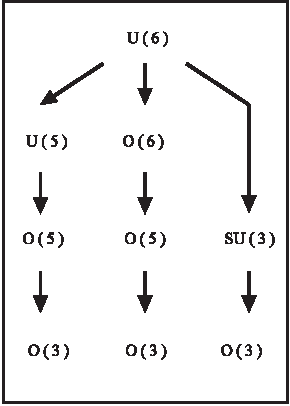
\includegraphics[scale=.65]{figure}
%
% If not, use
%\picplace{5cm}{2cm} % Give the correct figure height and width in cm
%
\caption{Please write your figure caption here}
\label{fig:A1}       % Give a unique label
\end{figure}

% For tables use
%
\begin{table}
\caption{Please write your table caption here}
\label{tab:A1}       % Give a unique label
%
% For LaTeX tables use
%
\begin{tabular}{p{2cm}p{2.4cm}p{2cm}p{4.9cm}}
\hline\noalign{\smallskip}
Classes & Subclass & Length & Action Mechanism  \\
\noalign{\smallskip}\hline\noalign{\smallskip}
Translation & mRNA$^a$  & 22 (19--25) & Translation repression, mRNA cleavage\\
Translation & mRNA cleavage & 21 & mRNA cleavage\\
Translation & mRNA  & 21--22 & mRNA cleavage\\
Translation & mRNA  & 24--26 & Histone and DNA Modification\\
\noalign{\smallskip}\hline\noalign{\smallskip}
\end{tabular}
$^a$ Table foot note (with superscript)
\end{table}
%

% %%%%%%%%%%%%%%%%%%%%%%acronym.tex%%%%%%%%%%%%%%%%%%%%%%%%%%%%%%%%%%%%%%%%%
% sample list of acronyms
%
% Use this file as a template for your own input.
%
%%%%%%%%%%%%%%%%%%%%%%%% Springer %%%%%%%%%%%%%%%%%%%%%%%%%%

\Extrachap{Glossary}



% 
\Extrachap{Solutions}

\section*{Problems of Chapter~\ref{intro}}

\begin{sol}{prob1}
The solution\index{problems}\index{solutions} is revealed here.
\end{sol}


\begin{sol}{prob2}
\textbf{Problem Heading}\\
(a) The solution of first part is revealed here.\\
(b) The solution of second part is revealed here.
\end{sol}


\printindex

%%%%%%%%%%%%%%%%%%%%%%%%%%%%%%%%%%%%%%%%%%%%%%%%%%%%%%%%%%%%%%%%%%%%%%

\end{document}





